% Counting & Probability -- a visual mini-textbook
% Benjamin Michael Haire -- https://theisegoria.github.io/
% Single-file LaTeX source. Compile with:  pdflatex counting-and-probability.tex  (three times)

\documentclass[11pt,a4paper]{article}
% ---- begin preamble.tex ----
% ============================================================
%  Preamble : Counting & Probability mini-textbook
% ============================================================
\usepackage[a4paper,top=2.4cm,bottom=2.4cm,left=2.3cm,right=2.3cm,headsep=14pt,footskip=26pt]{geometry}

\usepackage{amsmath,amssymb,amsthm,mathtools,bm}
\usepackage[T1]{fontenc}
\usepackage{mathpazo}
\usepackage{avant}   % Avant Garde for headings (sans)
\usepackage{microtype}
\usepackage{xcolor}
\usepackage{graphicx}
\usepackage{booktabs,array,tabularx,multirow,colortbl,longtable}
\usepackage{enumitem}
\usepackage[most]{tcolorbox}
\usepackage{tikz}
\usepackage{pgfplots}
\usepackage{fancyhdr}
\usepackage{titlesec}
\usepackage{titletoc}
\usepackage{float}
\usepackage{caption}
\usepackage[hidelinks]{hyperref}
\usepackage{needspace}
\usepackage{ifthen}
\usepackage{multicol}

\pgfplotsset{compat=1.18}
\usetikzlibrary{arrows.meta,positioning,calc,decorations.pathreplacing,
                shapes.geometric,patterns,fit,backgrounds,shadows.blur,math,fadings}

% ------------------------------------------------------------
%  Palette
% ------------------------------------------------------------
\definecolor{ink}      {HTML}{16202E}
\definecolor{indigo}   {HTML}{33527E}
\definecolor{indigoLt} {HTML}{E8EDF6}
\definecolor{teal}     {HTML}{1F7A6B}
\definecolor{tealLt}   {HTML}{E3F2EE}
\definecolor{amber}    {HTML}{B87421}
\definecolor{amberLt}  {HTML}{FBF0DE}
\definecolor{rose}     {HTML}{A8434C}
\definecolor{roseLt}   {HTML}{FAEAEB}
\definecolor{plum}     {HTML}{6B4A7E}
\definecolor{plumLt}   {HTML}{F0EAF5}
\definecolor{slate}    {HTML}{5B6B7F}
\definecolor{paper}    {HTML}{FAF8F4}
\definecolor{rule}     {HTML}{C9CFD9}

\hypersetup{colorlinks=true,linkcolor=indigo,urlcolor=teal,
            pdftitle={Counting and Probability},pdfauthor={}}

\pretocmd{\section}{\needspace{6\baselineskip}}{}{}
\pretocmd{\subsection}{\needspace{4\baselineskip}}{}{}

% ------------------------------------------------------------
%  Headings
% ------------------------------------------------------------
\titleformat{\section}[hang]
  {\sffamily\bfseries\Large\color{ink}}
  {\colorbox{indigo}{\textcolor{white}{\sffamily\bfseries\ \thesection\ }}\;}
  {0.5em}{}[\vspace{2pt}{\color{rule}\titlerule[0.8pt]}]
\titlespacing*{\section}{0pt}{2.2ex plus 1ex minus .2ex}{1.4ex plus .2ex}

\titleformat{\subsection}[hang]
  {\sffamily\bfseries\large\color{indigo}}{\thesubsection}{0.6em}{}
\titlespacing*{\subsection}{0pt}{2.0ex plus 1ex minus .2ex}{0.9ex plus .2ex}

\titleformat{\subsubsection}[runin]
  {\sffamily\bfseries\color{teal}}{}{0pt}{}[\;---\;]
\titlespacing*{\subsubsection}{0pt}{1.4ex}{0.6em}

% Part pages
\titleformat{\part}[display]
  {\sffamily\bfseries\color{indigo}\filcenter}
  {\normalsize\MakeUppercase{\partname~\thepart}\vspace{4pt}}
  {6pt}{\Huge}
\titlespacing*{\part}{0pt}{40pt}{22pt}

% ------------------------------------------------------------
%  Running heads
% ------------------------------------------------------------
\pagestyle{fancy}
\fancyhf{}
\renewcommand{\headrulewidth}{0pt}
\renewcommand{\footrulewidth}{0pt}
\fancyhead[L]{\sffamily\scriptsize\color{slate}\MakeUppercase{Counting \& Probability}}
\fancyhead[R]{\sffamily\scriptsize\color{slate}\nouppercase{\leftmark}}
\fancyfoot[C]{\sffamily\small\color{slate}\thepage}
\renewcommand{\sectionmark}[1]{\markboth{#1}{}}
\fancypagestyle{plain}{\fancyhf{}\fancyfoot[C]{\sffamily\small\color{slate}\thepage}%
  \renewcommand{\headrulewidth}{0pt}}

% ------------------------------------------------------------
%  Boxes
% ------------------------------------------------------------
\newtcolorbox{defbox}[1][]{
  enhanced, breakable, colback=indigoLt, colframe=indigo,
  boxrule=0pt, leftrule=2.6pt, arc=1.5pt, left=8pt,right=8pt,top=6pt,bottom=6pt,
  fonttitle=\sffamily\bfseries\small, coltitle=indigo,
  attach boxed title to top left={yshift=-2.4mm,xshift=6mm},
  boxed title style={colback=indigoLt,boxrule=0pt,arc=0pt,left=3pt,right=3pt},
  title={#1}}

\newtcolorbox{thmbox}[1][]{
  enhanced, breakable, colback=tealLt, colframe=teal,
  boxrule=0pt, leftrule=2.6pt, arc=1.5pt, left=8pt,right=8pt,top=6pt,bottom=6pt,
  fonttitle=\sffamily\bfseries\small, coltitle=teal,
  attach boxed title to top left={yshift=-2.4mm,xshift=6mm},
  boxed title style={colback=tealLt,boxrule=0pt,arc=0pt,left=3pt,right=3pt},
  title={#1}}

\newtcolorbox{exbox}[1][]{
  enhanced, breakable, colback=amberLt, colframe=amber,
  boxrule=0pt, leftrule=2.6pt, arc=1.5pt, left=8pt,right=8pt,top=6pt,bottom=6pt,
  fonttitle=\sffamily\bfseries\small, coltitle=amber,
  attach boxed title to top left={yshift=-2.4mm,xshift=6mm},
  boxed title style={colback=amberLt,boxrule=0pt,arc=0pt,left=3pt,right=3pt},
  title={#1}}

\newtcolorbox{warnbox}[1][Watch out]{
  enhanced, breakable, colback=roseLt, colframe=rose,
  boxrule=0pt, leftrule=2.6pt, arc=1.5pt, left=8pt,right=8pt,top=6pt,bottom=6pt,
  fonttitle=\sffamily\bfseries\small, coltitle=rose,
  attach boxed title to top left={yshift=-2.4mm,xshift=6mm},
  boxed title style={colback=roseLt,boxrule=0pt,arc=0pt,left=3pt,right=3pt},
  title={#1}}

\newtcolorbox{ideabox}[1][The idea]{
  enhanced, breakable, colback=plumLt, colframe=plum,
  boxrule=0pt, leftrule=2.6pt, arc=1.5pt, left=8pt,right=8pt,top=6pt,bottom=6pt,
  fonttitle=\sffamily\bfseries\small, coltitle=plum,
  attach boxed title to top left={yshift=-2.4mm,xshift=6mm},
  boxed title style={colback=plumLt,boxrule=0pt,arc=0pt,left=3pt,right=3pt},
  title={#1}}

% A quiet framed box for summary panels
\newtcolorbox{panel}[1][]{
  enhanced, breakable, colback=paper, colframe=rule,
  boxrule=0.7pt, arc=2pt, left=9pt,right=9pt,top=7pt,bottom=7pt,
  fonttitle=\sffamily\bfseries\small, coltitle=ink,
  attach boxed title to top left={yshift=-2.6mm,xshift=6mm},
  boxed title style={colback=paper,boxrule=0.7pt,colframe=rule,arc=1pt,left=4pt,right=4pt},
  title={#1}}

% ------------------------------------------------------------
%  Macros
% ------------------------------------------------------------
\DeclareMathOperator{\Var}{Var}
\DeclareMathOperator{\Cov}{Cov}
\DeclareMathOperator{\Corr}{Corr}
\DeclareMathOperator{\SD}{SD}
\DeclareMathOperator{\sgn}{sgn}
\DeclareMathOperator{\lcm}{lcm}
\newcommand{\E}{\mathbb{E}}
\newcommand{\Prob}{\mathbb{P}}
\newcommand{\R}{\mathbb{R}}
\newcommand{\N}{\mathbb{N}}
\newcommand{\Z}{\mathbb{Z}}
\newcommand{\one}{\mathbf{1}}
\newcommand{\dd}{\,\mathrm{d}}
\newcommand{\perm}[2]{P(#1,#2)}
\newcommand{\comb}[2]{\binom{#1}{#2}}
\newcommand{\given}{\mathbin{\vert}}
\newcommand{\eqdef}{\vcentcolon=}
\newcommand{\ffact}[2]{#1^{\underline{#2}}}   % falling factorial
\newcommand{\rfact}[2]{#1^{\overline{#2}}}    % rising factorial
\newcommand{\keyw}[1]{\textcolor{indigo}{\textbf{#1}}}
\newcommand{\smallcaps}[1]{\textsc{#1}}

% Nice "answer" tag
\newcommand{\ans}[1]{\;\boxed{\,#1\,}}

% list tuning
\setlist[itemize]{leftmargin=1.35em,topsep=3pt,itemsep=2pt,parsep=0pt}
\setlist[enumerate]{leftmargin=1.6em,topsep=3pt,itemsep=2pt,parsep=0pt}

% caption style
\captionsetup{font=small,labelfont={sf,bf,color=indigo},textfont=it,width=0.9\textwidth}

% spacing
\setlength{\parskip}{4pt}
\setlength{\parindent}{0pt}
\renewcommand{\arraystretch}{1.18}
% ---- end preamble.tex ----
\begin{document}
% ---- begin titlepage.tex ----
% ============================ TITLE PAGE ============================
\begin{titlepage}
\thispagestyle{empty}
\begin{tikzpicture}[remember picture, overlay]
  \fill[paper] (current page.south west) rectangle (current page.north east);

  \begin{scope}[shift={($(current page.north)+(0,-1.6cm)$)}]
% ---- begin pascalfield.tex ----
% auto-generated Pascal disc field
\fill[indigo,opacity=0.13] (0.0,0.0) circle (0.215);
\fill[indigo,opacity=0.13] (-0.35,-0.6) circle (0.215);
\fill[indigo,opacity=0.13] (0.35,-0.6) circle (0.215);
\fill[indigo,opacity=0.13] (-0.7,-1.2) circle (0.215);
\fill[indigo,opacity=0.183] (0.0,-1.2) circle (0.215);
\fill[indigo,opacity=0.13] (0.7,-1.2) circle (0.215);
\fill[indigo,opacity=0.13] (-1.05,-1.8) circle (0.215);
\fill[indigo,opacity=0.214] (-0.35,-1.8) circle (0.215);
\fill[indigo,opacity=0.214] (0.35,-1.8) circle (0.215);
\fill[indigo,opacity=0.13] (1.05,-1.8) circle (0.215);
\fill[indigo,opacity=0.13] (-1.4,-2.4) circle (0.215);
\fill[indigo,opacity=0.235] (-0.7,-2.4) circle (0.215);
\fill[indigo,opacity=0.266] (0.0,-2.4) circle (0.215);
\fill[indigo,opacity=0.235] (0.7,-2.4) circle (0.215);
\fill[indigo,opacity=0.13] (1.4,-2.4) circle (0.215);
\fill[indigo,opacity=0.13] (-1.75,-3.0) circle (0.215);
\fill[indigo,opacity=0.252] (-1.05,-3.0) circle (0.215);
\fill[indigo,opacity=0.305] (-0.35,-3.0) circle (0.215);
\fill[indigo,opacity=0.305] (0.35,-3.0) circle (0.215);
\fill[indigo,opacity=0.252] (1.05,-3.0) circle (0.215);
\fill[indigo,opacity=0.13] (1.75,-3.0) circle (0.215);
\fill[indigo,opacity=0.13] (-2.1,-3.6) circle (0.215);
\fill[indigo,opacity=0.266] (-1.4,-3.6) circle (0.215);
\fill[indigo,opacity=0.336] (-0.7,-3.6) circle (0.215);
\fill[indigo,opacity=0.358] (0.0,-3.6) circle (0.215);
\fill[indigo,opacity=0.336] (0.7,-3.6) circle (0.215);
\fill[indigo,opacity=0.266] (1.4,-3.6) circle (0.215);
\fill[indigo,opacity=0.13] (2.1,-3.6) circle (0.215);
\fill[indigo,opacity=0.13] (-2.45,-4.2) circle (0.215);
\fill[indigo,opacity=0.278] (-1.75,-4.2) circle (0.215);
\fill[indigo,opacity=0.362] (-1.05,-4.2) circle (0.215);
\fill[indigo,opacity=0.401] (-0.35,-4.2) circle (0.215);
\fill[indigo,opacity=0.401] (0.35,-4.2) circle (0.215);
\fill[indigo,opacity=0.362] (1.05,-4.2) circle (0.215);
\fill[indigo,opacity=0.278] (1.75,-4.2) circle (0.215);
\fill[indigo,opacity=0.13] (2.45,-4.2) circle (0.215);
\fill[indigo,opacity=0.13] (-2.8,-4.8) circle (0.215);
\fill[indigo,opacity=0.288] (-2.1,-4.8) circle (0.215);
\fill[indigo,opacity=0.384] (-1.4,-4.8) circle (0.215);
\fill[indigo,opacity=0.436] (-0.7,-4.8) circle (0.215);
\fill[indigo,opacity=0.453] (0.0,-4.8) circle (0.215);
\fill[indigo,opacity=0.436] (0.7,-4.8) circle (0.215);
\fill[indigo,opacity=0.384] (1.4,-4.8) circle (0.215);
\fill[indigo,opacity=0.288] (2.1,-4.8) circle (0.215);
\fill[indigo,opacity=0.13] (2.8,-4.8) circle (0.215);
\fill[indigo,opacity=0.13] (-3.15,-5.4) circle (0.215);
\fill[indigo,opacity=0.297] (-2.45,-5.4) circle (0.215);
\fill[indigo,opacity=0.403] (-1.75,-5.4) circle (0.215);
\fill[indigo,opacity=0.467] (-1.05,-5.4) circle (0.215);
\fill[indigo,opacity=0.498] (-0.35,-5.4) circle (0.215);
\fill[indigo,opacity=0.498] (0.35,-5.4) circle (0.215);
\fill[indigo,opacity=0.467] (1.05,-5.4) circle (0.215);
\fill[indigo,opacity=0.403] (1.75,-5.4) circle (0.215);
\fill[indigo,opacity=0.297] (2.45,-5.4) circle (0.215);
\fill[indigo,opacity=0.13] (3.15,-5.4) circle (0.215);
\fill[indigo,opacity=0.13] (-3.5,-6.0) circle (0.215);
\fill[indigo,opacity=0.305] (-2.8,-6.0) circle (0.215);
\fill[indigo,opacity=0.42] (-2.1,-6.0) circle (0.215);
\fill[indigo,opacity=0.494] (-1.4,-6.0) circle (0.215);
\fill[indigo,opacity=0.537] (-0.7,-6.0) circle (0.215);
\fill[indigo,opacity=0.551] (0.0,-6.0) circle (0.215);
\fill[indigo,opacity=0.537] (0.7,-6.0) circle (0.215);
\fill[indigo,opacity=0.494] (1.4,-6.0) circle (0.215);
\fill[indigo,opacity=0.42] (2.1,-6.0) circle (0.215);
\fill[indigo,opacity=0.305] (2.8,-6.0) circle (0.215);
\fill[indigo,opacity=0.13] (3.5,-6.0) circle (0.215);
\fill[indigo,opacity=0.13] (-3.85,-6.6) circle (0.215);
\fill[indigo,opacity=0.312] (-3.15,-6.6) circle (0.215);
\fill[indigo,opacity=0.435] (-2.45,-6.6) circle (0.215);
\fill[indigo,opacity=0.519] (-1.75,-6.6) circle (0.215);
\fill[indigo,opacity=0.571] (-1.05,-6.6) circle (0.215);
\fill[indigo,opacity=0.597] (-0.35,-6.6) circle (0.215);
\fill[indigo,opacity=0.597] (0.35,-6.6) circle (0.215);
\fill[indigo,opacity=0.571] (1.05,-6.6) circle (0.215);
\fill[indigo,opacity=0.519] (1.75,-6.6) circle (0.215);
\fill[indigo,opacity=0.435] (2.45,-6.6) circle (0.215);
\fill[indigo,opacity=0.312] (3.15,-6.6) circle (0.215);
\fill[indigo,opacity=0.13] (3.85,-6.6) circle (0.215);
\fill[indigo,opacity=0.13] (-4.2,-7.2) circle (0.215);
\fill[indigo,opacity=0.319] (-3.5,-7.2) circle (0.215);
\fill[indigo,opacity=0.449] (-2.8,-7.2) circle (0.215);
\fill[indigo,opacity=0.54] (-2.1,-7.2) circle (0.215);
\fill[indigo,opacity=0.602] (-1.4,-7.2) circle (0.215);
\fill[indigo,opacity=0.638] (-0.7,-7.2) circle (0.215);
\fill[indigo,opacity=0.65] (0.0,-7.2) circle (0.215);
\fill[indigo,opacity=0.638] (0.7,-7.2) circle (0.215);
\fill[indigo,opacity=0.602] (1.4,-7.2) circle (0.215);
\fill[indigo,opacity=0.54] (2.1,-7.2) circle (0.215);
\fill[indigo,opacity=0.449] (2.8,-7.2) circle (0.215);
\fill[indigo,opacity=0.319] (3.5,-7.2) circle (0.215);
\fill[indigo,opacity=0.13] (4.2,-7.2) circle (0.215);
\fill[indigo,opacity=0.13] (-4.55,-7.8) circle (0.215);
\fill[indigo,opacity=0.325] (-3.85,-7.8) circle (0.215);
\fill[indigo,opacity=0.461] (-3.15,-7.8) circle (0.215);
\fill[indigo,opacity=0.56] (-2.45,-7.8) circle (0.215);
\fill[indigo,opacity=0.63] (-1.75,-7.8) circle (0.215);
\fill[indigo,opacity=0.675] (-1.05,-7.8) circle (0.215);
\fill[indigo,opacity=0.697] (-0.35,-7.8) circle (0.215);
\fill[indigo,opacity=0.697] (0.35,-7.8) circle (0.215);
\fill[indigo,opacity=0.675] (1.05,-7.8) circle (0.215);
\fill[indigo,opacity=0.63] (1.75,-7.8) circle (0.215);
\fill[indigo,opacity=0.56] (2.45,-7.8) circle (0.215);
\fill[indigo,opacity=0.461] (3.15,-7.8) circle (0.215);
\fill[indigo,opacity=0.325] (3.85,-7.8) circle (0.215);
\fill[indigo,opacity=0.13] (4.55,-7.8) circle (0.215);
\fill[indigo,opacity=0.13] (-4.9,-8.4) circle (0.215);
\fill[indigo,opacity=0.331] (-4.2,-8.4) circle (0.215);
\fill[indigo,opacity=0.473] (-3.5,-8.4) circle (0.215);
\fill[indigo,opacity=0.579] (-2.8,-8.4) circle (0.215);
\fill[indigo,opacity=0.656] (-2.1,-8.4) circle (0.215);
\fill[indigo,opacity=0.708] (-1.4,-8.4) circle (0.215);
\fill[indigo,opacity=0.739] (-0.7,-8.4) circle (0.215);
\fill[indigo,opacity=0.749] (0.0,-8.4) circle (0.215);
\fill[indigo,opacity=0.739] (0.7,-8.4) circle (0.215);
\fill[indigo,opacity=0.708] (1.4,-8.4) circle (0.215);
\fill[indigo,opacity=0.656] (2.1,-8.4) circle (0.215);
\fill[indigo,opacity=0.579] (2.8,-8.4) circle (0.215);
\fill[indigo,opacity=0.473] (3.5,-8.4) circle (0.215);
\fill[indigo,opacity=0.331] (4.2,-8.4) circle (0.215);
\fill[indigo,opacity=0.13] (4.9,-8.4) circle (0.215);
\fill[indigo,opacity=0.13] (-5.25,-9.0) circle (0.215);
\fill[indigo,opacity=0.336] (-4.55,-9.0) circle (0.215);
\fill[indigo,opacity=0.484] (-3.85,-9.0) circle (0.215);
\fill[indigo,opacity=0.596] (-3.15,-9.0) circle (0.215);
\fill[indigo,opacity=0.679] (-2.45,-9.0) circle (0.215);
\fill[indigo,opacity=0.739] (-1.75,-9.0) circle (0.215);
\fill[indigo,opacity=0.778] (-1.05,-9.0) circle (0.215);
\fill[indigo,opacity=0.797] (-0.35,-9.0) circle (0.215);
\fill[indigo,opacity=0.797] (0.35,-9.0) circle (0.215);
\fill[indigo,opacity=0.778] (1.05,-9.0) circle (0.215);
\fill[indigo,opacity=0.739] (1.75,-9.0) circle (0.215);
\fill[indigo,opacity=0.679] (2.45,-9.0) circle (0.215);
\fill[indigo,opacity=0.596] (3.15,-9.0) circle (0.215);
\fill[indigo,opacity=0.484] (3.85,-9.0) circle (0.215);
\fill[indigo,opacity=0.336] (4.55,-9.0) circle (0.215);
\fill[indigo,opacity=0.13] (5.25,-9.0) circle (0.215);
\fill[indigo,opacity=0.13] (-5.6,-9.6) circle (0.215);
\fill[indigo,opacity=0.341] (-4.9,-9.6) circle (0.215);
\fill[indigo,opacity=0.494] (-4.2,-9.6) circle (0.215);
\fill[indigo,opacity=0.611] (-3.5,-9.6) circle (0.215);
\fill[indigo,opacity=0.701] (-2.8,-9.6) circle (0.215);
\fill[indigo,opacity=0.768] (-2.1,-9.6) circle (0.215);
\fill[indigo,opacity=0.814] (-1.4,-9.6) circle (0.215);
\fill[indigo,opacity=0.841] (-0.7,-9.6) circle (0.215);
\fill[indigo,opacity=0.85] (0.0,-9.6) circle (0.215);
\fill[indigo,opacity=0.841] (0.7,-9.6) circle (0.215);
\fill[indigo,opacity=0.814] (1.4,-9.6) circle (0.215);
\fill[indigo,opacity=0.768] (2.1,-9.6) circle (0.215);
\fill[indigo,opacity=0.701] (2.8,-9.6) circle (0.215);
\fill[indigo,opacity=0.611] (3.5,-9.6) circle (0.215);
\fill[indigo,opacity=0.494] (4.2,-9.6) circle (0.215);
\fill[indigo,opacity=0.341] (4.9,-9.6) circle (0.215);
\fill[indigo,opacity=0.13] (5.6,-9.6) circle (0.215);
% ---- end pascalfield.tex ----
  \end{scope}

  % smooth fade of the triangle into the page
  \fill[paper, path fading=north]
    ($(current page.north west)+(0,-8.0cm)$) rectangle ($(current page.north east)+(0,-12.2cm)$);
  \fill[paper]
    ($(current page.north west)+(0,-12.2cm)$) rectangle (current page.south east);
\end{tikzpicture}

\vspace*{10.4cm}

\begin{flushleft}
{\color{amber}\rule{3.2cm}{2pt}}\\[10pt]
{\sffamily\fontsize{12}{15}\selectfont\color{amber}\bfseries A VISUAL MINI-TEXTBOOK}\\[12pt]
{\sffamily\bfseries\fontsize{46}{50}\selectfont\color{ink} Counting}\\[2pt]
{\sffamily\bfseries\fontsize{46}{50}\selectfont\color{ink} \&\ Probability}\\[18pt]
{\sffamily\fontsize{13}{19}\selectfont\color{slate}
 From the product rule to Poisson: permutations, combinations,\\
 the binomial theorem, and the probability they generate.}
\end{flushleft}

\vspace{1.1cm}
{\color{rule}\rule{\textwidth}{0.7pt}}
\vspace{0.5cm}

{\sffamily\small\color{ink}
\begin{tabular}{@{}p{0.29\textwidth}p{0.29\textwidth}p{0.29\textwidth}@{}}
  \textcolor{indigo}{\bfseries I.}~~Counting &
  \textcolor{indigo}{\bfseries II.}~~Probability &
  \textcolor{indigo}{\bfseries III.}~~Reference \\[4pt]
  {\footnotesize\color{slate}Rules of counting, $\perm{n}{k}$ and $\comb{n}{k}$,
    Pascal identities, the binomial and multinomial theorems, stars and bars,
    inclusion--exclusion, bijections.} &
  {\footnotesize\color{slate}Axioms, conditional probability and Bayes,
    expectation by indicators, variance, the named discrete
    distributions, classic problems.} &
  {\footnotesize\color{slate}A formula spread, a distribution table,
    a ``which formula do I use?'' decision guide, and problems with
    full solutions.}
\end{tabular}}

\par\vspace*{\fill}
{\sffamily\footnotesize\color{slate} Prepared for Ben \quad\textbullet\quad \today}
\end{titlepage}
% ---- end titlepage.tex ----
\clearpage
\pagenumbering{roman}
% ---- begin toc.tex ----
{\sffamily\bfseries\LARGE\color{ink} Contents}
\vspace{4pt}\\
{\color{rule}\rule{\textwidth}{0.8pt}}
\vspace{-6pt}

\setcounter{tocdepth}{2}
\titlecontents{part}[0pt]
  {\vspace{10pt}\sffamily\bfseries\color{indigo}}
  {}{}{}
\titlecontents{section}[1.6em]
  {\vspace{3pt}\sffamily}
  {\contentslabel{1.6em}}{}
  {\titlerule*[0.7pc]{\color{rule}.}\contentspage}
\titlecontents{subsection}[3.6em]
  {\sffamily\small\color{slate}}
  {\contentslabel{2.2em}}{}
  {\titlerule*[0.7pc]{\color{rule}.}\contentspage}
\makeatletter\@starttoc{toc}\makeatother
% ---- end toc.tex ----
\clearpage
\pagenumbering{arabic}
% ---- begin ch00-orientation.tex ----
\section*{How to read this}
\addcontentsline{toc}{section}{How to read this}
\markboth{How to read this}{}

Everything in the first half of this book is one idea wearing different hats:
\emph{if you can describe an object uniquely by a sequence of independent choices,
you can count the objects by multiplying the number of choices.} Permutations,
combinations, $\comb{n}{k}$, the binomial theorem, stars and bars: all of them are
that sentence, plus a correction for overcounting.

Everything in the second half is one further idea: \emph{probability on a finite
set where every outcome is equally likely is nothing but counting, divided.}
Once outcomes stop being equally likely you need the axioms, and once you want
averages you need expectation, but the counting never goes away.

\begin{ideabox}[The two-line summary of the whole book]
\textbf{Counting.} Build the object by a sequence of choices; multiply; then divide by
the number of times you built the same object twice.

\textbf{Probability.} $\Prob(A) = \dfrac{\lvert A\rvert}{\lvert S\rvert}$ when outcomes are
equally likely; otherwise use the axioms; and when you want an average, use
$\E\!\left[\sum_i X_i\right] = \sum_i \E[X_i]$, which never asks whether the $X_i$
are independent.
\end{ideabox}

\subsection*{Conventions used throughout}

\begin{panel}[Notation]
\begin{tabularx}{\textwidth}{@{}lX@{}}
\toprule
$n!$ & $n\cdot(n-1)\cdots 2\cdot 1$, with $0! = 1$. \\
$\perm{n}{k}$, $\ffact{n}{k}$ & the number of ordered $k$-selections from $n$ distinct objects;
   also written $^nP_k$ or $n^{\underline{k}}$ (the \emph{falling factorial}). \\
$\comb{n}{k}$ & the number of unordered $k$-subsets of an $n$-set; also written
   $^nC_k$, $C(n,k)$, or ``$n$ choose $k$''. \\
$\rfact{n}{k}$ & the \emph{rising factorial} $n(n+1)\cdots(n+k-1)$. \\
$[n]$ & the set $\{1,2,\dots,n\}$. \\
$\lvert A\rvert$ & the number of elements of the finite set $A$. \\
$S$ & the sample space; $A, B, C$ denote events (subsets of $S$). \\
$\one_A$ & the indicator random variable of the event $A$: $1$ if $A$ happens, $0$ if not. \\
$X \sim \mathcal{D}$ & the random variable $X$ has distribution $\mathcal{D}$. \\
\bottomrule
\end{tabularx}
\end{panel}

\subsection*{The colour code}

\begin{itemize}
  \item \textcolor{indigo}{\textbf{Blue boxes}} are definitions: what a symbol means.
  \item \textcolor{teal}{\textbf{Green boxes}} are theorems and identities: what is true.
  \item \textcolor{amber}{\textbf{Amber boxes}} are worked examples.
  \item \textcolor{plum}{\textbf{Purple boxes}} are the idea behind the algebra, in words.
  \item \textcolor{rose}{\textbf{Red boxes}} are the mistakes that actually get made.
\end{itemize}

If you read nothing else, read the purple boxes and the reference spread at the end.
% ---- end ch00-orientation.tex ----
\clearpage
\part{Counting}
% ---- begin ch01-foundations.tex ----
\section{The two rules everything is built from}

There are exactly two counting rules. Every formula later in this book is a
consequence of applying them carefully and then correcting for overcounting.

\begin{defbox}[The sum rule]
If a set $A$ can be split into pieces $A_1, A_2, \dots, A_m$ that are
\emph{pairwise disjoint} (no object lies in two pieces) and together make up all
of $A$, then
\[
  \lvert A\rvert \;=\; \lvert A_1\rvert + \lvert A_2\rvert + \dots + \lvert A_m\rvert .
\]
In words: \keyw{case-split}, then add. The word \emph{or} usually signals a sum.
\end{defbox}

\begin{defbox}[The product rule]
If an object is built by making a sequence of $k$ choices, where the $i$th choice
can be made in $n_i$ ways \emph{no matter how the earlier choices went}, then the
number of objects is
\[
  n_1 \, n_2 \cdots n_k .
\]
In words: \keyw{choose in stages}, then multiply. The word \emph{and} usually
signals a product.
\end{defbox}

The clause ``no matter how the earlier choices went'' is the whole game. The
number of options at stage $i$ may \emph{depend} on the earlier choices; what it
may not do is \emph{change in count}. Arranging three of five books on a shelf
gives $5 \times 4 \times 3$: which three books remain available depends entirely
on what you picked first, but \emph{how many} remain does not.

\begin{figure}[H]
\centering
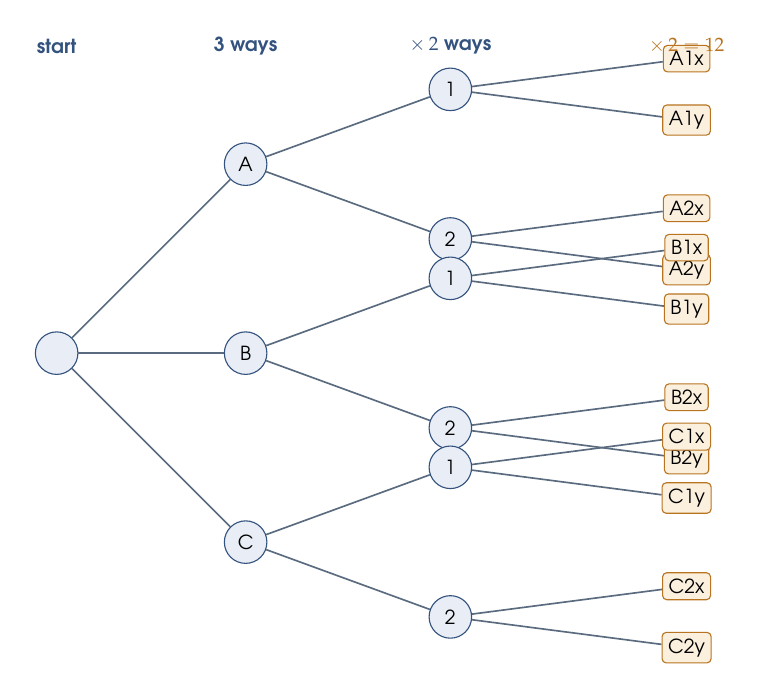
\begin{tikzpicture}[
   lvl/.style={circle, draw=indigo, fill=indigoLt, inner sep=0pt, minimum size=5.4mm,
               font=\scriptsize\sffamily},
   leaf/.style={rectangle, draw=amber, fill=amberLt, rounded corners=1.5pt,
                inner sep=2.2pt, font=\scriptsize\sffamily},
   edge/.style={draw=slate, line width=0.6pt}
]
\node[lvl] (r) at (0,0) {};
\foreach \i/\lab in {1/A,2/B,3/C}{
  \pgfmathsetmacro{\y}{2.4-(\i-1)*2.4}
  \node[lvl] (a\i) at (2.4,\y) {\lab};
  \draw[edge] (r) -- (a\i);
}
\foreach \i in {1,2,3}{
  \foreach \j in {1,2}{
    \pgfmathsetmacro{\yy}{2.4-(\i-1)*2.4 + (1.5-\j)*1.9}
    \node[lvl] (b\i\j) at (5.0,\yy) {\j};
    \draw[edge] (a\i) -- (b\i\j);
  }
}
\foreach \i/\lab in {1/A,2/B,3/C}{
  \foreach \j in {1,2}{
    \foreach \k/\s in {1/x,2/y}{
      \pgfmathsetmacro{\yyy}{2.4-(\i-1)*2.4 + (1.5-\j)*1.9 + (1.5-\k)*0.78}
      \node[leaf] (c\i\j\k) at (8.0,\yyy) {\lab\j\s};
      \draw[edge] (b\i\j) -- (c\i\j\k);
    }
  }
}
\node[font=\scriptsize\sffamily\bfseries, color=indigo] at (0,3.9) {start};
\node[font=\scriptsize\sffamily\bfseries, color=indigo] at (2.4,3.9) {3 ways};
\node[font=\scriptsize\sffamily\bfseries, color=indigo] at (5.0,3.9) {$\times\,2$ ways};
\node[font=\scriptsize\sffamily\bfseries, color=amber]  at (8.0,3.9) {$\times\,2 = 12$};
\end{tikzpicture}
\caption{The product rule is a tree. Each leaf is one object; the number of leaves is
the product of the branching factors, provided every node at a given depth has the
same number of children.}
\end{figure}

\subsection{Three corollaries you will use constantly}

\begin{thmbox}[Immediate consequences]
Let $A$ and $B$ be finite sets, $\lvert A\rvert=m$, $\lvert B\rvert=n$.
\begin{enumerate}[label=\textbf{\arabic*.}]
  \item \keyw{Strings.} The number of functions $A \to B$, equivalently the number of
        length-$m$ strings over an alphabet of size $n$, is $n^m$.
        (Product rule: $n$ choices for each of the $m$ inputs.)
  \item \keyw{Subsets.} The number of subsets of $A$ is $2^m$.
        (Each element is in or out: a function $A \to \{\text{in},\text{out}\}$.)
  \item \keyw{Complement.} If $A \subseteq S$, then
        $\lvert A\rvert = \lvert S\rvert - \lvert S \setminus A\rvert$.
        Counting the objects you do \emph{not} want is often far easier.
\end{enumerate}
\end{thmbox}

\begin{exbox}[At least one]
How many strings of length $8$ over $\{a,b,c\}$ contain at least one $a$?

Counting directly means splitting on how many $a$'s appear: eight cases. Counting the
complement means counting strings with \emph{no} $a$, which is just strings over
$\{b,c\}$:
\[
  3^8 - 2^8 \;=\; 6561 - 256 \ans{6305}.
\]
\keyw{Rule of thumb.} ``At least one'' almost always wants the complement.
\end{exbox}

\subsection{The bijection principle}

\begin{defbox}[Bijection principle]
If there is a one-to-one correspondence between the elements of $A$ and the elements
of $B$, then $\lvert A\rvert = \lvert B\rvert$.
\end{defbox}

This sounds like a triviality and is in fact the single most powerful technique in
combinatorics. You do not count the hard set; you find an easy set it is secretly the
same as. Section~\ref{sec:bijections} is devoted to it, but here is the flavour:
the number of subsets of $[n]$ equals the number of binary strings of length $n$,
because ``is element $i$ in the subset?'' is exactly ``is bit $i$ a one?''. That
observation converts a set problem into a string problem, and the string problem is
just the product rule.

\begin{warnbox}[The overcounting trap]
The product rule counts \emph{procedures}, not objects. If two different sequences of
choices produce the same object, the product rule counts that object twice. Almost
every combinatorics error is this error. The fix is always the same: if every object
arises from exactly $d$ procedures, divide by $d$. That division is where $\comb{n}{k}$
comes from.
\end{warnbox}
% ---- end ch01-foundations.tex ----
% ---- begin ch02-permutations.tex ----
\section{Permutations: when order matters}

\begin{defbox}[Permutation, and the $k$-permutation $\perm{n}{k}$]
A \keyw{permutation} of a set is an ordering of all its elements. A
\keyw{$k$-permutation} of an $n$-set is an ordered selection of $k$ of its elements,
without repetition. Their counts are
\[
  n! \;=\; n(n-1)\cdots 2\cdot 1,
  \qquad
  \perm{n}{k} \;=\; \frac{n!}{(n-k)!} \;=\; \underbrace{n(n-1)\cdots(n-k+1)}_{k\ \text{factors}}
  \;=\; \ffact{n}{k}.
\]
Conventions: $0! = 1$, $\perm{n}{0}=1$, $\perm{n}{n}=n!$, and $\perm{n}{k}=0$ if $k>n$.
\end{defbox}

The second form of $\perm{n}{k}$ is the one to memorise, because it is the one the
product rule actually produces: $n$ choices for the first slot, $n-1$ for the second,
and so on down to $n-k+1$ for the $k$th. The factorial-quotient form is a
\emph{simplification} of that product, not its origin. Writing $\perm{9}{3}$ as
$9\cdot 8\cdot 7 = 504$ is faster and safer than writing $9!/6!$.

\begin{figure}[H]
\centering
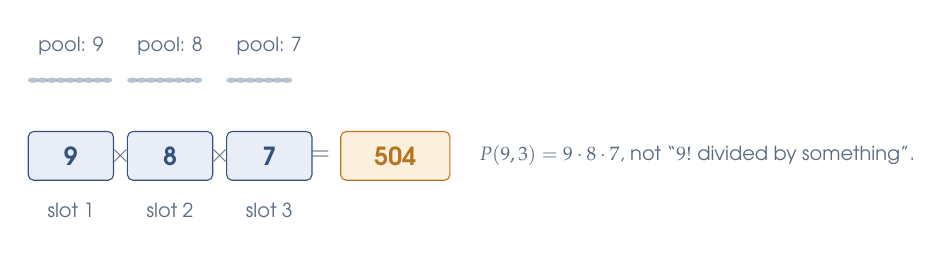
\begin{tikzpicture}[x=1.26cm, y=0.62cm]
  \foreach \i/\n in {0/9,1/8,2/7}{
     \draw[fill=indigoLt, draw=indigo, rounded corners=2pt] (\i,0) rectangle (\i+0.86,1.0);
     \node[font=\small\sffamily\bfseries, color=indigo] at (\i+0.43,0.5) {\n};
     \node[font=\scriptsize\sffamily, color=slate] at (\i+0.43,-0.62) {slot \the\numexpr\i+1\relax};
  }
  \foreach \i in {0,1}{ \node[font=\small, color=slate] at (\i+0.93,0.5) {$\times$}; }
  \node[font=\small, color=slate] at (2.94,0.5) {$=$};
  \draw[fill=amberLt, draw=amber, rounded corners=2pt] (3.15,0) rectangle (4.25,1.0);
  \node[font=\small\sffamily\bfseries, color=amber] at (3.70,0.5) {504};
  \node[font=\scriptsize\sffamily, color=slate, anchor=west] at (4.45,0.5)
       {$\perm{9}{3} = 9\cdot 8\cdot 7$, not ``$9!$ divided by something''.};
  % pool shrinking
  \foreach \i/\m in {0/9,1/8,2/7}{
    \foreach \j in {1,...,\m}{
      \pgfmathsetmacro{\xx}{\i+0.05+(\j-1)*0.093}
      \fill[indigo, opacity=0.35] (\xx,2.05) circle (0.055);
    }
    \node[font=\scriptsize\sffamily, color=slate] at (\i+0.43,2.75) {pool: \m};
  }
\end{tikzpicture}
\caption{A $k$-permutation is the product rule run on a shrinking pool.}
\end{figure}

\subsection{The four flavours of arrangement}

\begin{thmbox}[Arranging things in a row]
\begin{tabularx}{\textwidth}{@{}lXl@{}}
\toprule
\textbf{Situation} & \textbf{Description} & \textbf{Count} \\
\midrule
All $n$ distinct & order all of them & $n!$ \\
$k$ of $n$ distinct & order a selection & $\dfrac{n!}{(n-k)!} = \perm{n}{k}$ \\
$k$ from $n$, repeats allowed & each slot independently & $n^k$ \\
$n$ objects, repeated types & $n_1$ of type $1$, \dots, $n_r$ of type $r$
   & $\dfrac{n!}{n_1!\,n_2!\cdots n_r!}$ \\
\bottomrule
\end{tabularx}
\end{thmbox}

The last line is the \keyw{multinomial coefficient}, written
$\displaystyle\binom{n}{n_1,\,n_2,\,\dots,\,n_r}$. Its derivation is the overcounting
correction in its purest form: pretend the identical objects are distinguishable
(giving $n!$ arrangements), then notice that permuting the $n_1$ copies of type $1$
among themselves changes nothing, and likewise for every other type. Each genuine
arrangement was therefore counted $n_1!\,n_2!\cdots n_r!$ times.

\begin{exbox}[\textsc{mississippi}]
The word \textsc{mississippi} has $11$ letters: one \textsc{m}, four \textsc{i},
four \textsc{s}, two \textsc{p}. The number of distinguishable arrangements is
\[
  \frac{11!}{1!\;4!\;4!\;2!}
  \;=\; \frac{39\,916\,800}{1\cdot 24\cdot 24\cdot 2}
  \ans{34\,650}.
\]
\end{exbox}

\subsection{Circular arrangements}

\begin{thmbox}[Round a table]
The number of ways to seat $n$ distinct people around a circular table, where only
the \emph{relative} order matters, is $(n-1)!$. If the arrangement can also be
flipped over (a necklace, or a table you may view from either side), the count is
$\dfrac{(n-1)!}{2}$ for $n \geq 3$.
\end{thmbox}

Why $(n-1)!$: each circular arrangement corresponds to $n$ linear arrangements, one
for each choice of who is written down first, so $n!/n = (n-1)!$. Equivalently, fix
one person as a reference point and arrange the remaining $n-1$ people relative to
them. The second view is usually the faster one in practice, and it generalises: to
handle a restriction, fix the restricted object first.

\begin{figure}[H]
\centering
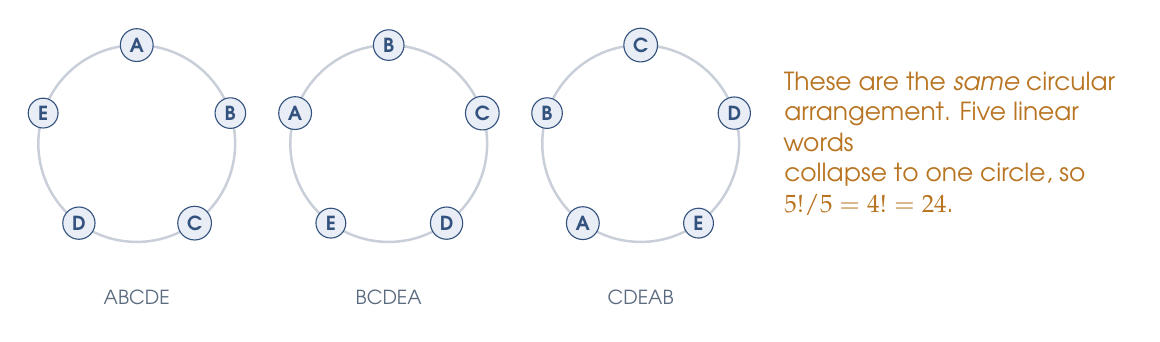
\begin{tikzpicture}
 \begin{scope}
  \draw[rule, line width=0.9pt] (0,0) circle (1.25);
  \foreach \i/\lab in {0/A,1/B,2/C,3/D,4/E}{
    \pgfmathsetmacro{\ang}{90-72*\i}
    \node[circle, fill=indigoLt, draw=indigo, inner sep=1.6pt,
          font=\scriptsize\sffamily\bfseries, text=indigo] at (\ang:1.25) {\lab};
  }
  \node[font=\scriptsize\sffamily, color=slate] at (0,-1.95) {ABCDE};
 \end{scope}
 \begin{scope}[xshift=3.2cm]
  \draw[rule, line width=0.9pt] (0,0) circle (1.25);
  \foreach \i/\lab in {0/B,1/C,2/D,3/E,4/A}{
    \pgfmathsetmacro{\ang}{90-72*\i}
    \node[circle, fill=indigoLt, draw=indigo, inner sep=1.6pt,
          font=\scriptsize\sffamily\bfseries, text=indigo] at (\ang:1.25) {\lab};
  }
  \node[font=\scriptsize\sffamily, color=slate] at (0,-1.95) {BCDEA};
 \end{scope}
 \begin{scope}[xshift=6.4cm]
  \draw[rule, line width=0.9pt] (0,0) circle (1.25);
  \foreach \i/\lab in {0/C,1/D,2/E,3/A,4/B}{
    \pgfmathsetmacro{\ang}{90-72*\i}
    \node[circle, fill=indigoLt, draw=indigo, inner sep=1.6pt,
          font=\scriptsize\sffamily\bfseries, text=indigo] at (\ang:1.25) {\lab};
  }
  \node[font=\scriptsize\sffamily, color=slate] at (0,-1.95) {CDEAB};
 \end{scope}
 \node[font=\small\sffamily, color=amber, anchor=west] at (8.1,0)
   {\begin{minipage}{4.3cm}\raggedright
     These are the \emph{same} circular\\ arrangement. Five linear words\\
     collapse to one circle, so\\ $5!/5 = 4! = 24$.
    \end{minipage}};
\end{tikzpicture}
\caption{Rotations of a circular seating are indistinguishable, so divide by $n$.}
\end{figure}

\subsection{Two standard restriction techniques}

\begin{ideabox}[Glue and gap]
\textbf{Glue (objects must be together).} Treat the block that must stay together as a
single super-object, arrange everything, then multiply by the internal arrangements of
the block. Arranging $7$ people with a specific $3$ insisting on adjacency:
$5!\times 3! = 720$.

\medskip
\textbf{Gap (objects must be apart).} Arrange the unrestricted objects first, then slot
the restricted ones into the gaps between them, at most one per gap. Arranging $5$ boys
and $3$ girls so that no two girls are adjacent: place the boys ($5!$ ways), creating
$6$ gaps, then choose $3$ gaps and order the girls into them
($\perm{6}{3} = 120$). Total $5!\times 120 = 14\,400$.
\end{ideabox}

\begin{warnbox}[$\perm{n}{k}$ versus $n^k$]
$\perm{n}{k}$ is \emph{without} replacement; $n^k$ is \emph{with} replacement. A
four-digit PIN is $10^4$, because digits may repeat. A four-digit PIN with distinct
digits is $\perm{10}{4} = 5040$. Read the problem for the word ``repeat'', ``distinct'',
``replaced'', or ``different'' before writing anything down.
\end{warnbox}
% ---- end ch02-permutations.tex ----
% ---- begin ch03-combinations.tex ----
\section{Combinations: when order does not matter}

\begin{defbox}[The binomial coefficient]
For integers $0 \le k \le n$, the number of $k$-element subsets of an $n$-element set is
\[
  \comb{n}{k} \;=\; \frac{\perm{n}{k}}{k!} \;=\; \frac{n!}{k!\,(n-k)!}
             \;=\; \frac{n(n-1)\cdots(n-k+1)}{k!}.
\]
Set $\comb{n}{k}=0$ when $k<0$ or $k>n$. Read it as ``$n$ choose $k$''.
\end{defbox}

\begin{ideabox}[Why you divide by $k!$]
Count ordered selections: $\perm{n}{k}$. Now ask how many times each \emph{unordered}
$k$-set got counted. Once for every ordering of its $k$ elements, which is $k!$ times,
the same number for every set. So dividing by $k!$ is exact, not an approximation:
\[
  \underbrace{\perm{n}{k}}_{\text{ordered}} \;=\; \underbrace{\comb{n}{k}}_{\text{unordered}} \times \; k! .
\]
Order matters $\Rightarrow$ $\perm{n}{k}$. Order does not $\Rightarrow$ $\comb{n}{k}$.
That is the entire distinction.
\end{ideabox}

\begin{exbox}[Compute it the short way]
$\displaystyle \comb{10}{3} = \frac{10\cdot 9\cdot 8}{3\cdot 2\cdot 1} = \frac{720}{6} = 120$.

$\displaystyle \comb{52}{5} = \frac{52\cdot 51\cdot 50\cdot 49\cdot 48}{120} = 2\,598\,960$
(the number of five-card poker hands).

Never expand the factorials. Cancel as you go: $\comb{100}{2} = \frac{100\cdot 99}{2}=4950$.
\end{exbox}

\subsection{Pascal's triangle}

\begin{figure}[H]
\centering
% ---- begin fig-pascal.tex ----
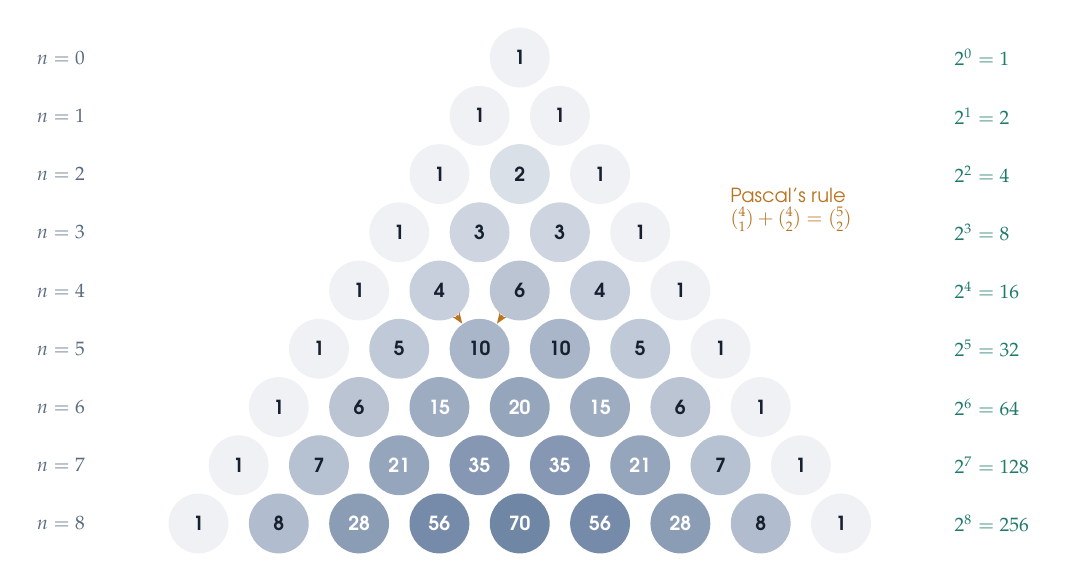
\begin{tikzpicture}[x=1.0cm,y=0.86cm]
\node[circle,fill=indigo!8,inner sep=0pt,minimum size=7.6mm,font=\scriptsize\sffamily\bfseries,text=ink] (n0-0) at (0.0,0.0) {1};
\node[circle,fill=indigo!8,inner sep=0pt,minimum size=7.6mm,font=\scriptsize\sffamily\bfseries,text=ink] (n1-0) at (-0.51,-0.86) {1};
\node[circle,fill=indigo!8,inner sep=0pt,minimum size=7.6mm,font=\scriptsize\sffamily\bfseries,text=ink] (n1-1) at (0.51,-0.86) {1};
\node[circle,fill=indigo!8,inner sep=0pt,minimum size=7.6mm,font=\scriptsize\sffamily\bfseries,text=ink] (n2-0) at (-1.02,-1.72) {1};
\node[circle,fill=indigo!18,inner sep=0pt,minimum size=7.6mm,font=\scriptsize\sffamily\bfseries,text=ink] (n2-1) at (0.0,-1.72) {2};
\node[circle,fill=indigo!8,inner sep=0pt,minimum size=7.6mm,font=\scriptsize\sffamily\bfseries,text=ink] (n2-2) at (1.02,-1.72) {1};
\node[circle,fill=indigo!8,inner sep=0pt,minimum size=7.6mm,font=\scriptsize\sffamily\bfseries,text=ink] (n3-0) at (-1.53,-2.58) {1};
\node[circle,fill=indigo!24,inner sep=0pt,minimum size=7.6mm,font=\scriptsize\sffamily\bfseries,text=ink] (n3-1) at (-0.51,-2.58) {3};
\node[circle,fill=indigo!24,inner sep=0pt,minimum size=7.6mm,font=\scriptsize\sffamily\bfseries,text=ink] (n3-2) at (0.51,-2.58) {3};
\node[circle,fill=indigo!8,inner sep=0pt,minimum size=7.6mm,font=\scriptsize\sffamily\bfseries,text=ink] (n3-3) at (1.53,-2.58) {1};
\node[circle,fill=indigo!8,inner sep=0pt,minimum size=7.6mm,font=\scriptsize\sffamily\bfseries,text=ink] (n4-0) at (-2.04,-3.44) {1};
\node[circle,fill=indigo!28,inner sep=0pt,minimum size=7.6mm,font=\scriptsize\sffamily\bfseries,text=ink] (n4-1) at (-1.02,-3.44) {4};
\node[circle,fill=indigo!34,inner sep=0pt,minimum size=7.6mm,font=\scriptsize\sffamily\bfseries,text=ink] (n4-2) at (0.0,-3.44) {6};
\node[circle,fill=indigo!28,inner sep=0pt,minimum size=7.6mm,font=\scriptsize\sffamily\bfseries,text=ink] (n4-3) at (1.02,-3.44) {4};
\node[circle,fill=indigo!8,inner sep=0pt,minimum size=7.6mm,font=\scriptsize\sffamily\bfseries,text=ink] (n4-4) at (2.04,-3.44) {1};
\node[circle,fill=indigo!8,inner sep=0pt,minimum size=7.6mm,font=\scriptsize\sffamily\bfseries,text=ink] (n5-0) at (-2.55,-4.3) {1};
\node[circle,fill=indigo!31,inner sep=0pt,minimum size=7.6mm,font=\scriptsize\sffamily\bfseries,text=ink] (n5-1) at (-1.53,-4.3) {5};
\node[circle,fill=indigo!42,inner sep=0pt,minimum size=7.6mm,font=\scriptsize\sffamily\bfseries,text=ink] (n5-2) at (-0.51,-4.3) {10};
\node[circle,fill=indigo!42,inner sep=0pt,minimum size=7.6mm,font=\scriptsize\sffamily\bfseries,text=ink] (n5-3) at (0.51,-4.3) {10};
\node[circle,fill=indigo!31,inner sep=0pt,minimum size=7.6mm,font=\scriptsize\sffamily\bfseries,text=ink] (n5-4) at (1.53,-4.3) {5};
\node[circle,fill=indigo!8,inner sep=0pt,minimum size=7.6mm,font=\scriptsize\sffamily\bfseries,text=ink] (n5-5) at (2.55,-4.3) {1};
\node[circle,fill=indigo!8,inner sep=0pt,minimum size=7.6mm,font=\scriptsize\sffamily\bfseries,text=ink] (n6-0) at (-3.06,-5.16) {1};
\node[circle,fill=indigo!34,inner sep=0pt,minimum size=7.6mm,font=\scriptsize\sffamily\bfseries,text=ink] (n6-1) at (-2.04,-5.16) {6};
\node[circle,fill=indigo!48,inner sep=0pt,minimum size=7.6mm,font=\scriptsize\sffamily\bfseries,text=white] (n6-2) at (-1.02,-5.16) {15};
\node[circle,fill=indigo!52,inner sep=0pt,minimum size=7.6mm,font=\scriptsize\sffamily\bfseries,text=white] (n6-3) at (0.0,-5.16) {20};
\node[circle,fill=indigo!48,inner sep=0pt,minimum size=7.6mm,font=\scriptsize\sffamily\bfseries,text=white] (n6-4) at (1.02,-5.16) {15};
\node[circle,fill=indigo!34,inner sep=0pt,minimum size=7.6mm,font=\scriptsize\sffamily\bfseries,text=ink] (n6-5) at (2.04,-5.16) {6};
\node[circle,fill=indigo!8,inner sep=0pt,minimum size=7.6mm,font=\scriptsize\sffamily\bfseries,text=ink] (n6-6) at (3.06,-5.16) {1};
\node[circle,fill=indigo!8,inner sep=0pt,minimum size=7.6mm,font=\scriptsize\sffamily\bfseries,text=ink] (n7-0) at (-3.57,-6.02) {1};
\node[circle,fill=indigo!36,inner sep=0pt,minimum size=7.6mm,font=\scriptsize\sffamily\bfseries,text=ink] (n7-1) at (-2.55,-6.02) {7};
\node[circle,fill=indigo!52,inner sep=0pt,minimum size=7.6mm,font=\scriptsize\sffamily\bfseries,text=white] (n7-2) at (-1.53,-6.02) {21};
\node[circle,fill=indigo!60,inner sep=0pt,minimum size=7.6mm,font=\scriptsize\sffamily\bfseries,text=white] (n7-3) at (-0.51,-6.02) {35};
\node[circle,fill=indigo!60,inner sep=0pt,minimum size=7.6mm,font=\scriptsize\sffamily\bfseries,text=white] (n7-4) at (0.51,-6.02) {35};
\node[circle,fill=indigo!52,inner sep=0pt,minimum size=7.6mm,font=\scriptsize\sffamily\bfseries,text=white] (n7-5) at (1.53,-6.02) {21};
\node[circle,fill=indigo!36,inner sep=0pt,minimum size=7.6mm,font=\scriptsize\sffamily\bfseries,text=ink] (n7-6) at (2.55,-6.02) {7};
\node[circle,fill=indigo!8,inner sep=0pt,minimum size=7.6mm,font=\scriptsize\sffamily\bfseries,text=ink] (n7-7) at (3.57,-6.02) {1};
\node[circle,fill=indigo!8,inner sep=0pt,minimum size=7.6mm,font=\scriptsize\sffamily\bfseries,text=ink] (n8-0) at (-4.08,-6.88) {1};
\node[circle,fill=indigo!38,inner sep=0pt,minimum size=7.6mm,font=\scriptsize\sffamily\bfseries,text=ink] (n8-1) at (-3.06,-6.88) {8};
\node[circle,fill=indigo!57,inner sep=0pt,minimum size=7.6mm,font=\scriptsize\sffamily\bfseries,text=white] (n8-2) at (-2.04,-6.88) {28};
\node[circle,fill=indigo!67,inner sep=0pt,minimum size=7.6mm,font=\scriptsize\sffamily\bfseries,text=white] (n8-3) at (-1.02,-6.88) {56};
\node[circle,fill=indigo!70,inner sep=0pt,minimum size=7.6mm,font=\scriptsize\sffamily\bfseries,text=white] (n8-4) at (0.0,-6.88) {70};
\node[circle,fill=indigo!67,inner sep=0pt,minimum size=7.6mm,font=\scriptsize\sffamily\bfseries,text=white] (n8-5) at (1.02,-6.88) {56};
\node[circle,fill=indigo!57,inner sep=0pt,minimum size=7.6mm,font=\scriptsize\sffamily\bfseries,text=white] (n8-6) at (2.04,-6.88) {28};
\node[circle,fill=indigo!38,inner sep=0pt,minimum size=7.6mm,font=\scriptsize\sffamily\bfseries,text=ink] (n8-7) at (3.06,-6.88) {8};
\node[circle,fill=indigo!8,inner sep=0pt,minimum size=7.6mm,font=\scriptsize\sffamily\bfseries,text=ink] (n8-8) at (4.08,-6.88) {1};
\draw[amber,line width=1.0pt,-{Stealth[length=4pt]}] (n4-1) -- (n5-2);
\draw[amber,line width=1.0pt,-{Stealth[length=4pt]}] (n4-2) -- (n5-2);
\node[font=\scriptsize\sffamily,color=amber,anchor=west,align=left] at (2.55,-2.25) {Pascal's rule\\ $\comb{4}{1}+\comb{4}{2}=\comb{5}{2}$};
\node[font=\scriptsize\sffamily,color=slate,anchor=east] at (-5.4,0.0) {$n=0$};
\node[font=\scriptsize\sffamily,color=teal,anchor=west] at (5.4,0.0) {$2^{0}=1$};
\node[font=\scriptsize\sffamily,color=slate,anchor=east] at (-5.4,-0.86) {$n=1$};
\node[font=\scriptsize\sffamily,color=teal,anchor=west] at (5.4,-0.86) {$2^{1}=2$};
\node[font=\scriptsize\sffamily,color=slate,anchor=east] at (-5.4,-1.72) {$n=2$};
\node[font=\scriptsize\sffamily,color=teal,anchor=west] at (5.4,-1.72) {$2^{2}=4$};
\node[font=\scriptsize\sffamily,color=slate,anchor=east] at (-5.4,-2.58) {$n=3$};
\node[font=\scriptsize\sffamily,color=teal,anchor=west] at (5.4,-2.58) {$2^{3}=8$};
\node[font=\scriptsize\sffamily,color=slate,anchor=east] at (-5.4,-3.44) {$n=4$};
\node[font=\scriptsize\sffamily,color=teal,anchor=west] at (5.4,-3.44) {$2^{4}=16$};
\node[font=\scriptsize\sffamily,color=slate,anchor=east] at (-5.4,-4.3) {$n=5$};
\node[font=\scriptsize\sffamily,color=teal,anchor=west] at (5.4,-4.3) {$2^{5}=32$};
\node[font=\scriptsize\sffamily,color=slate,anchor=east] at (-5.4,-5.16) {$n=6$};
\node[font=\scriptsize\sffamily,color=teal,anchor=west] at (5.4,-5.16) {$2^{6}=64$};
\node[font=\scriptsize\sffamily,color=slate,anchor=east] at (-5.4,-6.02) {$n=7$};
\node[font=\scriptsize\sffamily,color=teal,anchor=west] at (5.4,-6.02) {$2^{7}=128$};
\node[font=\scriptsize\sffamily,color=slate,anchor=east] at (-5.4,-6.88) {$n=8$};
\node[font=\scriptsize\sffamily,color=teal,anchor=west] at (5.4,-6.88) {$2^{8}=256$};
\end{tikzpicture}
% ---- end fig-pascal.tex ----
\caption{Pascal's triangle, shaded by magnitude. Each entry is the sum of the two above
it (Pascal's rule); each row sums to $2^n$; each row is symmetric about its centre.}
\end{figure}

\begin{thmbox}[Pascal's rule]
\[
  \comb{n}{k} \;=\; \comb{n-1}{k-1} + \comb{n-1}{k}, \qquad 1 \le k \le n-1 .
\]
\textbf{Combinatorial proof.} Fix a distinguished element $x$ of the $n$-set. Every
$k$-subset either contains $x$ or does not. Those containing $x$ are determined by the
other $k-1$ elements chosen from the remaining $n-1$: that is $\comb{n-1}{k-1}$. Those
avoiding $x$ choose all $k$ elements from the remaining $n-1$: that is $\comb{n-1}{k}$.
The two cases are disjoint and exhaustive, so add them.
\end{thmbox}

This proof is the template for the whole subject. To prove a combinatorial identity,
find a set, count it two ways, and conclude the counts are equal. It is called
\keyw{double counting}, and it is nearly always shorter and more illuminating than
manipulating factorials.

\subsection{The identities worth knowing by heart}

\begin{thmbox}[Core identities]
\begin{enumerate}[label=\textbf{(\alph*)}]
  \item \keyw{Symmetry.}\quad $\displaystyle \comb{n}{k} = \comb{n}{n-k}$.
        \\[2pt]
        \textit{Choosing the $k$ you keep is the same as choosing the $n-k$ you discard.}
  \item \keyw{Row sum.}\quad $\displaystyle \sum_{k=0}^{n}\comb{n}{k} = 2^{n}$.
        \\[2pt]
        \textit{Both sides count all subsets of an $n$-set, one by size, one by
        deciding in-or-out for each element.}
  \item \keyw{Alternating sum.}\quad $\displaystyle \sum_{k=0}^{n}(-1)^k\comb{n}{k} = 0$
        for $n \ge 1$.
        \\[2pt]
        \textit{An $n$-set has as many even-sized subsets as odd-sized ones.}
  \item \keyw{Absorption / committee-with-chair.}\quad
        $\displaystyle k\comb{n}{k} = n\comb{n-1}{k-1}$.
        \\[2pt]
        \textit{Both sides count (committee of size $k$, with a chair): pick the
        committee then the chair, or pick the chair then the rest.}
  \item \keyw{Hockey stick.}\quad
        $\displaystyle \sum_{i=k}^{n}\comb{i}{k} = \comb{n+1}{k+1}$.
        \\[2pt]
        \textit{Classify $(k+1)$-subsets of $[n+1]$ by their largest element.}
  \item \keyw{Vandermonde.}\quad
        $\displaystyle \sum_{j=0}^{k}\comb{m}{j}\comb{n}{k-j} = \comb{m+n}{k}$.
        \\[2pt]
        \textit{Choose $k$ people from $m$ women and $n$ men; split on how many women.}
  \item \keyw{Sum of squares.}\quad
        $\displaystyle \sum_{k=0}^{n}\comb{n}{k}^{2} = \comb{2n}{n}$.
        \\[2pt]
        \textit{Vandermonde with $m=n$, $k=n$, plus symmetry.}
\end{enumerate}
\end{thmbox}

\begin{figure}[H]
\centering
% ---- begin fig-hockey.tex ----
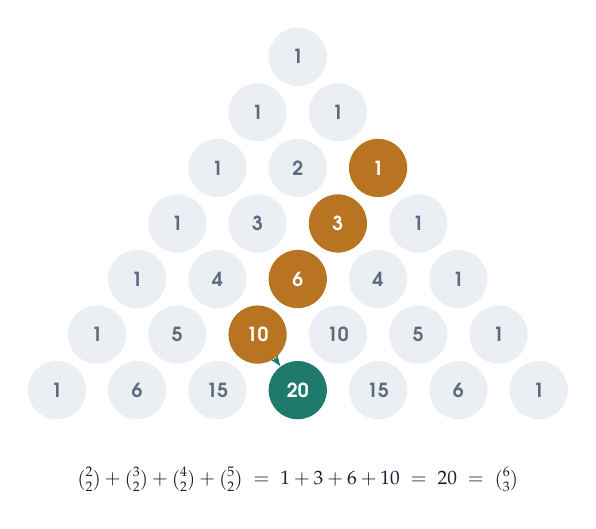
\begin{tikzpicture}[x=1.0cm,y=0.84cm]
\node[circle,fill=indigo!10,text=slate,inner sep=0pt,minimum size=7.4mm,font=\scriptsize\sffamily\bfseries] (h0-0) at (0.0,0.0) {1};
\node[circle,fill=indigo!10,text=slate,inner sep=0pt,minimum size=7.4mm,font=\scriptsize\sffamily\bfseries] (h1-0) at (-0.51,-0.84) {1};
\node[circle,fill=indigo!10,text=slate,inner sep=0pt,minimum size=7.4mm,font=\scriptsize\sffamily\bfseries] (h1-1) at (0.51,-0.84) {1};
\node[circle,fill=indigo!10,text=slate,inner sep=0pt,minimum size=7.4mm,font=\scriptsize\sffamily\bfseries] (h2-0) at (-1.02,-1.68) {1};
\node[circle,fill=indigo!10,text=slate,inner sep=0pt,minimum size=7.4mm,font=\scriptsize\sffamily\bfseries] (h2-1) at (0.0,-1.68) {2};
\node[circle,fill=amber,text=white,inner sep=0pt,minimum size=7.4mm,font=\scriptsize\sffamily\bfseries] (h2-2) at (1.02,-1.68) {1};
\node[circle,fill=indigo!10,text=slate,inner sep=0pt,minimum size=7.4mm,font=\scriptsize\sffamily\bfseries] (h3-0) at (-1.53,-2.52) {1};
\node[circle,fill=indigo!10,text=slate,inner sep=0pt,minimum size=7.4mm,font=\scriptsize\sffamily\bfseries] (h3-1) at (-0.51,-2.52) {3};
\node[circle,fill=amber,text=white,inner sep=0pt,minimum size=7.4mm,font=\scriptsize\sffamily\bfseries] (h3-2) at (0.51,-2.52) {3};
\node[circle,fill=indigo!10,text=slate,inner sep=0pt,minimum size=7.4mm,font=\scriptsize\sffamily\bfseries] (h3-3) at (1.53,-2.52) {1};
\node[circle,fill=indigo!10,text=slate,inner sep=0pt,minimum size=7.4mm,font=\scriptsize\sffamily\bfseries] (h4-0) at (-2.04,-3.36) {1};
\node[circle,fill=indigo!10,text=slate,inner sep=0pt,minimum size=7.4mm,font=\scriptsize\sffamily\bfseries] (h4-1) at (-1.02,-3.36) {4};
\node[circle,fill=amber,text=white,inner sep=0pt,minimum size=7.4mm,font=\scriptsize\sffamily\bfseries] (h4-2) at (0.0,-3.36) {6};
\node[circle,fill=indigo!10,text=slate,inner sep=0pt,minimum size=7.4mm,font=\scriptsize\sffamily\bfseries] (h4-3) at (1.02,-3.36) {4};
\node[circle,fill=indigo!10,text=slate,inner sep=0pt,minimum size=7.4mm,font=\scriptsize\sffamily\bfseries] (h4-4) at (2.04,-3.36) {1};
\node[circle,fill=indigo!10,text=slate,inner sep=0pt,minimum size=7.4mm,font=\scriptsize\sffamily\bfseries] (h5-0) at (-2.55,-4.2) {1};
\node[circle,fill=indigo!10,text=slate,inner sep=0pt,minimum size=7.4mm,font=\scriptsize\sffamily\bfseries] (h5-1) at (-1.53,-4.2) {5};
\node[circle,fill=amber,text=white,inner sep=0pt,minimum size=7.4mm,font=\scriptsize\sffamily\bfseries] (h5-2) at (-0.51,-4.2) {10};
\node[circle,fill=indigo!10,text=slate,inner sep=0pt,minimum size=7.4mm,font=\scriptsize\sffamily\bfseries] (h5-3) at (0.51,-4.2) {10};
\node[circle,fill=indigo!10,text=slate,inner sep=0pt,minimum size=7.4mm,font=\scriptsize\sffamily\bfseries] (h5-4) at (1.53,-4.2) {5};
\node[circle,fill=indigo!10,text=slate,inner sep=0pt,minimum size=7.4mm,font=\scriptsize\sffamily\bfseries] (h5-5) at (2.55,-4.2) {1};
\node[circle,fill=indigo!10,text=slate,inner sep=0pt,minimum size=7.4mm,font=\scriptsize\sffamily\bfseries] (h6-0) at (-3.06,-5.04) {1};
\node[circle,fill=indigo!10,text=slate,inner sep=0pt,minimum size=7.4mm,font=\scriptsize\sffamily\bfseries] (h6-1) at (-2.04,-5.04) {6};
\node[circle,fill=indigo!10,text=slate,inner sep=0pt,minimum size=7.4mm,font=\scriptsize\sffamily\bfseries] (h6-2) at (-1.02,-5.04) {15};
\node[circle,fill=teal,text=white,inner sep=0pt,minimum size=7.4mm,font=\scriptsize\sffamily\bfseries] (h6-3) at (0.0,-5.04) {20};
\node[circle,fill=indigo!10,text=slate,inner sep=0pt,minimum size=7.4mm,font=\scriptsize\sffamily\bfseries] (h6-4) at (1.02,-5.04) {15};
\node[circle,fill=indigo!10,text=slate,inner sep=0pt,minimum size=7.4mm,font=\scriptsize\sffamily\bfseries] (h6-5) at (2.04,-5.04) {6};
\node[circle,fill=indigo!10,text=slate,inner sep=0pt,minimum size=7.4mm,font=\scriptsize\sffamily\bfseries] (h6-6) at (3.06,-5.04) {1};
\draw[teal,line width=1.0pt,-{Stealth[length=4pt]}] (h5-2) -- (h6-3);
\node[font=\scriptsize\sffamily,color=ink,anchor=north] at (0,-6.05) {$\comb{2}{2}+\comb{3}{2}+\comb{4}{2}+\comb{5}{2}\;=\;1+3+6+10\;=\;20\;=\;\comb{6}{3}$};
\end{tikzpicture}
% ---- end fig-hockey.tex ----
\caption{The hockey stick: sum a diagonal, land one step down and across.}
\end{figure}

\begin{exbox}[Double counting in action: the sum of squares]
Choose $n$ people from a group of $n$ women and $n$ men. Directly this is
$\comb{2n}{n}$. Alternatively split on the number $k$ of women chosen: $\comb{n}{k}$
ways to pick the women, $\comb{n}{n-k}$ ways to pick the men, and $\comb{n}{n-k} =
\comb{n}{k}$ by symmetry. Summing over $k$:
\[
  \sum_{k=0}^{n}\comb{n}{k}^{2} \;=\; \comb{2n}{n}.
\]
Check at $n=3$: $1+9+9+1 = 20 = \comb{6}{3}$. \checkmark
\end{exbox}

\begin{warnbox}[Three habitual errors]
\begin{itemize}
  \item \textbf{Dividing twice.} If you already used $\comb{n}{k}$, the order is gone.
        Do not divide by $k!$ again.
  \item \textbf{Ordering identical groups.} Splitting $12$ people into three
        \emph{unlabelled} teams of $4$ is
        $\frac{1}{3!}\comb{12}{4}\comb{8}{4}\comb{4}{4}$, not
        $\comb{12}{4}\comb{8}{4}\comb{4}{4}$. If the teams have names (Red, Blue, Green),
        do \emph{not} divide.
  \item \textbf{Double-counting overlapping cases.} The sum rule requires
        \emph{disjoint} cases. ``Choose a committee containing Alice, or containing Bob''
        double-counts committees containing both. Use inclusion--exclusion
        (Section~\ref{sec:incexc}).
\end{itemize}
\end{warnbox}
% ---- end ch03-combinations.tex ----
% ---- begin ch04-binomial.tex ----
\section{The binomial theorem}

\begin{thmbox}[Binomial theorem]
For any commuting $x,y$ and any integer $n \ge 0$,
\[
  (x+y)^{n} \;=\; \sum_{k=0}^{n} \comb{n}{k}\, x^{\,n-k} y^{\,k}
  \;=\; x^n + n x^{n-1}y + \comb{n}{2}x^{n-2}y^2 + \dots + n x y^{n-1} + y^{n}.
\]
The general term is $T_{k+1} = \comb{n}{k}x^{\,n-k}y^{\,k}$, indexed so that
$T_1$ is the $x^n$ term.
\end{thmbox}

\begin{ideabox}[The theorem is a counting statement]
Write $(x+y)^n = \underbrace{(x+y)(x+y)\cdots(x+y)}_{n \text{ factors}}$ and expand by
choosing, from each factor, either the $x$ or the $y$. Every choice-sequence produces
one monomial. A monomial is $x^{n-k}y^k$ exactly when you chose $y$ from $k$ of the $n$
factors, and the number of ways to do that is $\comb{n}{k}$. So $\comb{n}{k}$ is the
coefficient. \emph{The binomial coefficient is called that because of this theorem.}
\end{ideabox}

\begin{exbox}[Extracting one coefficient]
Find the coefficient of $x^{7}$ in $\bigl(2x^{2} - \tfrac{3}{x}\bigr)^{8}$.

The general term is
\[
  T_{k+1} = \comb{8}{k}\,(2x^{2})^{8-k}\Bigl(-\frac{3}{x}\Bigr)^{k}
          = \comb{8}{k}\,2^{8-k}(-3)^{k}\,x^{16-2k-k}
          = \comb{8}{k}\,2^{8-k}(-3)^{k}\,x^{16-3k}.
\]
Set $16-3k = 7 \Rightarrow k = 3$. The coefficient is
\[
  \comb{8}{3}\,2^{5}\,(-3)^{3} = 56 \cdot 32 \cdot (-27) \ans{-48\,384}.
\]
\keyw{Method.} Always write the general term, collect the exponent of $x$ as a linear
function of $k$, and solve. If the equation has no non-negative integer solution
$0\le k\le n$, the coefficient is zero.
\end{exbox}

\subsection{Identities for free: substitute, then differentiate}

Because the theorem is an identity in $x$ and $y$, every substitution gives a new
identity, and so does every derivative.

\begin{thmbox}[Harvesting identities]
\begin{center}
\begin{tabularx}{\textwidth}{@{}lXl@{}}
\toprule
\textbf{Operation} & \textbf{Result} & \textbf{Value} \\
\midrule
$x=y=1$ & $\displaystyle\sum_{k}\comb{n}{k}$ & $2^{n}$ \\
$x=1,\;y=-1$ & $\displaystyle\sum_{k}(-1)^{k}\comb{n}{k}$ & $0$ \ ($n\ge 1$) \\
add the two & $\displaystyle\sum_{k \text{ even}}\comb{n}{k}$ & $2^{n-1}$ \ ($n\ge1$) \\
$x=1,\;y=2$ & $\displaystyle\sum_{k}\comb{n}{k}2^{k}$ & $3^{n}$ \\
$\dfrac{d}{dy}$ at $x=y=1$ & $\displaystyle\sum_{k}k\comb{n}{k}$ & $n\,2^{n-1}$ \\
$\dfrac{d^2}{dy^2}$ at $x=y=1$ & $\displaystyle\sum_{k}k(k-1)\comb{n}{k}$ & $n(n-1)2^{n-2}$ \\
\bottomrule
\end{tabularx}
\end{center}
\end{thmbox}

The last two are exactly the computations that will give you the mean and variance of
the binomial distribution in Section~\ref{sec:dists}. It is worth noticing now that
they are the same algebra.

\subsection{The shape of a row}

\begin{figure}[H]
\centering
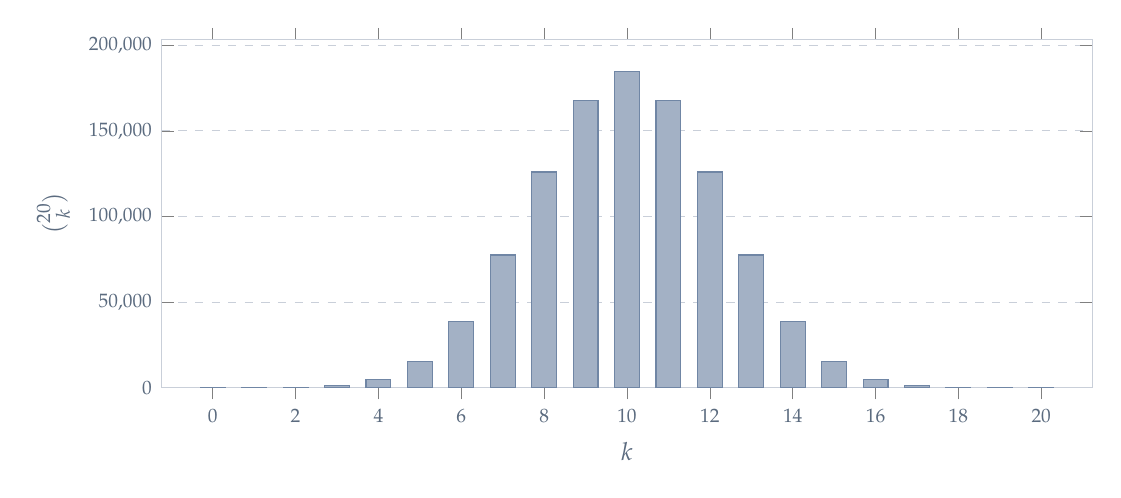
\begin{tikzpicture}
\begin{axis}[
  width=13.4cm, height=6.0cm,
  ybar, bar width=9pt,
  xlabel={$k$}, ylabel={$\comb{20}{k}$},
  xlabel style={font=\small\sffamily, color=slate},
  ylabel style={font=\small\sffamily, color=slate},
  tick label style={font=\scriptsize\sffamily, color=slate},
  axis line style={color=rule},
  ymajorgrids, grid style={color=rule, dashed, line width=0.4pt},
  xmin=-0.8, xmax=20.8, ymin=0,
  xtick={0,2,4,6,8,10,12,14,16,18,20},
  scaled y ticks=false, yticklabel style={/pgf/number format/fixed},
  enlarge x limits=0.02,
]
\addplot[draw=indigo!70, fill=indigo!45] coordinates {
 (0,1) (1,20) (2,190) (3,1140) (4,4845) (5,15504) (6,38760) (7,77520)
 (8,125970) (9,167960) (10,184756) (11,167960) (12,125970) (13,77520)
 (14,38760) (15,15504) (16,4845) (17,1140) (18,190) (19,20) (20,1)};
\end{axis}
\end{tikzpicture}
\caption{Row $n=20$ of Pascal's triangle. The row is symmetric, peaks at
$k=\lfloor n/2\rfloor$, and is already visibly bell-shaped. This is not a coincidence:
after dividing by $2^{n}$ it \emph{is} the $\mathrm{Bin}(20,\tfrac12)$ distribution,
and the de Moivre--Laplace theorem says it converges to a normal curve.}
\end{figure}

\begin{panel}[Where the row is largest]
$\comb{n}{k}$ increases in $k$ while $\dfrac{\comb{n}{k+1}}{\comb{n}{k}} = \dfrac{n-k}{k+1} > 1$,
that is while $k < \dfrac{n-1}{2}$. So the maximum is at $k=\lfloor n/2\rfloor$
(two equal maxima when $n$ is odd). The central coefficient satisfies
$\comb{2m}{m} \sim \dfrac{4^{m}}{\sqrt{\pi m}}$ by Stirling's formula,
$n! \sim \sqrt{2\pi n}\,(n/e)^{n}$.
\end{panel}

\subsection{The multinomial theorem}

\begin{thmbox}[Multinomial theorem]
\[
  (x_1 + x_2 + \dots + x_r)^{n}
  \;=\; \sum_{\substack{k_1+k_2+\dots+k_r=n \\ k_i \ge 0}}
        \binom{n}{k_1,\,k_2,\,\dots,\,k_r}\, x_1^{k_1}x_2^{k_2}\cdots x_r^{k_r},
\]
\[
  \text{where}\qquad
  \binom{n}{k_1,\dots,k_r} \;=\; \frac{n!}{k_1!\,k_2!\cdots k_r!}.
\]
The number of terms in the expansion is $\displaystyle\comb{n+r-1}{r-1}$
(see Section~\ref{sec:starsbars}), and setting every $x_i=1$ gives
$\displaystyle\sum \binom{n}{k_1,\dots,k_r} = r^{n}$.
\end{thmbox}

\begin{exbox}[A multinomial coefficient]
The coefficient of $x^{3}y^{2}z^{2}$ in $(x+y+z)^{7}$ is
\[
  \binom{7}{3,2,2} = \frac{7!}{3!\,2!\,2!} = \frac{5040}{24} \ans{210}.
\]
Same number as the arrangements of the multiset $\{x,x,x,y,y,z,z\}$, and for the same
reason: each term of the expansion \emph{is} such an arrangement.
\end{exbox}

\subsection{Beyond positive integer exponents}

\begin{thmbox}[Newton's generalised binomial series]
For any real $\alpha$ and $\lvert t\rvert < 1$,
\[
  (1+t)^{\alpha} \;=\; \sum_{k=0}^{\infty} \binom{\alpha}{k} t^{k},
  \qquad
  \binom{\alpha}{k} \eqdef \frac{\alpha(\alpha-1)\cdots(\alpha-k+1)}{k!}
  \;=\; \frac{\ffact{\alpha}{k}}{k!}.
\]
The falling-factorial definition is the one that survives; the factorial-quotient form
does not, because $\alpha!$ is meaningless for non-integers.
\end{thmbox}

Two consequences you will meet again:
\[
  \frac{1}{1-t} = \sum_{k\ge 0} t^{k},
  \qquad
  \frac{1}{(1-t)^{r}} = \sum_{k\ge 0} \comb{k+r-1}{r-1}\,t^{k}.
\]
The second is the generating function for stars and bars, which is the subject of the
next section, and for the negative binomial distribution later on.

\begin{warnbox}[Sign and index slips]
\begin{itemize}
  \item In $(x-y)^n$ the terms alternate: $\comb{n}{k}x^{n-k}(-y)^{k}$ carries $(-1)^k$.
        Fold the minus sign into $y$ \emph{before} expanding.
  \item $T_{k+1}$, not $T_k$, is the term with $y^{k}$. If a question asks for
        ``the $6$th term'', that is $k=5$.
  \item $\comb{n}{k}$ counts the $y$'s, so the exponent of $x$ is $n-k$. Check by
        confirming the exponents sum to $n$.
\end{itemize}
\end{warnbox}
% ---- end ch04-binomial.tex ----
% ---- begin ch05-starsbars.tex ----
\section{Stars and bars, and the master table}
\label{sec:starsbars}

Everything so far has been about \emph{selecting} without repetition. The remaining
case, unordered selection \emph{with} repetition, is the one people find hardest, and
it has a picture that makes it easy.

\begin{defbox}[The problem]
Count the solutions in non-negative integers of
\[
  x_1 + x_2 + \dots + x_r \;=\; n .
\]
Equivalently: the number of ways to distribute $n$ identical objects into $r$
distinguishable boxes; equivalently, the number of multisets of size $n$ drawn from
$r$ types.
\end{defbox}

\begin{ideabox}[The picture]
Draw the $n$ objects as \keyw{stars}. Insert $r-1$ \keyw{bars} to cut the row into $r$
compartments; the number of stars in compartment $i$ is $x_i$. Every arrangement of
$n$ stars and $r-1$ bars gives exactly one solution, and every solution gives exactly
one arrangement. So the two sets are in bijection, and we only have to count
arrangements of a row of $n+r-1$ symbols, of which $r-1$ are bars.
\end{ideabox}

\begin{figure}[H]
\centering
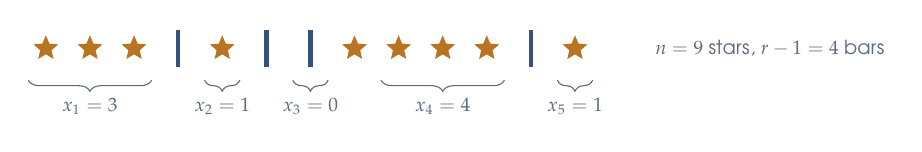
\begin{tikzpicture}[x=0.56cm,y=0.56cm]
  \def\syms{{"s","s","s","b","s","b","b","s","s","s","s","b","s"}}
  \foreach \i in {0,...,12}{
    \pgfmathparse{\syms[\i]}\edef\s{\pgfmathresult}
    \ifthenelse{\equal{\s}{s}}
      {\node[star, star points=5, star point ratio=2.2, fill=amber, draw=amber,
             inner sep=1.35pt] at (\i,0) {};}
      {\draw[indigo, line width=1.6pt] (\i,-0.42) -- (\i,0.42);}
  }
  \draw[decorate, decoration={brace, amplitude=4pt, mirror}, slate]
      (-0.4,-0.72) -- (2.4,-0.72) node[midway, below=3pt, font=\scriptsize\sffamily, color=slate] {$x_1=3$};
  \draw[decorate, decoration={brace, amplitude=4pt, mirror}, slate]
      (3.6,-0.72) -- (4.4,-0.72) node[midway, below=3pt, font=\scriptsize\sffamily, color=slate] {$x_2=1$};
  \draw[decorate, decoration={brace, amplitude=4pt, mirror}, slate]
      (5.6,-0.72) -- (6.4,-0.72) node[midway, below=3pt, font=\scriptsize\sffamily, color=slate] {$x_3=0$};
  \draw[decorate, decoration={brace, amplitude=4pt, mirror}, slate]
      (7.6,-0.72) -- (10.4,-0.72) node[midway, below=3pt, font=\scriptsize\sffamily, color=slate] {$x_4=4$};
  \draw[decorate, decoration={brace, amplitude=4pt, mirror}, slate]
      (11.6,-0.72) -- (12.4,-0.72) node[midway, below=3pt, font=\scriptsize\sffamily, color=slate] {$x_5=1$};
  \node[font=\scriptsize\sffamily, color=slate, anchor=west] at (13.6,0)
    {$n=9$ stars, $r-1=4$ bars};
\end{tikzpicture}
\caption{One arrangement of $9$ stars and $4$ bars, and the solution of
$x_1+\dots+x_5=9$ that it encodes. Choosing the solution is the same as choosing which
$4$ of the $13$ positions hold bars.}
\end{figure}

\begin{thmbox}[Stars and bars]
The number of non-negative integer solutions of $x_1+\dots+x_r = n$ is
\[
  \comb{n+r-1}{r-1} \;=\; \comb{n+r-1}{n}.
\]
The number of \emph{positive} integer solutions ($x_i \ge 1$) is
\[
  \comb{n-1}{r-1},
\]
obtained by substituting $y_i = x_i - 1 \ge 0$, which turns the equation into
$y_1+\dots+y_r = n-r$.
\end{thmbox}

\begin{exbox}[Two quick applications]
\textbf{(a)} How many ways to buy $12$ doughnuts from $5$ varieties, with unlimited
supply of each? This is $x_1+\dots+x_5=12$, so
$\comb{16}{4} = 1820$.

\medskip
\textbf{(b)} How many terms does $(a+b+c+d)^{10}$ have after collecting?
One term for each exponent vector with $k_1+k_2+k_3+k_4 = 10$, so
$\comb{13}{3} = 286$.
\end{exbox}

\begin{ideabox}[Lower bounds: shift. Upper bounds: inclusion--exclusion.]
A constraint $x_i \ge c$ costs nothing: substitute $x_i' = x_i - c$ and reduce $n$ by
$c$. A constraint $x_i \le c$ is genuinely harder, and is handled by subtracting the
bad cases (Section~\ref{sec:incexc}). For example, the solutions of
$x_1+x_2+x_3=15$ with every $x_i \le 8$:
\[
  \comb{17}{2} - \comb{3}{1}\comb{8}{2} + 0
  = 136 - 3\cdot 28 + 0 \ans{52},
\]
where the middle term subtracts, for each $i$, the solutions with $x_i \ge 9$ (shift by
$9$, leaving $x_1+x_2+x_3=6$, so $\comb{8}{2}=28$), and no two variables can both
exceed $8$ when the total is only $15$.
\end{ideabox}

\subsection{The master table}

Almost every elementary counting question is one of four questions. Choose $k$ items
from $n$ types; ask whether order matters, and whether repetition is allowed.

\begin{figure}[H]
\centering
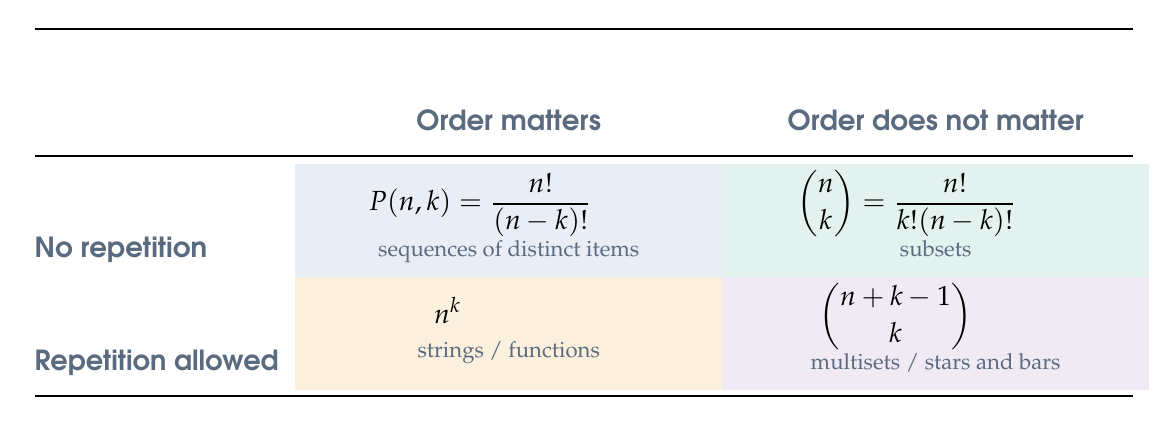
\begin{tikzpicture}[x=1cm,y=1cm]
  \node[anchor=north west, inner sep=0pt] at (0,0) {%
  \renewcommand{\arraystretch}{2.0}
  \begin{tabular}{@{}>{\sffamily\bfseries\color{slate}\raggedright}p{3.1cm}
                    >{\centering\arraybackslash}p{5.0cm}
                    >{\centering\arraybackslash}p{5.0cm}@{}}
   \toprule
   & \sffamily\bfseries\color{slate}Order matters
   & \sffamily\bfseries\color{slate}Order does not matter \\
   \midrule
   No repetition
     & \cellcolor{indigoLt}$\displaystyle \perm{n}{k}=\frac{n!}{(n-k)!}$
       \newline {\footnotesize\color{slate}sequences of distinct items}
     & \cellcolor{tealLt}$\displaystyle \comb{n}{k}=\frac{n!}{k!(n-k)!}$
       \newline {\footnotesize\color{slate}subsets} \\
   Repetition allowed
     & \cellcolor{amberLt}$\displaystyle n^{k}$
       \newline {\footnotesize\color{slate}strings / functions}
     & \cellcolor{plumLt}$\displaystyle \comb{n+k-1}{k}$
       \newline {\footnotesize\color{slate}multisets / stars and bars} \\
   \bottomrule
  \end{tabular}};
\end{tikzpicture}
\caption{The fourfold way. Identify the row and the column before you write a formula.}
\end{figure}

\begin{panel}[A fifth case that catches people out: partitions into groups]
Splitting a set is not the same as selecting from it.
\begin{itemize}
 \item \keyw{Ordered set partition into labelled groups of given sizes}
       $n_1,\dots,n_r$ summing to $n$: \quad
       $\displaystyle \binom{n}{n_1,\dots,n_r}=\frac{n!}{n_1!\cdots n_r!}$.
 \item \keyw{Unlabelled groups}, all of the same size $m$, with $r=n/m$ groups: divide by
       $r!$ \quad $\displaystyle \frac{n!}{(m!)^{r}\,r!}$.
 \item \keyw{Any number of unlabelled non-empty blocks}: the Bell number $B_n$;
       exactly $j$ blocks gives the Stirling number of the second kind $S(n,j)$, with
       $S(n,j)=j\,S(n-1,j)+S(n-1,j-1)$. These have no closed form as simple as
       $\comb{n}{k}$, which is why exam questions specify sizes.
\end{itemize}
\end{panel}
% ---- end ch05-starsbars.tex ----
% ---- begin ch06-inclusion.tex ----
\section{Inclusion--exclusion}
\label{sec:incexc}

The sum rule needs disjoint cases. When the cases overlap, you have to add the pieces,
subtract the double-counted overlaps, add back the triple-counted triple overlaps, and
so on. That alternating correction is inclusion--exclusion.

\begin{figure}[H]
\centering
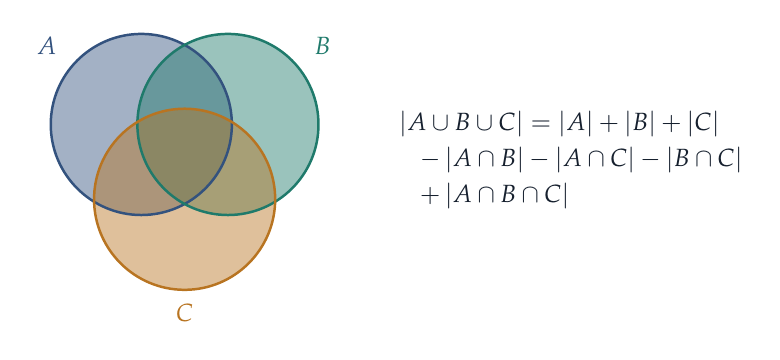
\begin{tikzpicture}[scale=1.0]
 \begin{scope}
  \begin{scope}[opacity=0.45]
    \fill[indigo] (-0.55,0.35) circle (1.15);
    \fill[teal]   ( 0.55,0.35) circle (1.15);
    \fill[amber]  ( 0.00,-0.6) circle (1.15);
  \end{scope}
  \draw[indigo, line width=0.9pt] (-0.55,0.35) circle (1.15);
  \draw[teal,   line width=0.9pt] ( 0.55,0.35) circle (1.15);
  \draw[amber,  line width=0.9pt] ( 0.00,-0.6) circle (1.15);
  \node[font=\small\sffamily\bfseries, color=indigo] at (-1.75,1.35) {$A$};
  \node[font=\small\sffamily\bfseries, color=teal]   at ( 1.75,1.35) {$B$};
  \node[font=\small\sffamily\bfseries, color=amber]  at ( 0.00,-2.05) {$C$};
 \end{scope}
 \node[font=\small\sffamily, color=ink, anchor=west, align=left] at (2.6,-0.1)
 {$\lvert A\cup B\cup C\rvert
   = \lvert A\rvert+\lvert B\rvert+\lvert C\rvert$\\[2pt]
   \hphantom{$=$}$-\,\lvert A\cap B\rvert-\lvert A\cap C\rvert-\lvert B\cap C\rvert$\\[2pt]
   \hphantom{$=$}$+\,\lvert A\cap B\cap C\rvert$};
\end{tikzpicture}
\caption{Each point of the union must be counted exactly once. A point in two discs is
added twice and subtracted once; a point in three discs is added three times,
subtracted three times, and added back once.}
\end{figure}

\begin{thmbox}[Inclusion--exclusion]
For finite sets $A_1,\dots,A_n$,
\[
  \Bigl\lvert \bigcup_{i=1}^{n} A_i \Bigr\rvert
  \;=\; \sum_{\emptyset \neq J \subseteq [n]} (-1)^{\lvert J\rvert+1}
        \Bigl\lvert \bigcap_{i \in J} A_i \Bigr\rvert
  \;=\; \sum_i \lvert A_i\rvert
        - \sum_{i<j}\lvert A_i \cap A_j\rvert
        + \sum_{i<j<k}\lvert A_i\cap A_j\cap A_k\rvert - \dots
\]
Equivalently, for the number of elements of a universe $S$ lying in \emph{none} of the
$A_i$:
\[
  \Bigl\lvert \bigcap_{i}\overline{A_i} \Bigr\rvert
  = \sum_{J \subseteq [n]} (-1)^{\lvert J\rvert}\Bigl\lvert \bigcap_{i\in J}A_i\Bigr\rvert ,
  \qquad \text{with } \bigcap_{i \in \emptyset} A_i = S .
\]
The identical statement for probabilities holds with $\lvert\cdot\rvert$ replaced by
$\Prob(\cdot)$.
\end{thmbox}

\begin{ideabox}[Why the signs alternate]
Take an element lying in exactly $m \ge 1$ of the sets. On the right-hand side it is
counted once for every non-empty subset of those $m$ sets, with sign
$(-1)^{\lvert J\rvert +1}$, contributing
\[
  \sum_{j=1}^{m}(-1)^{j+1}\comb{m}{j} \;=\; 1 - \sum_{j=0}^{m}(-1)^{j}\comb{m}{j} \;=\; 1-0 \;=\; 1 .
\]
The alternating row sum of Pascal's triangle is exactly what makes the bookkeeping come
out right. Elements in none of the sets contribute $0$. So the right-hand side counts
each element of the union once.
\end{ideabox}

\begin{exbox}[Surjections]
How many functions from a $6$-set onto a $3$-set (that is, hitting every target)?
Let $A_i$ be the set of functions missing target $i$. Then
\[
  \#\text{surjections} = 3^{6} - \comb{3}{1}2^{6} + \comb{3}{2}1^{6} - \comb{3}{3}0^{6}
  = 729 - 192 + 3 - 0 \ans{540}.
\]
In general the number of surjections $[n] \twoheadrightarrow [r]$ is
$\displaystyle \sum_{j=0}^{r}(-1)^{j}\comb{r}{j}(r-j)^{n} = r!\,S(n,r)$.
\end{exbox}

\subsection{Derangements}

\begin{defbox}[Derangement]
A \keyw{derangement} of $[n]$ is a permutation with no fixed point: $\sigma(i)\neq i$
for every $i$. Write $D_n$ (also $!n$) for the number of them.
\end{defbox}

\begin{thmbox}[Count and asymptotics]
Let $A_i$ be the permutations fixing $i$, so $\lvert \bigcap_{i \in J} A_i\rvert
= (n-\lvert J\rvert)!$. Inclusion--exclusion gives
\[
  D_n \;=\; \sum_{j=0}^{n}(-1)^{j}\comb{n}{j}(n-j)!
        \;=\; n!\sum_{j=0}^{n}\frac{(-1)^{j}}{j!}
        \;=\; \left\lfloor \frac{n!}{e} + \frac12 \right\rfloor \ (n\ge 1),
\]
with the recurrences $D_n = (n-1)(D_{n-1}+D_{n-2})$ and $D_n = nD_{n-1}+(-1)^n$.
Hence
\[
  \frac{D_n}{n!} \;\longrightarrow\; e^{-1} \approx 0.3679 .
\]
\end{thmbox}

\begin{figure}[H]
\centering
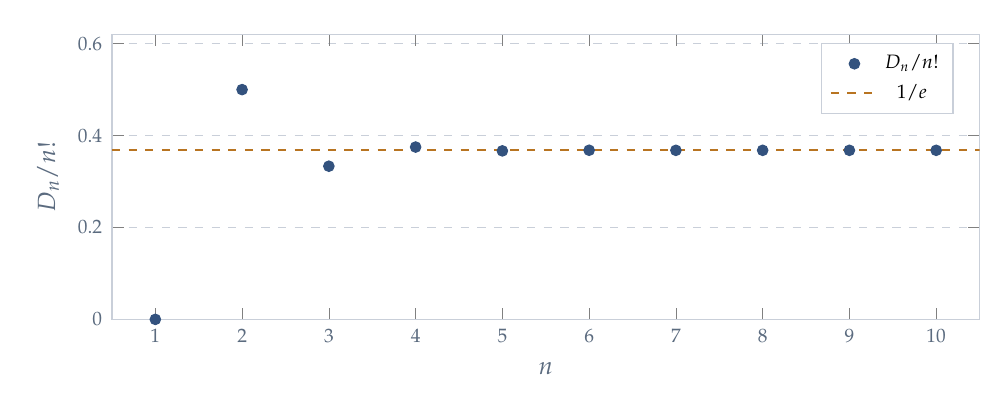
\begin{tikzpicture}
\begin{axis}[
  width=12.6cm, height=5.2cm,
  xlabel={$n$}, ylabel={$D_n/n!$},
  xlabel style={font=\small\sffamily, color=slate},
  ylabel style={font=\small\sffamily, color=slate},
  tick label style={font=\scriptsize\sffamily, color=slate},
  axis line style={color=rule},
  ymajorgrids, grid style={color=rule, dashed, line width=0.4pt},
  xmin=0.5, xmax=10.5, ymin=0, ymax=0.62,
  xtick={1,2,3,4,5,6,7,8,9,10},
  legend style={font=\scriptsize\sffamily, draw=rule, fill=white},
  legend pos=north east,
]
\addplot[only marks, mark=*, mark size=1.9pt, color=indigo] coordinates {
 (1,0) (2,0.5) (3,0.333333) (4,0.375) (5,0.366667) (6,0.368056)
 (7,0.367857) (8,0.367882) (9,0.367879) (10,0.367879)};
\addlegendentry{$D_n/n!$}
\addplot[domain=0.5:10.5, samples=2, color=amber, thick, dashed] {0.3678794};
\addlegendentry{$1/e$}
\end{axis}
\end{tikzpicture}
\caption{The proportion of derangements settles onto $1/e$ almost immediately: the
error is smaller than $1/(n+1)!$, so by $n=7$ it is already correct to five decimals.}
\end{figure}

\begin{exbox}[The hat-check problem]
Ten people check their hats and receive them back at random. The probability that
\emph{nobody} gets their own hat is $D_{10}/10! \approx 0.3679$. The probability that
\emph{exactly $k$} people get their own hat is
\[
  \Prob(\text{exactly } k) = \frac{\comb{n}{k}D_{n-k}}{n!} \approx \frac{e^{-1}}{k!},
\]
which is $\mathrm{Poisson}(1)$ in the limit. The expected number of fixed points is
exactly $1$ for every $n \ge 1$, by linearity of expectation
(Section~\ref{sec:expectation}).
\end{exbox}

\begin{panel}[When to reach for inclusion--exclusion]
Look for the words \emph{at least one}, \emph{none}, \emph{no two}, or a list of
forbidden patterns. Define $A_i$ = ``constraint $i$ is violated'', count intersections
(which are usually easy, because forcing several constraints to fail typically just
shrinks the problem), and alternate. If the intersections are hard to count, the method
is the wrong tool.
\end{panel}
% ---- end ch06-inclusion.tex ----
% ---- begin ch07-bijections.tex ----
\section{Bijections: counting by disguise}
\label{sec:bijections}

The best counting arguments do not compute anything. They show that the set you care
about is secretly a set you already know how to count.

\subsection{Lattice paths}

\begin{thmbox}[Monotone lattice paths]
The number of paths from $(0,0)$ to $(m,n)$ using only unit steps right
(\texttt{R}) and up (\texttt{U}) is
\[
  \comb{m+n}{n} \;=\; \comb{m+n}{m}.
\]
\textbf{Proof.} A path is a word of $m+n$ letters, $m$ of them \texttt{R} and $n$ of
them \texttt{U}. Choosing the path is choosing which $n$ of the $m+n$ positions are
\texttt{U}. \qed
\end{thmbox}

\begin{figure}[H]
\centering
% ---- begin fig-lattice.tex ----
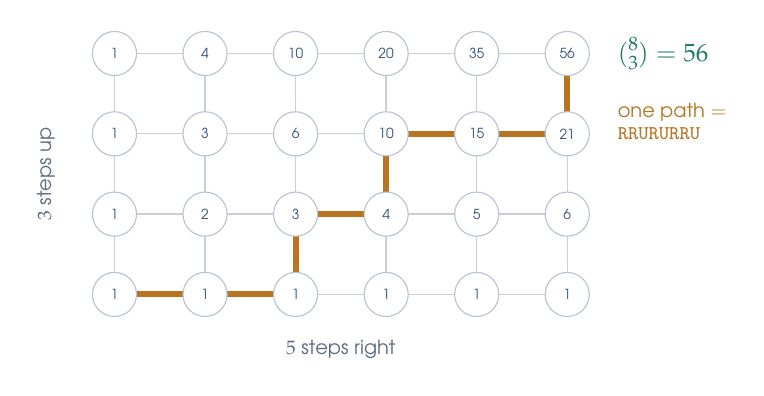
\begin{tikzpicture}[x=1.15cm,y=1.02cm]
\draw[rule,line width=0.5pt] (0,0) -- (0,3);
\draw[rule,line width=0.5pt] (1,0) -- (1,3);
\draw[rule,line width=0.5pt] (2,0) -- (2,3);
\draw[rule,line width=0.5pt] (3,0) -- (3,3);
\draw[rule,line width=0.5pt] (4,0) -- (4,3);
\draw[rule,line width=0.5pt] (5,0) -- (5,3);
\draw[rule,line width=0.5pt] (0,0) -- (5,0);
\draw[rule,line width=0.5pt] (0,1) -- (5,1);
\draw[rule,line width=0.5pt] (0,2) -- (5,2);
\draw[rule,line width=0.5pt] (0,3) -- (5,3);
\draw[amber,line width=2.2pt,line cap=round,line join=round] (0,0) -- (1,0) -- (2,0) -- (2,1) -- (3,1) -- (3,2) -- (4,2) -- (5,2) -- (5,3);
\node[circle,fill=white,draw=indigo!35,inner sep=0pt,minimum size=5.6mm,font=\tiny\sffamily,text=indigo] at (0,0) {1};
\node[circle,fill=white,draw=indigo!35,inner sep=0pt,minimum size=5.6mm,font=\tiny\sffamily,text=indigo] at (0,1) {1};
\node[circle,fill=white,draw=indigo!35,inner sep=0pt,minimum size=5.6mm,font=\tiny\sffamily,text=indigo] at (0,2) {1};
\node[circle,fill=white,draw=indigo!35,inner sep=0pt,minimum size=5.6mm,font=\tiny\sffamily,text=indigo] at (0,3) {1};
\node[circle,fill=white,draw=indigo!35,inner sep=0pt,minimum size=5.6mm,font=\tiny\sffamily,text=indigo] at (1,0) {1};
\node[circle,fill=white,draw=indigo!35,inner sep=0pt,minimum size=5.6mm,font=\tiny\sffamily,text=indigo] at (1,1) {2};
\node[circle,fill=white,draw=indigo!35,inner sep=0pt,minimum size=5.6mm,font=\tiny\sffamily,text=indigo] at (1,2) {3};
\node[circle,fill=white,draw=indigo!35,inner sep=0pt,minimum size=5.6mm,font=\tiny\sffamily,text=indigo] at (1,3) {4};
\node[circle,fill=white,draw=indigo!35,inner sep=0pt,minimum size=5.6mm,font=\tiny\sffamily,text=indigo] at (2,0) {1};
\node[circle,fill=white,draw=indigo!35,inner sep=0pt,minimum size=5.6mm,font=\tiny\sffamily,text=indigo] at (2,1) {3};
\node[circle,fill=white,draw=indigo!35,inner sep=0pt,minimum size=5.6mm,font=\tiny\sffamily,text=indigo] at (2,2) {6};
\node[circle,fill=white,draw=indigo!35,inner sep=0pt,minimum size=5.6mm,font=\tiny\sffamily,text=indigo] at (2,3) {10};
\node[circle,fill=white,draw=indigo!35,inner sep=0pt,minimum size=5.6mm,font=\tiny\sffamily,text=indigo] at (3,0) {1};
\node[circle,fill=white,draw=indigo!35,inner sep=0pt,minimum size=5.6mm,font=\tiny\sffamily,text=indigo] at (3,1) {4};
\node[circle,fill=white,draw=indigo!35,inner sep=0pt,minimum size=5.6mm,font=\tiny\sffamily,text=indigo] at (3,2) {10};
\node[circle,fill=white,draw=indigo!35,inner sep=0pt,minimum size=5.6mm,font=\tiny\sffamily,text=indigo] at (3,3) {20};
\node[circle,fill=white,draw=indigo!35,inner sep=0pt,minimum size=5.6mm,font=\tiny\sffamily,text=indigo] at (4,0) {1};
\node[circle,fill=white,draw=indigo!35,inner sep=0pt,minimum size=5.6mm,font=\tiny\sffamily,text=indigo] at (4,1) {5};
\node[circle,fill=white,draw=indigo!35,inner sep=0pt,minimum size=5.6mm,font=\tiny\sffamily,text=indigo] at (4,2) {15};
\node[circle,fill=white,draw=indigo!35,inner sep=0pt,minimum size=5.6mm,font=\tiny\sffamily,text=indigo] at (4,3) {35};
\node[circle,fill=white,draw=indigo!35,inner sep=0pt,minimum size=5.6mm,font=\tiny\sffamily,text=indigo] at (5,0) {1};
\node[circle,fill=white,draw=indigo!35,inner sep=0pt,minimum size=5.6mm,font=\tiny\sffamily,text=indigo] at (5,1) {6};
\node[circle,fill=white,draw=indigo!35,inner sep=0pt,minimum size=5.6mm,font=\tiny\sffamily,text=indigo] at (5,2) {21};
\node[circle,fill=white,draw=indigo!35,inner sep=0pt,minimum size=5.6mm,font=\tiny\sffamily,text=indigo] at (5,3) {56};
\node[font=\scriptsize\sffamily,color=slate,anchor=north] at (2.5,-0.45) {$5$ steps right};
\node[font=\scriptsize\sffamily,color=slate,anchor=south,rotate=90] at (-0.55,1.5) {$3$ steps up};
\node[font=\small\sffamily,color=teal,anchor=west] at (5.45,3) {$\comb{8}{3}=56$};
\node[font=\scriptsize\sffamily,color=amber,anchor=west,align=left] at (5.45,2.15) {one path $=$\\ \texttt{RRURURRU}};
\end{tikzpicture}
% ---- end fig-lattice.tex ----
\caption{Every vertex is labelled with the number of paths reaching it from the
origin. The labels satisfy Pascal's rule, because a path arrives at a vertex either
from the left or from below: Pascal's triangle \emph{is} the lattice-path count, tilted.}
\end{figure}

This one bijection explains several formulas at once. A path is a binary string; a
binary string is a subset; a subset is a $0/1$ vector; a $0/1$ vector with prescribed
weight is a combination. Any question about one of them can be moved to whichever
representation makes it easiest.

\subsection{The reflection principle and the ballot problem}

\begin{ideabox}[Reflect the bad paths]
To count paths that \emph{avoid} a forbidden line, count all paths and subtract the bad
ones. The bad ones are counted by reflecting the portion of the path before its first
touch of the line: this maps bad paths bijectively onto \emph{all} paths from the
reflected starting point, and those are unconstrained, so easy to count.
\end{ideabox}

\begin{figure}[H]
\centering
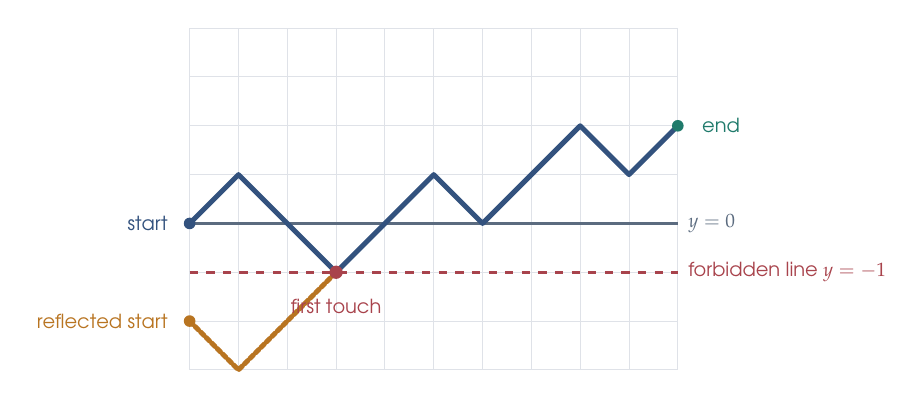
\begin{tikzpicture}[x=0.62cm,y=0.62cm]
  \draw[rule!60, line width=0.35pt, step=0.62cm] (0,-3) grid (10,4);
  \draw[slate, line width=0.9pt] (0,0) -- (10,0) node[right, font=\scriptsize\sffamily, color=slate] {$y=0$};
  \draw[rose, line width=1.0pt, dashed] (0,-1) -- (10,-1)
        node[right, font=\scriptsize\sffamily, color=rose] {forbidden line $y=-1$};
  % original bad path
  \draw[indigo, line width=1.8pt, line cap=round, line join=round]
    (0,0) -- (1,1) -- (2,0) -- (3,-1) -- (4,0) -- (5,1) -- (6,0) -- (7,1) -- (8,2) -- (9,1) -- (10,2);
  % reflected prefix
  \draw[amber, line width=1.8pt, line cap=round, line join=round, densely dotted]
    (0,-2) -- (1,-3) -- (2,-2) -- (3,-1);
  \fill[indigo] (0,0) circle (2.1pt);
  \fill[amber]  (0,-2) circle (2.1pt);
  \fill[teal]   (10,2) circle (2.1pt);
  \node[font=\scriptsize\sffamily, color=indigo, anchor=east] at (-0.25,0) {start};
  \node[font=\scriptsize\sffamily, color=amber, anchor=east] at (-0.25,-2) {reflected start};
  \node[font=\scriptsize\sffamily, color=teal, anchor=west] at (10.3,2) {end};
  \fill[rose] (3,-1) circle (2.4pt);
  \node[font=\scriptsize\sffamily, color=rose, anchor=north] at (3,-1.35) {first touch};
\end{tikzpicture}
\caption{Reflection. The path segment before the first touch of the forbidden line is
mirrored in that line. Bad paths from the true start correspond one-to-one with
\emph{all} paths from the mirrored start.}
\end{figure}

\begin{thmbox}[Bertrand's ballot problem]
Candidate $A$ receives $a$ votes and candidate $B$ receives $b$ votes, with $a>b$.
If the ballots are counted in a uniformly random order, the probability that $A$ is
strictly ahead throughout the count is
\[
  \frac{a-b}{a+b}.
\]
\end{thmbox}

\subsection{Catalan numbers}

\begin{defbox}[Catalan number]
\[
  C_n \;=\; \frac{1}{n+1}\comb{2n}{n} \;=\; \comb{2n}{n}-\comb{2n}{n+1},
\]
\[
  C_0,C_1,C_2,\dots \;=\; 1,\,1,\,2,\,5,\,14,\,42,\,132,\,429,\,1430,\,4862,\dots
\]
with the recurrence $C_{n+1} = \sum_{i=0}^{n} C_i C_{n-i}$ and growth
$C_n \sim \dfrac{4^{n}}{n^{3/2}\sqrt{\pi}}$.
\end{defbox}

$C_n$ counts, among many hundreds of other things:

\begin{itemize}
  \item balanced strings of $n$ pairs of parentheses;
  \item monotone lattice paths from $(0,0)$ to $(n,n)$ that never rise above the
        diagonal (\keyw{Dyck paths});
  \item binary trees with $n$ internal nodes;
  \item triangulations of a convex $(n+2)$-gon;
  \item ways to stack coins in a row of $n$ touching coins;
  \item sequences of $n$ pushes and $n$ pops of a stack that never pop an empty stack.
\end{itemize}

\begin{ideabox}[Why $\tfrac{1}{n+1}\comb{2n}{n}$]
Of the $\comb{2n}{n}$ paths from $(0,0)$ to $(n,n)$, the bad ones cross the diagonal.
Reflect a bad path in the line $y=x+1$ after its first crossing: the endpoint $(n,n)$
becomes $(n-1,n+1)$, and this is a bijection between bad paths and \emph{all} paths to
$(n-1,n+1)$, of which there are $\comb{2n}{n+1}$. Hence
\[
  C_n = \comb{2n}{n} - \comb{2n}{n+1}
      = \comb{2n}{n}\left(1 - \frac{n}{n+1}\right)
      = \frac{1}{n+1}\comb{2n}{n}.
\]
\end{ideabox}

\begin{figure}[H]
\centering
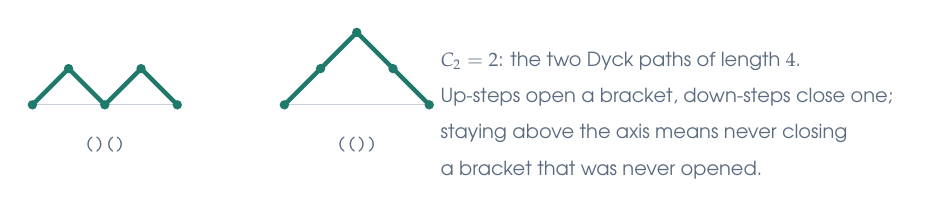
\begin{tikzpicture}[x=0.46cm,y=0.46cm]
  \begin{scope}
    \draw[rule, line width=0.4pt] (0,0) -- (4,0);
    \draw[teal, line width=1.6pt, line cap=round, line join=round]
      (0,0) -- (1,1) -- (2,0) -- (3,1) -- (4,0);
    \foreach \x/\y in {0/0,1/1,2/0,3/1,4/0}{\fill[teal] (\x,\y) circle (1.7pt);}
    \node[font=\scriptsize\ttfamily, color=slate] at (2,-1.1) {()()};
  \end{scope}
  \begin{scope}[xshift=3.2cm]
    \draw[rule, line width=0.4pt] (0,0) -- (4,0);
    \draw[teal, line width=1.6pt, line cap=round, line join=round]
      (0,0) -- (1,1) -- (2,2) -- (3,1) -- (4,0);
    \foreach \x/\y in {0/0,1/1,2/2,3/1,4/0}{\fill[teal] (\x,\y) circle (1.7pt);}
    \node[font=\scriptsize\ttfamily, color=slate] at (2,-1.1) {(())};
  \end{scope}
  \node[font=\scriptsize\sffamily, color=slate, anchor=west] at (11.0,1.2)
    {$C_2 = 2$: the two Dyck paths of length $4$.};
  \node[font=\scriptsize\sffamily, color=slate, anchor=west] at (11.0,0.2)
    {Up-steps open a bracket, down-steps close one;};
  \node[font=\scriptsize\sffamily, color=slate, anchor=west] at (11.0,-0.8)
    {staying above the axis means never closing};
  \node[font=\scriptsize\sffamily, color=slate, anchor=west] at (11.0,-1.8)
    {a bracket that was never opened.};
\end{tikzpicture}
\caption{Dyck paths never dip below the axis. Up-steps are open brackets, down-steps
are close brackets.}
\end{figure}

\begin{panel}[A checklist for building a bijection]
\begin{enumerate}
  \item Describe an element of your set as a \emph{string of decisions}.
  \item Check that different elements give different strings (injective).
  \item Check that every legal string comes from an element (surjective).
  \item Count the strings.
\end{enumerate}
Steps 2 and 3 are the proof; skipping them is how overcounting sneaks back in.
\end{panel}
% ---- end ch07-bijections.tex ----
\clearpage
\part{Probability}
% ---- begin ch08-axioms.tex ----
\section{From counting to probability}

\begin{defbox}[Sample space, event, probability measure]
A \keyw{sample space} $S$ is the set of possible outcomes of an experiment. An
\keyw{event} is a subset $A \subseteq S$. A \keyw{probability measure} assigns to each
event a number $\Prob(A)$ satisfying \keyw{Kolmogorov's axioms}:
\begin{enumerate}[label=\textbf{A\arabic*.}]
  \item $\Prob(A) \ge 0$ for every event $A$;
  \item $\Prob(S) = 1$;
  \item if $A_1, A_2, \dots$ are pairwise disjoint then
        $\Prob\bigl(\bigcup_i A_i\bigr) = \sum_i \Prob(A_i)$.
\end{enumerate}
\end{defbox}

Axiom A3 is the sum rule again. Everything below follows from these three lines alone.

\begin{thmbox}[Consequences]
\begin{center}
\begin{tabularx}{\textwidth}{@{}lX@{}}
\toprule
Complement & $\Prob(\overline{A}) = 1-\Prob(A)$, and $\Prob(\emptyset)=0$ \\
Monotonicity & $A \subseteq B \Rightarrow \Prob(A) \le \Prob(B)$, so $\Prob(A)\le 1$ \\
Two events & $\Prob(A\cup B) = \Prob(A)+\Prob(B)-\Prob(A\cap B)$ \\
Union bound & $\Prob\bigl(\bigcup_i A_i\bigr) \le \sum_i \Prob(A_i)$ \\
Inclusion--exclusion & $\Prob\bigl(\bigcup_{i=1}^{n} A_i\bigr)
   = \sum_{\emptyset\neq J\subseteq[n]}(-1)^{\lvert J\rvert+1}\Prob\bigl(\bigcap_{i\in J}A_i\bigr)$ \\
Partition & if $B_1,\dots,B_m$ partition $S$ then $\Prob(A) = \sum_j \Prob(A \cap B_j)$ \\
\bottomrule
\end{tabularx}
\end{center}
\end{thmbox}

\begin{defbox}[The equally likely (classical) model]
If $S$ is finite and every outcome is equally likely, then for every event $A$
\[
  \Prob(A) \;=\; \frac{\lvert A\rvert}{\lvert S\rvert}.
\]
\end{defbox}

\begin{warnbox}[The model is a choice, not a fact]
``Equally likely'' is an assumption you impose on the sample space, and you can make it
true or false by choosing the sample space badly. If you model two coin flips by
$S = \{\text{0 heads},\ \text{1 head},\ \text{2 heads}\}$ and assume equal likelihood,
you get $\Prob(\text{2 heads}) = 1/3$, which is wrong. Model with
$S = \{HH, HT, TH, TT\}$ instead. \keyw{Rule.} Build the sample space out of the
\emph{physical symmetries} of the experiment (individual coins, individual cards,
individual people), never out of summary statistics.
\end{warnbox}

\subsection{A worked catalogue: five-card poker hands}

There are $\comb{52}{5} = 2\,598\,960$ equally likely hands. Each row below is a pure
counting exercise, and together they are a good test of whether the fourfold way has
sunk in.

\begin{table}[H]
\centering
{\small
\begin{tabular}{@{}lllrl@{}}
\toprule
\sffamily\bfseries\color{slate}Hand & \sffamily\bfseries\color{slate}Count, as a product
 & \sffamily\bfseries\color{slate}Number & \sffamily\bfseries\color{slate}Probability
 & \sffamily\bfseries\color{slate}Odds \\
\midrule
Straight flush & $10\cdot 4$ & $40$ & $0.000015$ & $1$ in $64\,974$ \\
Four of a kind & $13\cdot 48$ & $624$ & $0.000240$ & $1$ in $4\,165$ \\
Full house & $13\comb{4}{3}\cdot 12\comb{4}{2}$ & $3\,744$ & $0.001441$ & $1$ in $694$ \\
Flush (not straight) & $4\comb{13}{5}-40$ & $5\,108$ & $0.001965$ & $1$ in $509$ \\
Straight (not flush) & $10\cdot 4^{5}-40$ & $10\,200$ & $0.003925$ & $1$ in $255$ \\
Three of a kind & $13\comb{4}{3}\comb{12}{2}4^{2}$ & $54\,912$ & $0.021128$ & $1$ in $47$ \\
Two pair & $\comb{13}{2}\comb{4}{2}^{2}\cdot 44$ & $123\,552$ & $0.047539$ & $1$ in $21$ \\
One pair & $13\comb{4}{2}\comb{12}{3}4^{3}$ & $1\,098\,240$ & $0.422569$ & $1$ in $2$ \\
High card (nothing) & remainder & $1\,302\,540$ & $0.501177$ & $1$ in $2$ \\
\midrule
\textbf{Total} & & $2\,598\,960$ & $1.000000$ & \\
\bottomrule
\end{tabular}}
\caption{The counts sum exactly to $\comb{52}{5}$, which is the check that the case
split was disjoint and exhaustive.}
\end{table}

\begin{ideabox}[How to read the products]
\emph{Full house.} Choose the rank that appears three times ($13$), choose which three
of its four suits ($\comb{4}{3}$), choose the rank appearing twice ($12$, not $13$:
it must differ), choose its two suits ($\comb{4}{2}$).

\emph{Two pair.} Choose the two pair-ranks together ($\comb{13}{2}$, unordered, because
naming them in the other order gives the same hand), suits for each
($\comb{4}{2}^2$), then the fifth card from the $44$ cards of the remaining $11$ ranks.

\emph{The $-40$.} Straights and flushes overlap in the $40$ straight flushes, so each
category must exclude them to keep the cases disjoint.
\end{ideabox}

\begin{exbox}[Complement, again]
What is the probability that a five-card hand contains at least one ace?
\[
  1 - \frac{\comb{48}{5}}{\comb{52}{5}} = 1 - \frac{1\,712\,304}{2\,598\,960}
  \approx \ans{0.3412}.
\]
Note that $\comb{4}{1}\comb{48}{4}/\comb{52}{5} \approx 0.2995$ is the probability of
\emph{exactly} one ace, which is a different question. And the tempting shortcut
``choose an ace, then any four other cards'',
$\comb{4}{1}\comb{51}{4}/\comb{52}{5} \approx 0.3846$, is simply wrong: a hand with two
aces is produced twice, once for each ace that could have been the designated one.
\end{exbox}
% ---- end ch08-axioms.tex ----
% ---- begin ch09-conditional.tex ----
\section{Conditional probability and Bayes}
\label{sec:conditional}

\begin{defbox}[Conditional probability]
For events $A,B$ with $\Prob(B)>0$,
\[
  \Prob(A \given B) \;\eqdef\; \frac{\Prob(A\cap B)}{\Prob(B)} .
\]
Conditioning on $B$ is a change of universe: $B$ becomes the new sample space, and all
probabilities are renormalised by $\Prob(B)$ so they sum to $1$ again. In the
equally-likely model this is just
$\Prob(A\given B) = \lvert A\cap B\rvert / \lvert B\rvert$: counting inside $B$.
\end{defbox}

\begin{thmbox}[The rules that follow]
\begin{align*}
\text{Multiplication rule:}\quad & \Prob(A\cap B) = \Prob(B)\,\Prob(A\given B) = \Prob(A)\,\Prob(B \given A) \\[2pt]
\text{Chain rule:}\quad & \Prob(A_1\cap\dots\cap A_n) = \Prob(A_1)\Prob(A_2\given A_1)\cdots\Prob(A_n \given A_1\cap\dots\cap A_{n-1}) \\[2pt]
\text{Total probability:}\quad & \Prob(A) = \sum_{j}\Prob(B_j)\,\Prob(A\given B_j)
   \quad\text{for any partition } \{B_j\} \text{ of } S \\[2pt]
\text{Bayes:}\quad & \Prob(B_i \given A) = \frac{\Prob(B_i)\,\Prob(A\given B_i)}{\sum_j \Prob(B_j)\,\Prob(A\given B_j)}
\end{align*}
\end{thmbox}

\begin{figure}[H]
\centering
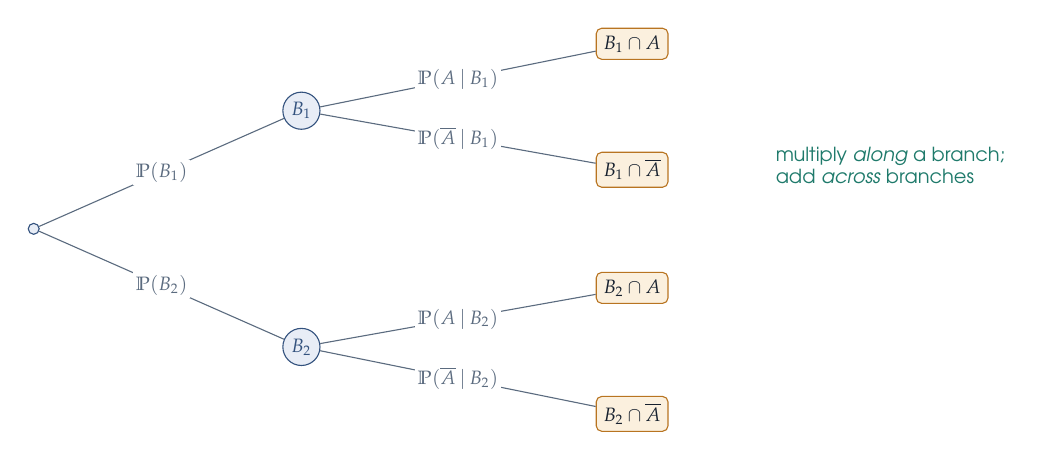
\begin{tikzpicture}[
  grow=right, level distance=30mm, sibling distance=13mm,
  every node/.style={font=\small\sffamily},
  edgelab/.style={font=\scriptsize\sffamily, color=slate, midway, fill=white, inner sep=1pt},
  nd/.style={circle, draw=indigo, fill=indigoLt, inner sep=1.4pt, font=\scriptsize\sffamily, text=indigo},
  lf/.style={rectangle, rounded corners=2pt, draw=amber, fill=amberLt, inner sep=2.6pt,
             font=\scriptsize\sffamily, text=ink}
]
\node[nd] (r) at (0,0) {};
\node[nd] (b1) at (3.4, 1.5) {$B_1$};
\node[nd] (b2) at (3.4,-1.5) {$B_2$};
\draw[slate] (r) -- node[edgelab] {$\Prob(B_1)$} (b1);
\draw[slate] (r) -- node[edgelab] {$\Prob(B_2)$} (b2);
\node[lf] (a1) at (7.6, 2.35) {$B_1\cap A$};
\node[lf] (a2) at (7.6, 0.75) {$B_1\cap \overline{A}$};
\node[lf] (a3) at (7.6,-0.75) {$B_2\cap A$};
\node[lf] (a4) at (7.6,-2.35) {$B_2\cap \overline{A}$};
\draw[slate] (b1) -- node[edgelab] {$\Prob(A\given B_1)$} (a1);
\draw[slate] (b1) -- node[edgelab] {$\Prob(\overline{A}\given B_1)$} (a2);
\draw[slate] (b2) -- node[edgelab] {$\Prob(A\given B_2)$} (a3);
\draw[slate] (b2) -- node[edgelab] {$\Prob(\overline{A}\given B_2)$} (a4);
\node[font=\scriptsize\sffamily, color=teal, anchor=west, align=left] at (9.3,0.8)
  {multiply \emph{along} a branch;\\ add \emph{across} branches};
\end{tikzpicture}
\caption{The probability tree. $\Prob(A)$ is the sum of the two amber leaves containing
$A$; $\Prob(B_1 \given A)$ is the top leaf divided by that sum. Bayes' theorem is
nothing more than this picture read backwards.}
\end{figure}

\begin{defbox}[Independence]
$A$ and $B$ are \keyw{independent} iff $\Prob(A\cap B) = \Prob(A)\Prob(B)$, equivalently
$\Prob(A\given B)=\Prob(A)$ when $\Prob(B)>0$. Events $A_1,\dots,A_n$ are
\keyw{mutually independent} iff for \emph{every} subset $J$,
$\Prob\bigl(\bigcap_{i\in J}A_i\bigr) = \prod_{i \in J}\Prob(A_i)$.
\end{defbox}

\begin{warnbox}[Independence is not pairwise independence, and is not disjointness]
\textbf{Pairwise is weaker.} Toss two fair coins; let $A$ = ``first is heads'',
$B$ = ``second is heads'', $C$ = ``the two agree''. Any two of these are independent,
but $\Prob(A\cap B\cap C) = 1/4 \neq 1/8$. Mutual independence requires \emph{all}
$2^n - n - 1$ conditions.

\textbf{Disjoint is nearly the opposite.} If $A$ and $B$ are disjoint and both have
positive probability, they are strongly \emph{dependent}: knowing $A$ occurred tells
you $B$ did not, so $\Prob(B\given A) = 0 \neq \Prob(B)$.
\end{warnbox}

\begin{exbox}[Bayes with urns]
Urn $1$ holds $3$ red and $7$ blue balls; urn $2$ holds $6$ red and $4$ blue. An urn is
chosen by a fair coin, then one ball is drawn from it, and it is red. What is the
probability the ball came from urn $1$?
\[
  \Prob(U_1 \given R)
  = \frac{\tfrac12\cdot\tfrac{3}{10}}
         {\tfrac12\cdot\tfrac{3}{10} + \tfrac12\cdot\tfrac{6}{10}}
  = \frac{3}{3+6} \ans{\tfrac13}.
\]
Notice the equal priors cancelled entirely: with a fair coin, the posterior is just the
red counts in proportion, $3:6$. Priors only matter when they differ.
\end{exbox}

\subsection{The odds form, which is the one to use}

\begin{thmbox}[Bayes in odds form]
\[
  \underbrace{\frac{\Prob(H_1\given E)}{\Prob(H_2\given E)}}_{\text{posterior odds}}
  \;=\;
  \underbrace{\frac{\Prob(H_1)}{\Prob(H_2)}}_{\text{prior odds}}
  \times
  \underbrace{\frac{\Prob(E\given H_1)}{\Prob(E \given H_2)}}_{\text{likelihood ratio}} .
\]
No normalising constant, no denominator to compute, and evidence multiplies: two
independent pieces of evidence multiply their likelihood ratios.
\end{thmbox}

\begin{exbox}[Rare events and the base rate]
A property is held by $1$ in $1000$ objects. A test detects it with probability $0.99$,
and gives a false positive with probability $0.05$. An object tests positive. The
posterior odds are
\[
  \frac{1}{999}\times\frac{0.99}{0.05} \;=\; \frac{0.99}{49.95} \;\approx\; \frac{1}{50.45},
\]
so $\Prob(\text{property}\given +) \approx 1/51.45 \approx 0.0194$.

Fewer than $2\%$, despite a $99\%$-accurate test. The reason is visible in the odds
form: the likelihood ratio is only about $20$, while the prior odds are $1{:}999$.
Evidence has to overcome the prior, and a ratio of $20$ does not overcome a ratio of
$999$.
\end{exbox}

\begin{figure}[H]
\centering
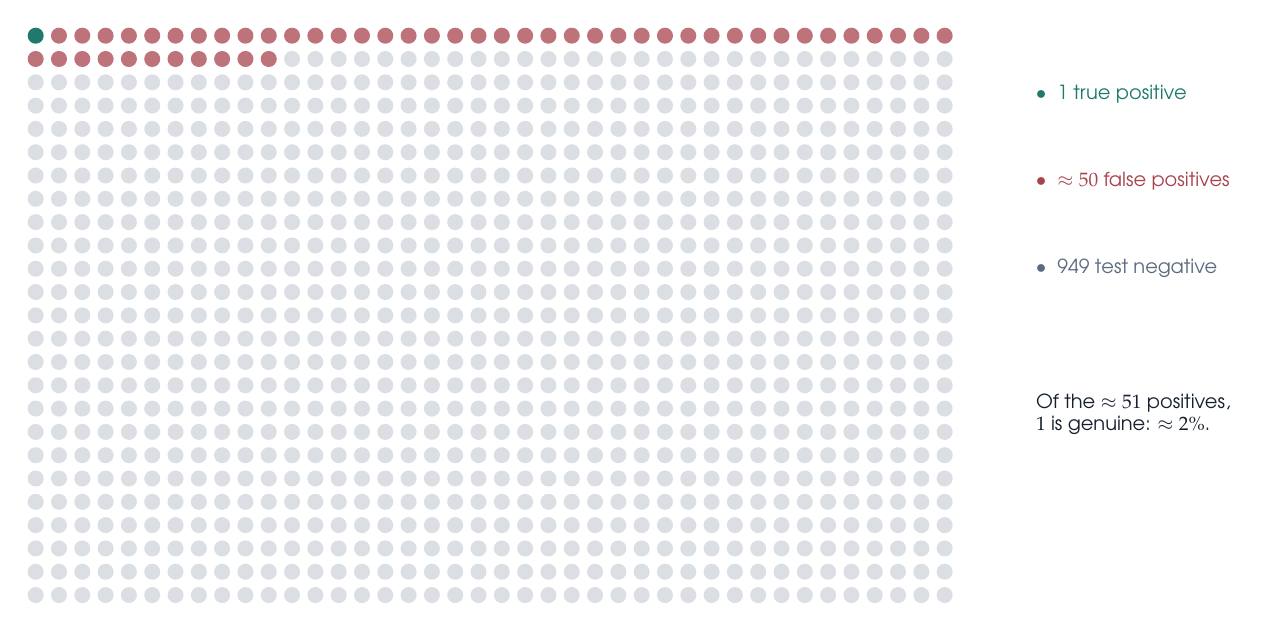
\begin{tikzpicture}[x=0.185cm,y=0.185cm]
  % 1000 dots: 1 true positive-ish, ~50 false positives
  \foreach \i in {0,...,999}{
    \pgfmathtruncatemacro{\row}{floor(\i/40)}
    \pgfmathtruncatemacro{\col}{mod(\i,40)}
    \ifnum\i=0
      \fill[teal] (\col*1.6,-\row*1.6) circle (0.55);
    \else
      \ifnum\i<51
        \fill[rose!75] (\col*1.6,-\row*1.6) circle (0.55);
      \else
        \fill[slate!22] (\col*1.6,-\row*1.6) circle (0.55);
      \fi
    \fi
  }
  \node[font=\scriptsize\sffamily, color=teal, anchor=west] at (68,-4)
    {$\bullet$\; 1 true positive};
  \node[font=\scriptsize\sffamily, color=rose, anchor=west] at (68,-10)
    {$\bullet$\; $\approx 50$ false positives};
  \node[font=\scriptsize\sffamily, color=slate, anchor=west] at (68,-16)
    {$\bullet$\; 949 test negative};
  \node[font=\scriptsize\sffamily, color=ink, anchor=west, align=left] at (68,-26)
    {Of the $\approx 51$ positives,\\ $1$ is genuine: $\approx 2\%$.};
\end{tikzpicture}
\caption{Natural frequencies. Conditional probability becomes obvious the moment you
count objects instead of manipulating fractions: restrict to the coloured dots and ask
what fraction is green.}
\end{figure}

\begin{warnbox}[The two most common conditional-probability errors]
\begin{itemize}
  \item \keyw{Transposing the conditional.} $\Prob(A\given B) \neq \Prob(B\given A)$ in
        general. They are related by Bayes and differ by the ratio
        $\Prob(A)/\Prob(B)$.
  \item \keyw{Forgetting to condition on the information-generating process.} What you
        learn is not ``a fact'' but ``a fact was reported to me by some mechanism''.
        The two-child problem turns on exactly this: ``at least one is a boy'' gives
        $\Prob(\text{both boys}) = 1/3$, while ``the elder is a boy'' gives $1/2$, and
        ``I met one of them at random and he is a boy'' gives $1/2$. Same words,
        different sample spaces.
\end{itemize}
\end{warnbox}
% ---- end ch09-conditional.tex ----
% ---- begin ch10-expectation.tex ----
\section{Expectation, and the one trick that solves everything}
\label{sec:expectation}

\begin{defbox}[Random variable, PMF, expectation]
A \keyw{discrete random variable} is a function $X : S \to \R$ taking countably many
values. Its \keyw{probability mass function} is $p_X(x) = \Prob(X=x)$, and its
\keyw{expectation} (mean, expected value) is
\[
  \E[X] \;=\; \sum_{x} x\,\Prob(X=x),
\]
provided $\sum_x \lvert x\rvert \Prob(X=x) < \infty$. Interpretation: the long-run
average value of $X$ over many independent repetitions, and the centre of mass of the
PMF.
\end{defbox}

\begin{thmbox}[Linearity of expectation]
For \emph{any} random variables $X_1,\dots,X_n$ on the same sample space and any
constants $a_i, b$,
\[
  \E\!\left[\sum_{i=1}^{n} a_i X_i + b\right] \;=\; \sum_{i=1}^{n} a_i\,\E[X_i] + b .
\]
\keyw{No independence is required.} The $X_i$ may be wildly dependent; linearity still
holds, because it is just a rearrangement of a finite (or absolutely convergent) sum
over the sample space.
\end{thmbox}

\begin{ideabox}[The indicator method]
To find $\E[X]$ where $X$ counts how many things happen:
\begin{enumerate}
  \item Write $X = \one_{A_1} + \one_{A_2} + \dots + \one_{A_n}$, one indicator per
        thing that could happen.
  \item Note $\E[\one_{A}] = \Prob(A)$, since $\one_A$ is $1$ with probability
        $\Prob(A)$ and $0$ otherwise.
  \item Conclude $\E[X] = \sum_{i=1}^{n}\Prob(A_i)$.
\end{enumerate}
This converts a hard distributional question (what is the distribution of $X$?) into
$n$ easy questions (what is the chance of this one event?). It is by far the most
useful technique in elementary probability.
\end{ideabox}

\begin{exbox}[Four problems, one method]
\textbf{(a) Fixed points of a random permutation.} $X=\sum_{i=1}^{n}\one_{\{\sigma(i)=i\}}$,
and $\Prob(\sigma(i)=i)=1/n$, so $\E[X] = n\cdot\frac1n = 1$, for every $n$. The
distribution of $X$ is complicated (Section~\ref{sec:incexc}); its mean is not.

\medskip
\textbf{(b) Matching cards.} Two shuffled decks are dealt in parallel; the expected
number of positions where the cards agree is $52\cdot\frac{1}{52} = 1$.

\medskip
\textbf{(c) Ascents.} In a uniformly random permutation of $[n]$, the expected number of
$i$ with $\sigma(i)<\sigma(i+1)$ is $(n-1)\cdot\tfrac12 = \tfrac{n-1}{2}$, since each
adjacent pair is increasing with probability $1/2$.

\medskip
\textbf{(d) Records.} Reading a random permutation left to right, position $i$ is a
\emph{record} (larger than everything before it) with probability $1/i$, because the
maximum of the first $i$ entries is equally likely to be in any of the $i$ positions.
So the expected number of records is the harmonic number
\[
  H_n = \sum_{i=1}^{n}\frac1i \;\approx\; \ln n + \gamma, \qquad \gamma\approx 0.5772 .
\]
\end{exbox}

\begin{thmbox}[Other tools for computing $\E$]
\begin{center}
\begin{tabularx}{\textwidth}{@{}lX@{}}
\toprule
\keyw{LOTUS} & $\displaystyle \E[g(X)] = \sum_x g(x)\Prob(X=x)$: you do \emph{not} need the
   distribution of $g(X)$. \\
\keyw{Tail sum} & for $X$ taking values in $\{0,1,2,\dots\}$,
   $\displaystyle \E[X] = \sum_{k\ge 1}\Prob(X \ge k)$. \\
\keyw{Tower property} & $\E[X] = \E\bigl[\E[X\given Y]\bigr]$: condition on whatever makes
   the problem easy, then average. \\
\keyw{First-step analysis} & set up an equation for $\E[X]$ by conditioning on the first
   step, then solve algebraically. \\
\keyw{Symmetry} & if $X_1,\dots,X_n$ are exchangeable and sum to $T$, then
   $\E[X_i] = \E[T]/n$ without any further work. \\
\bottomrule
\end{tabularx}
\end{center}
\end{thmbox}

\begin{exbox}[First-step analysis: waiting for a run]
How many fair coin tosses on average until the first head? Let $\mu = \E[N]$. Condition
on the first toss: with probability $\tfrac12$ we are done in one toss; with probability
$\tfrac12$ we have used one toss and are back where we started. So
\[
  \mu = \tfrac12(1) + \tfrac12(1+\mu) \;\Longrightarrow\; \mu = 2 .
\]
For the first occurrence of \texttt{HH}, the same method with two states gives $6$; for
\texttt{HT} it gives $4$. \emph{Different patterns of the same length have different
waiting times}, which surprises almost everyone the first time. The reason is that
\texttt{HH} can overlap itself and \texttt{HT} cannot.
\end{exbox}

\begin{figure}[H]
\centering
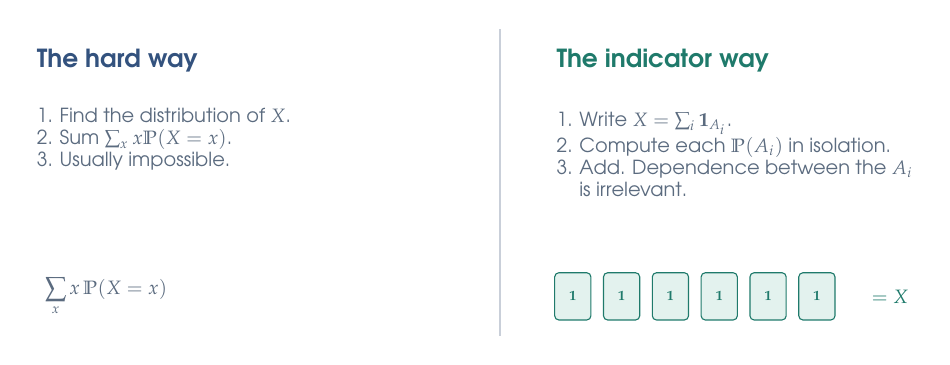
\begin{tikzpicture}[x=1cm,y=1cm]
  \node[font=\small\sffamily\bfseries, color=indigo, anchor=west] at (0,2.6) {The hard way};
  \node[font=\scriptsize\sffamily, color=slate, anchor=west, align=left] at (0,1.6)
    {1. Find the distribution of $X$.\\
     2. Sum $\sum_x x\Prob(X=x)$.\\
     3. Usually impossible.};
  \draw[rule, line width=0.7pt] (6.0,-0.9) -- (6.0,3.0);
  \node[font=\small\sffamily\bfseries, color=teal, anchor=west] at (6.6,2.6) {The indicator way};
  \node[font=\scriptsize\sffamily, color=slate, anchor=west, align=left] at (6.6,1.4)
    {1. Write $X=\sum_i \one_{A_i}$.\\
     2. Compute each $\Prob(A_i)$ in isolation.\\
     3. Add. Dependence between the $A_i$\\
     \hphantom{3. }is irrelevant.};
  \foreach \i in {0,...,5}{
    \pgfmathsetmacro{\xx}{6.7+\i*0.62}
    \draw[teal, fill=tealLt, rounded corners=1.5pt] (\xx,-0.7) rectangle (\xx+0.46,-0.1);
    \node[font=\tiny\sffamily, color=teal] at (\xx+0.23,-0.4) {$\one$};
  }
  \node[font=\scriptsize\sffamily, color=teal, anchor=west] at (10.6,-0.4) {$=X$};
  \node[font=\scriptsize\sffamily, color=slate, anchor=west] at (0.1,-0.4)
    {$\displaystyle\sum_x x\,\Prob(X=x)$};
\end{tikzpicture}
\caption{Linearity lets you decompose before you compute, which is the opposite of the
usual order of operations.}
\end{figure}

\begin{warnbox}[Linearity is for sums, not products]
$\E[XY] = \E[X]\E[Y]$ requires independence (or at least zero covariance).
$\E[X+Y]=\E[X]+\E[Y]$ requires nothing. Likewise $\E[g(X)] \neq g(\E[X])$ in general:
for convex $g$, Jensen's inequality gives $\E[g(X)] \ge g(\E[X])$. In particular
$\E[X^2] \ge (\E[X])^2$, with the gap being exactly the variance.
\end{warnbox}
% ---- end ch10-expectation.tex ----
% ---- begin ch11-variance.tex ----
\section{Variance, covariance, and how far from the mean}

\begin{defbox}[Variance and standard deviation]
\[
  \Var(X) \;\eqdef\; \E\bigl[(X-\E X)^2\bigr] \;=\; \E[X^2] - (\E X)^2,
  \qquad \SD(X) = \sqrt{\Var(X)} .
\]
The second form is the one you compute with. Variance is in squared units; the standard
deviation is in the same units as $X$, which is why it is the one that gets reported.
\end{defbox}

\begin{thmbox}[Rules]
\begin{align*}
  \Var(aX+b) &= a^{2}\Var(X) && \text{shifts do not change spread; scaling squares} \\
  \Cov(X,Y)  &= \E[XY]-\E[X]\E[Y] && \text{with } \Cov(X,X)=\Var(X) \\
  \Var\Bigl(\sum_i X_i\Bigr) &= \sum_i \Var(X_i) + 2\sum_{i<j}\Cov(X_i,X_j) & \\
  \Var\Bigl(\sum_i X_i\Bigr) &= \sum_i \Var(X_i) && \text{if the } X_i \text{ are pairwise uncorrelated} \\
  \Corr(X,Y) &= \frac{\Cov(X,Y)}{\SD(X)\,\SD(Y)} \in [-1,1] &
\end{align*}
\end{thmbox}

\begin{warnbox}[Variance is not linear]
The identity $\E[\sum X_i]=\sum \E[X_i]$ is unconditional. The analogous statement for
variance is \emph{false} without an assumption: dependent variables have a covariance
term. Independence implies zero covariance; the converse is false ($X$ uniform on
$\{-1,0,1\}$ and $Y=X^2$ have $\Cov=0$ but are utterly dependent).
\end{warnbox}

\begin{exbox}[Variance of a binomial, by indicators]
Let $X \sim \mathrm{Bin}(n,p)$, written as $X=\sum_{i=1}^{n}\one_{A_i}$ with
independent $A_i$ of probability $p$. For a single indicator,
\[
  \E[\one_{A}] = p, \qquad \E[\one_A^2] = \E[\one_A] = p,
  \qquad \Var(\one_A) = p - p^{2} = p(1-p).
\]
Independence kills the covariances, so $\Var(X) = np(1-p)$.

Now compare the \keyw{hypergeometric} case: drawing $n$ balls \emph{without}
replacement from $N$ balls of which $K$ are red. The indicators still each have mean
$p=K/N$, so $\E[X]=np$ exactly as before, by linearity. But now they are negatively
correlated (drawing a red one makes the next draw less likely to be red), and the
covariance term reduces the variance to
\[
  \Var(X) = np(1-p)\cdot\underbrace{\frac{N-n}{N-1}}_{\text{finite population correction}} .
\]
Same mean, smaller spread: sampling without replacement is more informative.
\end{exbox}

\subsection{How far from the mean can you get?}

\begin{thmbox}[Markov and Chebyshev]
For $X\ge 0$ and $a>0$: \quad
$\displaystyle \Prob(X \ge a) \le \frac{\E[X]}{a}$ \quad (Markov).

For any $X$ with finite variance and $k>0$: \quad
$\displaystyle \Prob\bigl(\lvert X-\E X\rvert \ge k\,\SD(X)\bigr) \le \frac{1}{k^{2}}$
\quad (Chebyshev).
\end{thmbox}

Chebyshev is Markov applied to $(X-\E X)^2$. Both are weak, and that weakness is the
point: they hold for \emph{every} distribution with the stated moments, so they are the
right tools when you know nothing else. When you do know more (independent bounded
summands, say), sharper exponential bounds are available.

\begin{figure}[H]
\centering
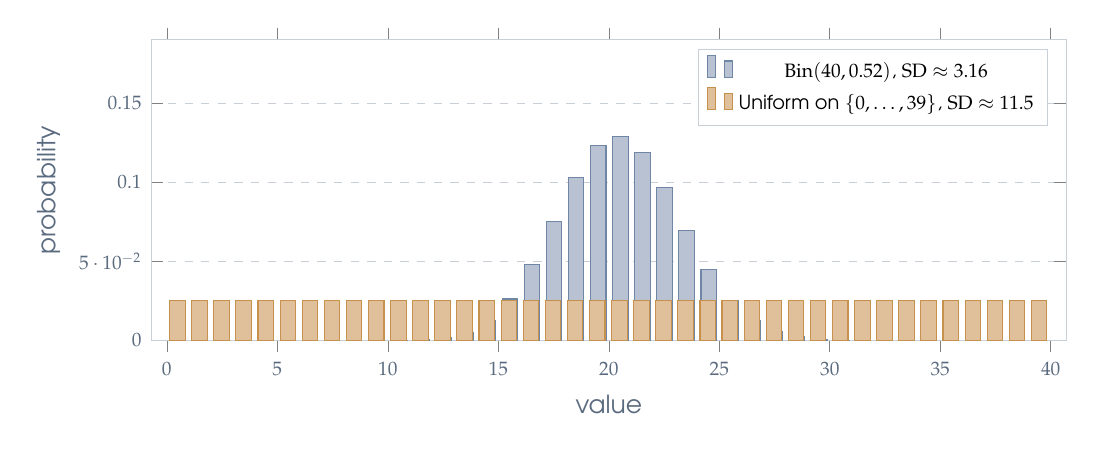
\begin{tikzpicture}
\begin{axis}[
  width=13.2cm, height=5.4cm,
  ybar, bar width=5.6pt,
  xlabel={value}, ylabel={probability},
  xlabel style={font=\small\sffamily, color=slate},
  ylabel style={font=\small\sffamily, color=slate},
  tick label style={font=\scriptsize\sffamily, color=slate},
  axis line style={color=rule},
  ymajorgrids, grid style={color=rule, dashed, line width=0.4pt},
  xmin=-0.7, xmax=40.7, ymin=0, ymax=0.19,
  xtick={0,5,10,15,20,25,30,35,40},
  legend style={font=\scriptsize\sffamily, draw=rule, fill=white, at={(0.98,0.97)}, anchor=north east},
]
\addplot[draw=indigo!70, fill=indigo!35] coordinates {
(10,0.0000)(11,0.0001)(12,0.0004)(13,0.0016)(14,0.0049)(15,0.0123)(16,0.0262)
(17,0.0478)(18,0.0752)(19,0.1029)(20,0.1229)(21,0.1289)(22,0.1189)(23,0.0968)
(24,0.0697)(25,0.0446)(26,0.0253)(27,0.0128)(28,0.0057)(29,0.0023)(30,0.0008)(31,0.0002)};
\addlegendentry{$\mathrm{Bin}(40,0.52)$, $\SD\approx 3.16$}
\addplot[draw=amber!80, fill=amber!45] coordinates {
(0,0.0250)(1,0.0250)(2,0.0250)(3,0.0250)(4,0.0250)(5,0.0250)(6,0.0250)(7,0.0250)
(8,0.0250)(9,0.0250)(10,0.0250)(11,0.0250)(12,0.0250)(13,0.0250)(14,0.0250)(15,0.0250)
(16,0.0250)(17,0.0250)(18,0.0250)(19,0.0250)(20,0.0250)(21,0.0250)(22,0.0250)(23,0.0250)
(24,0.0250)(25,0.0250)(26,0.0250)(27,0.0250)(28,0.0250)(29,0.0250)(30,0.0250)(31,0.0250)
(32,0.0250)(33,0.0250)(34,0.0250)(35,0.0250)(36,0.0250)(37,0.0250)(38,0.0250)(39,0.0250)};
\addlegendentry{Uniform on $\{0,\dots,39\}$, $\SD\approx 11.5$}
\end{axis}
\end{tikzpicture}
\caption{Two distributions with almost the same mean ($20.8$ and $19.5$) and completely
different variance. The mean tells you where; the variance tells you how much you
should trust it.}
\end{figure}

\begin{panel}[Moments in one place]
For a discrete $X$:
\[
  \E[X] = \sum_x x\,p(x), \qquad
  \E[X^2] = \sum_x x^2 p(x), \qquad
  \Var(X) = \E[X^2]-\E[X]^2 .
\]
The \keyw{probability generating function} $G_X(t) = \E[t^{X}] = \sum_k \Prob(X=k)t^k$
packages all of this: $G_X(1)=1$, $G_X'(1)=\E[X]$, $G_X''(1)=\E[X(X-1)]$, and hence
$\Var(X) = G_X''(1)+G_X'(1)-\bigl(G_X'(1)\bigr)^2$. For independent $X,Y$,
$G_{X+Y}=G_X G_Y$, which is why sums of independent binomials with the same $p$ are
binomial: $\bigl((1-p)+pt\bigr)^{m}\bigl((1-p)+pt\bigr)^{n} = \bigl((1-p)+pt\bigr)^{m+n}$.
\end{panel}
% ---- end ch11-variance.tex ----
% ---- begin ch12-distributions.tex ----
\section{The named discrete distributions}
\label{sec:dists}

Six distributions cover almost everything. They are not six unrelated facts: they are
six different questions asked about the same repeated experiment.

\begin{figure}[H]
\centering
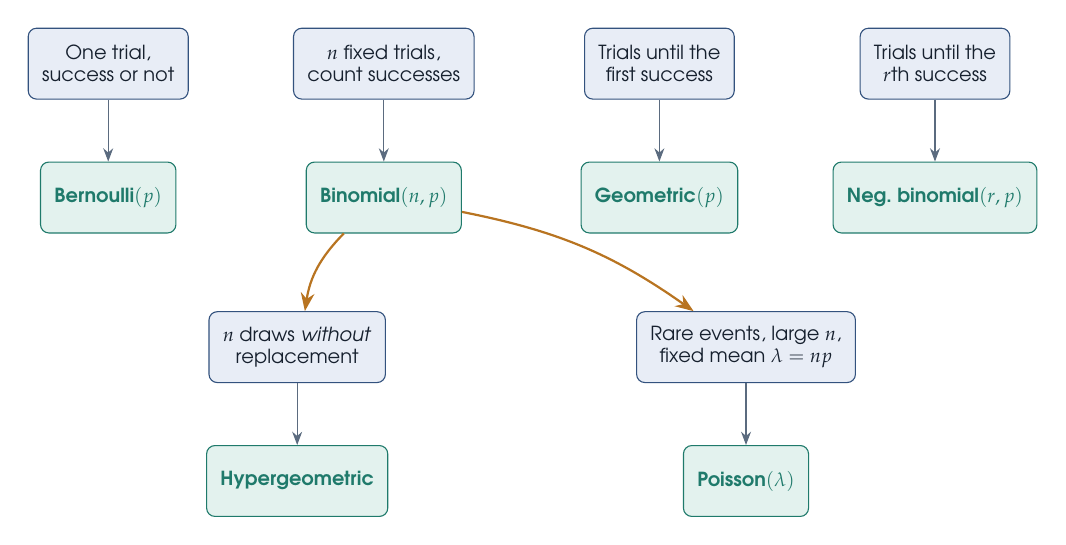
\begin{tikzpicture}[
  node distance=8mm,
  q/.style={rectangle, rounded corners=3pt, draw=indigo, fill=indigoLt, inner sep=5pt,
            font=\scriptsize\sffamily, text=ink, align=center, minimum height=9mm},
  d/.style={rectangle, rounded corners=3pt, draw=teal, fill=tealLt, inner sep=5pt,
            font=\scriptsize\sffamily\bfseries, text=teal, align=center, minimum height=9mm},
  >=Stealth
]
\node[q] (a) at (0,0) {One trial,\\ success or not};
\node[d] (ad) at (0,-1.7) {Bernoulli$(p)$};
\node[q] (b) at (3.5,0) {$n$ fixed trials,\\ count successes};
\node[d] (bd) at (3.5,-1.7) {Binomial$(n,p)$};
\node[q] (c) at (7.0,0) {Trials until the\\ first success};
\node[d] (cd) at (7.0,-1.7) {Geometric$(p)$};
\node[q] (d) at (10.5,0) {Trials until the\\ $r$th success};
\node[d] (dd) at (10.5,-1.7) {Neg.\ binomial$(r,p)$};
\node[q] (e) at (2.4,-3.6) {$n$ draws \emph{without}\\ replacement};
\node[d] (ed) at (2.4,-5.3) {Hypergeometric};
\node[q] (f) at (8.1,-3.6) {Rare events, large $n$,\\ fixed mean $\lambda=np$};
\node[d] (fd) at (8.1,-5.3) {Poisson$(\lambda)$};
\foreach \x/\y in {a/ad,b/bd,c/cd,d/dd,e/ed,f/fd}{\draw[->, slate] (\x) -- (\y);}
\draw[->, amber, thick] (bd) to[bend right=18] (e);
\draw[->, amber, thick] (bd) to[bend left=12] (f);
\end{tikzpicture}
\caption{Which distribution is which question.}
\end{figure}

\subsection{The reference table}

\begin{table}[H]
\centering
{\footnotesize
\setlength{\tabcolsep}{5pt}
\renewcommand{\arraystretch}{1.75}
\begin{tabular}{@{}l l l c c@{}}
\toprule
\sffamily\bfseries\color{slate}Distribution &
\sffamily\bfseries\color{slate}Support &
\sffamily\bfseries\color{slate}PMF $\Prob(X=k)$ &
\sffamily\bfseries\color{slate}Mean &
\sffamily\bfseries\color{slate}Variance \\
\midrule
\textcolor{indigo}{\bfseries Bernoulli$(p)$} & $\{0,1\}$ & $p^{k}(1-p)^{1-k}$ & $p$ & $p(1-p)$ \\
\textcolor{indigo}{\bfseries Binomial$(n,p)$} & $0,1,\dots,n$ & $\comb{n}{k}\,p^{k}(1-p)^{n-k}$ & $np$ & $np(1-p)$ \\
\textcolor{indigo}{\bfseries Geometric$(p)$} & $1,2,3,\dots$ & $(1-p)^{k-1}p$ & $\dfrac1p$ & $\dfrac{1-p}{p^{2}}$ \\
\textcolor{indigo}{\bfseries Neg.\ binomial$(r,p)$} & $r,r+1,\dots$ & $\comb{k-1}{r-1}p^{r}(1-p)^{k-r}$ & $\dfrac{r}{p}$ & $\dfrac{r(1-p)}{p^{2}}$ \\
\textcolor{indigo}{\bfseries Hypergeom.$(N,K,n)$} & {\scriptsize$\max(0,n{-}N{+}K)\dots\min(n,K)$} &
  $\dfrac{\comb{K}{k}\comb{N-K}{n-k}}{\comb{N}{n}}$ & $n\pi$ &
  $n\pi(1-\pi)\dfrac{N-n}{N-1}$ \\
\textcolor{indigo}{\bfseries Poisson$(\lambda)$} & $0,1,2,\dots$ & $e^{-\lambda}\dfrac{\lambda^{k}}{k!}$ & $\lambda$ & $\lambda$ \\
\textcolor{indigo}{\bfseries Uniform on $[n]$} & $1,2,\dots,n$ & $\dfrac1n$ & $\dfrac{n+1}{2}$ & $\dfrac{n^{2}-1}{12}$ \\
\bottomrule
\end{tabular}}

{\footnotesize\color{slate}For the hypergeometric, $\pi = K/N$ is the proportion of
successes in the population.}
\caption{Every PMF here sums to $1$ by an identity from Part~I: binomial by the binomial
theorem, negative binomial by Newton's series, hypergeometric by Vandermonde, Poisson by
the exponential series.}
\end{table}

\begin{ideabox}[Read the table as counting]
$\comb{n}{k}p^{k}(1-p)^{n-k}$: choose \emph{which} $k$ of the $n$ trials succeed
($\comb{n}{k}$), then the probability of that specific pattern ($p^k(1-p)^{n-k}$, by
independence). The binomial coefficient is doing exactly the job it did in Part I.

$\comb{k-1}{r-1}p^{r}(1-p)^{k-r}$: the $k$th trial must be the $r$th success, so choose
which $r-1$ of the first $k-1$ trials were the earlier successes.

$\comb{K}{k}\comb{N-K}{n-k}\big/\comb{N}{n}$: this is the equally-likely model,
$\lvert A\rvert/\lvert S\rvert$, with $\lvert S\rvert = \comb{N}{n}$ subsets of size $n$.
\end{ideabox}

\subsection{How the shape depends on the parameters}

\begin{figure}[H]
\centering
% ---- begin fig-binshape.tex ----
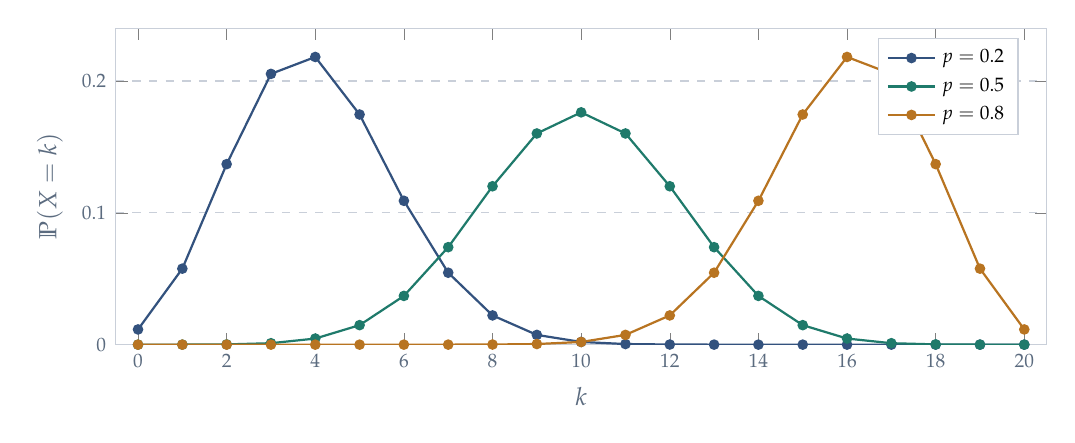
\begin{tikzpicture}
\begin{axis}[
  width=13.4cm, height=5.6cm,
  xlabel style={font=\small\sffamily, color=slate},
  ylabel style={font=\small\sffamily, color=slate},
  tick label style={font=\scriptsize\sffamily, color=slate},
  axis line style={color=rule},
  ymajorgrids, grid style={color=rule, dashed, line width=0.4pt},
  legend style={font=\scriptsize\sffamily, draw=rule, fill=white},
  legend cell align=left,
  xlabel={$k$}, ylabel={$\Prob(X=k)$}, xmin=-0.5, xmax=20.5, ymin=0, ymax=0.24,
  xtick={0,2,4,6,8,10,12,14,16,18,20}, legend pos=north east,
]
\addplot[color=indigo, mark=*, mark size=1.5pt, thick] coordinates {(0,0.011529) (1,0.057646) (2,0.136909) (3,0.205364) (4,0.218199) (5,0.174560) (6,0.109100) (7,0.054550) (8,0.022161) (9,0.007387) (10,0.002031) (11,0.000462) (12,0.000087) (13,0.000013) (14,0.000002) (15,0.000000) (16,0.000000) (17,0.000000) (18,0.000000) (19,0.000000) (20,0.000000)};
\addlegendentry{$p=0.2$}
\addplot[color=teal, mark=*, mark size=1.5pt, thick] coordinates {(0,0.000001) (1,0.000019) (2,0.000181) (3,0.001087) (4,0.004621) (5,0.014786) (6,0.036964) (7,0.073929) (8,0.120134) (9,0.160179) (10,0.176197) (11,0.160179) (12,0.120134) (13,0.073929) (14,0.036964) (15,0.014786) (16,0.004621) (17,0.001087) (18,0.000181) (19,0.000019) (20,0.000001)};
\addlegendentry{$p=0.5$}
\addplot[color=amber, mark=*, mark size=1.5pt, thick] coordinates {(0,0.000000) (1,0.000000) (2,0.000000) (3,0.000000) (4,0.000000) (5,0.000000) (6,0.000002) (7,0.000013) (8,0.000087) (9,0.000462) (10,0.002031) (11,0.007387) (12,0.022161) (13,0.054550) (14,0.109100) (15,0.174560) (16,0.218199) (17,0.205364) (18,0.136909) (19,0.057646) (20,0.011529)};
\addlegendentry{$p=0.8$}
\end{axis}
\end{tikzpicture}
% ---- end fig-binshape.tex ----
\caption{$\mathrm{Bin}(20,p)$. The mean sits at $np$; the distribution is symmetric only
at $p=\tfrac12$, right-skewed for small $p$, left-skewed for large $p$. Variance
$np(1-p)$ is largest at $p=\tfrac12$ and vanishes at the extremes.}
\end{figure}

\begin{figure}[H]
\centering
% ---- begin fig-hyper.tex ----
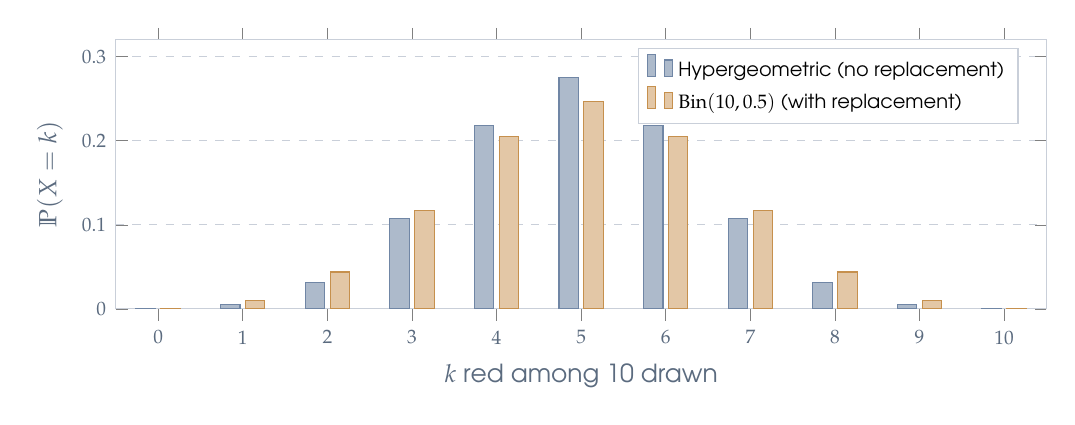
\begin{tikzpicture}
\begin{axis}[
  width=13.4cm, height=5.0cm,
  xlabel style={font=\small\sffamily, color=slate},
  ylabel style={font=\small\sffamily, color=slate},
  tick label style={font=\scriptsize\sffamily, color=slate},
  axis line style={color=rule},
  ymajorgrids, grid style={color=rule, dashed, line width=0.4pt},
  legend style={font=\scriptsize\sffamily, draw=rule, fill=white},
  legend cell align=left,
  xlabel={$k$ red among 10 drawn}, ylabel={$\Prob(X=k)$}, xmin=-0.5, xmax=10.5, ymin=0, ymax=0.32,
  xtick={0,1,2,3,4,5,6,7,8,9,10}, ybar, bar width=7pt, legend pos=north east,
]
\addplot[draw=indigo!70, fill=indigo!40] coordinates {(0,0.000318) (1,0.004972) (2,0.031587) (3,0.107630) (4,0.218093) (5,0.274798) (6,0.218093) (7,0.107630) (8,0.031587) (9,0.004972) (10,0.000318)};
\addlegendentry{Hypergeometric (no replacement)}
\addplot[draw=amber!80, fill=amber!40] coordinates {(0,0.000977) (1,0.009766) (2,0.043945) (3,0.117188) (4,0.205078) (5,0.246094) (6,0.205078) (7,0.117188) (8,0.043945) (9,0.009766) (10,0.000977)};
\addlegendentry{$\mathrm{Bin}(10,0.5)$ (with replacement)}
\end{axis}
\end{tikzpicture}
% ---- end fig-hyper.tex ----
\caption{Hypergeometric versus binomial with the same mean. Sampling without replacement
is more concentrated: the finite-population correction $\frac{N-n}{N-1}$ is less than
$1$ whenever $n>1$. As $N\to\infty$ with $K/N$ fixed, the two coincide.}
\end{figure}

\subsection{The Poisson limit}

\begin{thmbox}[Poisson limit theorem]
If $n\to\infty$ and $p\to 0$ with $np \to \lambda$ fixed, then for each $k$
\[
  \comb{n}{k}p^{k}(1-p)^{n-k} \;\longrightarrow\; e^{-\lambda}\frac{\lambda^{k}}{k!} .
\]
\textbf{Sketch.} With $p=\lambda/n$,
\[
  \comb{n}{k}p^k(1-p)^{n-k}
  = \underbrace{\frac{\ffact{n}{k}}{n^{k}}}_{\to\,1}\cdot\frac{\lambda^{k}}{k!}\cdot
    \underbrace{\Bigl(1-\frac{\lambda}{n}\Bigr)^{n}}_{\to\,e^{-\lambda}}\cdot
    \underbrace{\Bigl(1-\frac{\lambda}{n}\Bigr)^{-k}}_{\to\,1}.
\]
The falling factorial from Section~2 is what makes the first factor tend to $1$.
\end{thmbox}

\begin{figure}[H]
\centering
% ---- begin fig-poisson.tex ----
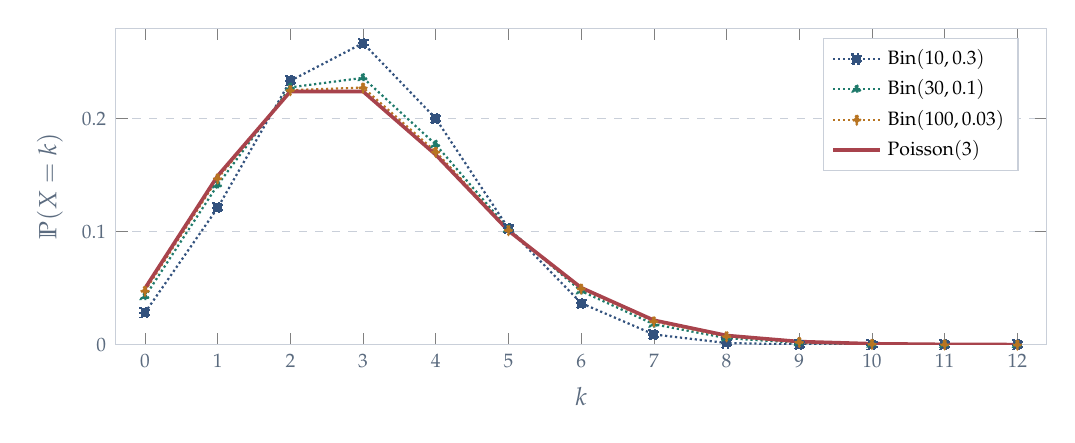
\begin{tikzpicture}
\begin{axis}[
  width=13.4cm, height=5.6cm,
  xlabel style={font=\small\sffamily, color=slate},
  ylabel style={font=\small\sffamily, color=slate},
  tick label style={font=\scriptsize\sffamily, color=slate},
  axis line style={color=rule},
  ymajorgrids, grid style={color=rule, dashed, line width=0.4pt},
  legend style={font=\scriptsize\sffamily, draw=rule, fill=white},
  legend cell align=left,
  xlabel={$k$}, ylabel={$\Prob(X=k)$}, xmin=-0.4, xmax=12.4, ymin=0, ymax=0.28,
  xtick={0,1,2,3,4,5,6,7,8,9,10,11,12}, legend pos=north east,
]
\addplot[color=indigo, mark=square*, mark size=1.6pt, thick, densely dotted] coordinates {(0,0.028248) (1,0.121061) (2,0.233474) (3,0.266828) (4,0.200121) (5,0.102919) (6,0.036757) (7,0.009002) (8,0.001447) (9,0.000138) (10,0.000006) (11,0.000000) (12,0.000000)};
\addlegendentry{$\mathrm{Bin}(10,0.3)$}
\addplot[color=teal, mark=triangle*, mark size=1.6pt, thick, densely dotted] coordinates {(0,0.042391) (1,0.141304) (2,0.227656) (3,0.236088) (4,0.177066) (5,0.102305) (6,0.047363) (7,0.018043) (8,0.005764) (9,0.001565) (10,0.000365) (11,0.000074) (12,0.000013)};
\addlegendentry{$\mathrm{Bin}(30,0.1)$}
\addplot[color=amber, mark=diamond*, mark size=1.6pt, thick, densely dotted] coordinates {(0,0.047553) (1,0.147070) (2,0.225153) (3,0.227474) (4,0.170606) (5,0.101308) (6,0.049610) (7,0.020604) (8,0.007408) (9,0.002342) (10,0.000659) (11,0.000167) (12,0.000038)};
\addlegendentry{$\mathrm{Bin}(100,0.03)$}
\addplot[color=rose, line width=1.3pt] coordinates {(0,0.049787) (1,0.149361) (2,0.224042) (3,0.224042) (4,0.168031) (5,0.100819) (6,0.050409) (7,0.021604) (8,0.008102) (9,0.002701) (10,0.000810) (11,0.000221) (12,0.000055)};
\addlegendentry{$\mathrm{Poisson}(3)$}
\end{axis}
\end{tikzpicture}
% ---- end fig-poisson.tex ----
\caption{Three binomials with mean $3$ converging on $\mathrm{Poisson}(3)$. By $n=100$,
$p=0.03$ the two are indistinguishable at this scale. Rule of thumb: the approximation
is good when $n \ge 20$ and $p \le 0.05$, or $n\ge 100$ and $np \le 10$.}
\end{figure}

\begin{panel}[Poisson facts worth carrying]
\begin{itemize}
  \item Mean $=$ variance $=\lambda$. If your data has variance far from its mean, it is
        not Poisson.
  \item Sums: $X\sim\mathrm{Poisson}(\lambda)$, $Y\sim\mathrm{Poisson}(\mu)$ independent
        $\Rightarrow X+Y \sim \mathrm{Poisson}(\lambda+\mu)$.
  \item Thinning: keep each Poisson$(\lambda)$ event independently with probability $q$;
        the survivors are $\mathrm{Poisson}(\lambda q)$.
  \item $\Prob(X=0)=e^{-\lambda}$, which is the single most-used value.
\end{itemize}
\end{panel}

\subsection{The normal approximation}

\begin{thmbox}[de Moivre--Laplace]
For $X\sim\mathrm{Bin}(n,p)$ with $np(1-p)$ large,
\[
  \Prob(a \le X \le b) \;\approx\;
  \Phi\!\left(\frac{b+\tfrac12-np}{\sqrt{np(1-p)}}\right)
  - \Phi\!\left(\frac{a-\tfrac12-np}{\sqrt{np(1-p)}}\right),
\]
where $\Phi$ is the standard normal CDF. The $\pm\tfrac12$ is the \keyw{continuity
correction}: you are approximating a bar of width $1$ by an area under a curve.
Rule of thumb: usable when $np \ge 10$ and $n(1-p)\ge 10$.
\end{thmbox}

\begin{figure}[H]
\centering
% ---- begin fig-normal.tex ----
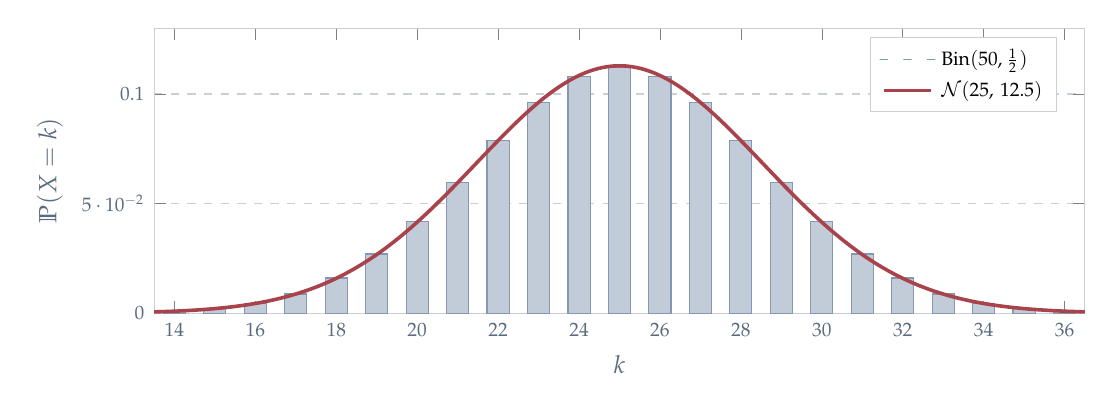
\begin{tikzpicture}
\begin{axis}[
  width=13.4cm, height=5.2cm,
  xlabel style={font=\small\sffamily, color=slate},
  ylabel style={font=\small\sffamily, color=slate},
  tick label style={font=\scriptsize\sffamily, color=slate},
  axis line style={color=rule},
  ymajorgrids, grid style={color=rule, dashed, line width=0.4pt},
  legend style={font=\scriptsize\sffamily, draw=rule, fill=white},
  legend cell align=left,
  xlabel={$k$}, ylabel={$\Prob(X=k)$}, xmin=13.5, xmax=36.5, ymin=0, ymax=0.13,
  xtick={14,16,18,20,22,24,26,28,30,32,34,36}, legend pos=north east,
]
\addplot[ybar, bar width=8pt, draw=indigo!60, fill=indigo!30] coordinates {(11,0.000033) (12,0.000108) (13,0.000315) (14,0.000833) (15,0.001999) (16,0.004373) (17,0.008746) (18,0.016035) (19,0.027006) (20,0.041859) (21,0.059799) (22,0.078826) (23,0.095962) (24,0.107957) (25,0.112275) (26,0.107957) (27,0.095962) (28,0.078826) (29,0.059799) (30,0.041859) (31,0.027006) (32,0.016035) (33,0.008746) (34,0.004373) (35,0.001999) (36,0.000833) (37,0.000315) (38,0.000108) (39,0.000033)};
\addlegendentry{$\mathrm{Bin}(50,\tfrac12)$}
\addplot[domain=13.5:36.5, samples=200, color=rose, line width=1.3pt]
  {1/(3.5355*sqrt(2*pi))*exp(-(x-25)^2/(2*12.5))};
\addlegendentry{$\mathcal{N}(25,\,12.5)$}
\end{axis}
\end{tikzpicture}
% ---- end fig-normal.tex ----
\caption{Row $50$ of Pascal's triangle, normalised, against the normal density with the
same mean and variance. The bell shape you noticed in Section~5 was the central limit
theorem all along.}
\end{figure}

\begin{exbox}[Which one is it?]
\begin{enumerate}[label=\textbf{\arabic*.}]
  \item \emph{Twelve fair dice are rolled; how many show a six?}
        Fixed number of independent trials, count successes: $\mathrm{Bin}(12,\tfrac16)$,
        mean $2$, variance $\tfrac{5}{3}$.
  \item \emph{How many rolls until the first six?}
        $\mathrm{Geometric}(\tfrac16)$, mean $6$, variance $30$.
  \item \emph{Five cards are dealt from a deck; how many are hearts?}
        No replacement: $\mathrm{Hypergeometric}(52,13,5)$, mean $5\cdot\tfrac{13}{52}=1.25$.
  \item \emph{A page has $2000$ characters, each mistyped with probability $0.001$;
        how many typos?} Rare, many trials: $\mathrm{Poisson}(2)$, so
        $\Prob(\text{no typos}) = e^{-2} \approx 0.135$.
\end{enumerate}
\end{exbox}
% ---- end ch12-distributions.tex ----
% ---- begin ch13-classics.tex ----
\section{Classic problems}

These are the problems that everyone meets, gets wrong, and then never forgets. Each one
isolates a single idea.

\subsection{The birthday problem}

\begin{exbox}[How many people before a shared birthday is likely?]
With $n$ people and $365$ equally likely birthdays, use the complement:
\[
  \Prob(\text{all distinct}) = \frac{\perm{365}{n}}{365^{n}}
  = \prod_{i=0}^{n-1}\left(1-\frac{i}{365}\right),
  \qquad
  \Prob(\text{some match}) = 1 - \frac{\perm{365}{n}}{365^{n}} .
\]
At $n=23$ this exceeds $\tfrac12$; at $n=57$ it exceeds $0.99$.
\end{exbox}

\begin{figure}[H]
\centering
% ---- begin fig-birthday.tex ----
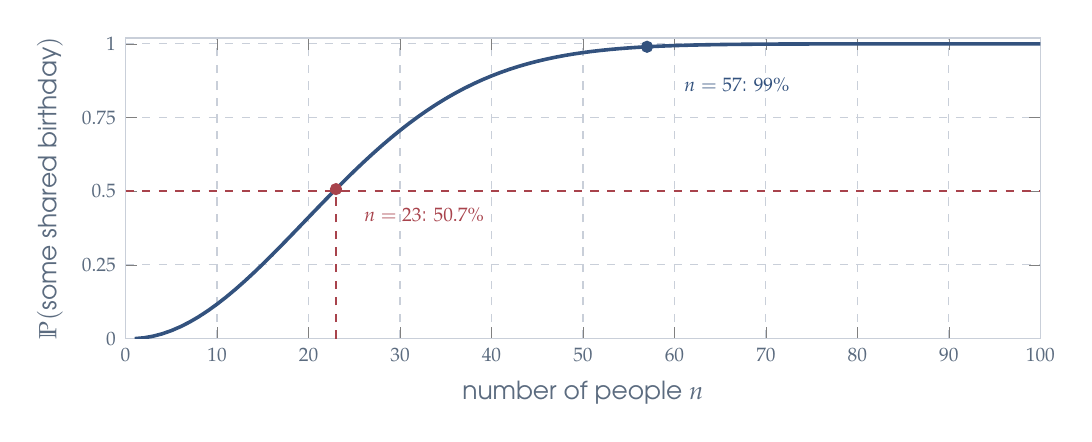
\begin{tikzpicture}
\begin{axis}[
  width=13.2cm, height=5.4cm,
  xlabel={number of people $n$}, ylabel={$\Prob(\text{some shared birthday})$},
  xlabel style={font=\small\sffamily, color=slate},
  ylabel style={font=\small\sffamily, color=slate},
  tick label style={font=\scriptsize\sffamily, color=slate},
  axis line style={color=rule}, ymajorgrids, xmajorgrids,
  grid style={color=rule, dashed, line width=0.4pt},
  xmin=0, xmax=100, ymin=0, ymax=1.02, xtick={0,10,...,100}, ytick={0,0.25,0.5,0.75,1},
]
\addplot[color=indigo, line width=1.3pt] coordinates {(1,0.000000) (2,0.002740) (3,0.008204) (4,0.016356) (5,0.027136) (6,0.040462) (7,0.056236) (8,0.074335) (9,0.094624) (10,0.116948) (11,0.141141) (12,0.167025) (13,0.194410) (14,0.223103) (15,0.252901) (16,0.283604) (17,0.315008) (18,0.346911) (19,0.379119) (20,0.411438) (21,0.443688) (22,0.475695) (23,0.507297) (24,0.538344) (25,0.568700) (26,0.598241) (27,0.626859) (28,0.654461) (29,0.680969) (30,0.706316) (31,0.730455) (32,0.753348) (33,0.774972) (34,0.795317) (35,0.814383) (36,0.832182) (37,0.848734) (38,0.864068) (39,0.878220) (40,0.891232) (41,0.903152) (42,0.914030) (43,0.923923) (44,0.932885) (45,0.940976) (46,0.948253) (47,0.954774) (48,0.960598) (49,0.965780) (50,0.970374) (51,0.974432) (52,0.978005) (53,0.981138) (54,0.983877) (55,0.986262) (56,0.988332) (57,0.990122) (58,0.991665) (59,0.992989) (60,0.994123) (61,0.995089) (62,0.995910) (63,0.996604) (64,0.997190) (65,0.997683) (66,0.998096) (67,0.998440) (68,0.998726) (69,0.998964) (70,0.999160) (71,0.999321) (72,0.999453) (73,0.999561) (74,0.999649) (75,0.999720) (76,0.999777) (77,0.999824) (78,0.999861) (79,0.999891) (80,0.999914) (81,0.999933) (82,0.999948) (83,0.999960) (84,0.999969) (85,0.999976) (86,0.999982) (87,0.999986) (88,0.999989) (89,0.999992) (90,0.999994) (91,0.999995) (92,0.999997) (93,0.999997) (94,0.999998) (95,0.999999) (96,0.999999) (97,0.999999) (98,0.999999) (99,1.000000) (100,1.000000)};
\addplot[color=rose, dashed, line width=0.9pt] coordinates {(0,0.5) (100,0.5)};
\addplot[color=rose, dashed, line width=0.9pt] coordinates {(23,0) (23,0.5073)};
\node[font=\scriptsize\sffamily, color=rose, anchor=west] at (axis cs:25,0.42) {$n=23$: $50.7\%$};
\addplot[only marks, mark=*, mark size=2pt, color=rose] coordinates {(23,0.5073)};
\node[font=\scriptsize\sffamily, color=indigo, anchor=west] at (axis cs:60,0.86) {$n=57$: $99\%$};
\addplot[only marks, mark=*, mark size=2pt, color=indigo] coordinates {(57,0.9901)};
\end{axis}
\end{tikzpicture}
% ---- end fig-birthday.tex ----
\caption{The birthday curve. It rises far faster than intuition suggests.}
\end{figure}

\begin{ideabox}[Why $23$ and not $183$]
Intuition counts \emph{people}; the problem counts \emph{pairs}. With $n$ people there
are $\comb{n}{2}$ pairs, each matching with probability $1/365$, so the expected number
of matching pairs is $\comb{n}{2}/365$. This reaches $1$ at $\comb{n}{2}\approx 365$,
that is $n \approx 27$. Since matches are roughly Poisson,
$\Prob(\text{at least one}) \approx 1-\exp\bigl(-\comb{n}{2}/365\bigr)$, which crosses
$\tfrac12$ at $\comb{n}{2}\approx 365\ln 2 \approx 253$, giving $n\approx 23$.
\emph{Quadratic growth in $n$ is the whole phenomenon.} The same computation is why hash
collisions appear after about $\sqrt{N}$ insertions into $N$ buckets.
\end{ideabox}

\subsection{The coupon collector}

\begin{exbox}[How long to collect all $n$ coupons?]
Once you hold $i$ distinct coupons, each new one is new with probability $(n-i)/n$, so
the wait for the next new coupon is $\mathrm{Geometric}\bigl(\frac{n-i}{n}\bigr)$ with
mean $\frac{n}{n-i}$. The total time $T$ is the sum of these waits, and linearity gives
\[
  \E[T] = \sum_{i=0}^{n-1}\frac{n}{n-i} = n\sum_{j=1}^{n}\frac{1}{j} = n H_n
  \approx n\ln n + \gamma n + \tfrac12 .
\]
The waits are independent, so the variances add too:
$\Var(T) = \sum_{i=0}^{n-1}\frac{n\,i}{(n-i)^2} < \frac{\pi^2 n^2}{6}$.

For $n=50$: $\E[T] = 50\,H_{50} \approx 224.96$, so about $225$ purchases for $50$
coupons. Doubling $n$ slightly more than doubles the wait; the $\ln n$ factor is gentle.
\end{exbox}

\subsection{Monty Hall}

\begin{exbox}[Switch]
Three doors, one prize. You pick a door; the host, who knows where the prize is and who
\emph{always} opens a different door revealing no prize, does so. Should you switch?

Condition on where the prize is. Your initial pick is correct with probability
$\tfrac13$. Switching wins exactly when your initial pick was \emph{wrong}, which has
probability $\tfrac23$. So switching wins with probability $\tfrac23$, and staying with
probability $\tfrac13$.
\end{exbox}

\begin{figure}[H]
\centering
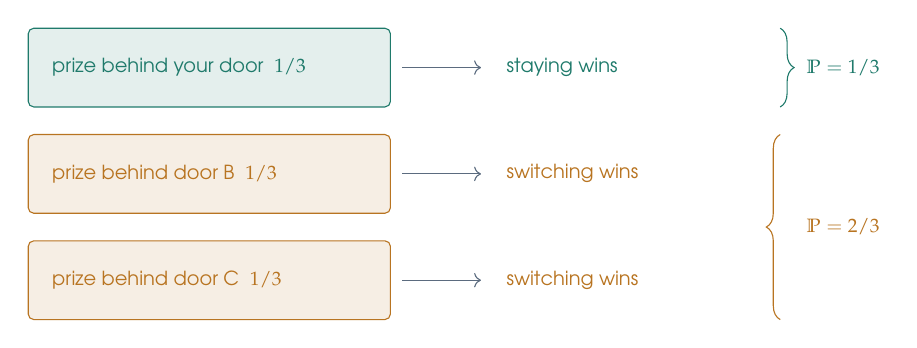
\begin{tikzpicture}[x=1cm,y=1cm]
  \foreach \i/\lab/\col/\p in {0/{prize behind your door}/teal/{$1/3$},
                               1/{prize behind door B}/amber/{$1/3$},
                               2/{prize behind door C}/amber/{$1/3$}}{
    \draw[draw=\col, fill=\col!12, rounded corners=2pt] (0,-\i*1.35) rectangle (4.6,-\i*1.35+1.0);
    \node[font=\scriptsize\sffamily, color=\col, anchor=west] at (0.18,-\i*1.35+0.5) {\lab\ \ \p};
    \draw[->, slate] (4.75,-\i*1.35+0.5) -- (5.75,-\i*1.35+0.5);
  }
  \node[font=\scriptsize\sffamily, color=teal, anchor=west] at (5.95,0.5)
    {staying wins};
  \node[font=\scriptsize\sffamily, color=amber, anchor=west] at (5.95,-0.85)
    {switching wins};
  \node[font=\scriptsize\sffamily, color=amber, anchor=west] at (5.95,-2.20)
    {switching wins};
  \draw[decorate, decoration={brace, amplitude=5pt}, amber]
    (9.55,-2.70) -- (9.55,-0.35) node[midway, right=6pt, font=\scriptsize\sffamily, color=amber] {$\Prob = 2/3$};
  \draw[decorate, decoration={brace, amplitude=5pt}, teal]
    (9.55,1.0) -- (9.55,0.0) node[midway, right=6pt, font=\scriptsize\sffamily, color=teal] {$\Prob = 1/3$};
\end{tikzpicture}
\caption{The host's action gives you no information about your own door, because he
would have opened \emph{some} empty door whatever you chose. All the information lands
on the remaining door.}
\end{figure}

\begin{warnbox}[The protocol is the problem]
Change the host's rule and the answer changes. If the host opens a door \emph{at
random} and it happens to be empty, switching wins with probability $\tfrac12$. The
words spoken are almost identical; the sample spaces are not. Whenever a problem
involves someone revealing information, write down explicitly what they would have done
in every case.
\end{warnbox}

\subsection{Two more worth knowing}

\begin{panel}[Quick classics]
\keyw{The matching / hat-check problem.} Expected matches $=1$; probability of no match
$\to e^{-1}$; number of matches is asymptotically $\mathrm{Poisson}(1)$
(Section~\ref{sec:incexc}).

\medskip
\keyw{The secretary problem.} To maximise the chance of selecting the best of $n$
candidates interviewed in random order, reject the first $\approx n/e$ and then take the
first candidate better than all seen so far. Success probability $\to 1/e \approx 0.368$,
independent of $n$.

\medskip
\keyw{Banach's matchbox.} Two boxes of $n$ matches, one drawn at random each time; when
one box is first found empty, the expected number remaining in the other is
$(2n+1)\dfrac{\comb{2n}{n}}{4^{n}} - 1 \approx 2\sqrt{n/\pi}$. The central binomial
coefficient from Section~5 appears again, and again with $\sqrt{\pi}$ in tow.
\end{panel}
% ---- end ch13-classics.tex ----
\clearpage
\part{Reference \& Practice}
% ---- begin ch14-reference.tex ----
\section{The one-page decision guide}

\begin{figure}[H]
\centering
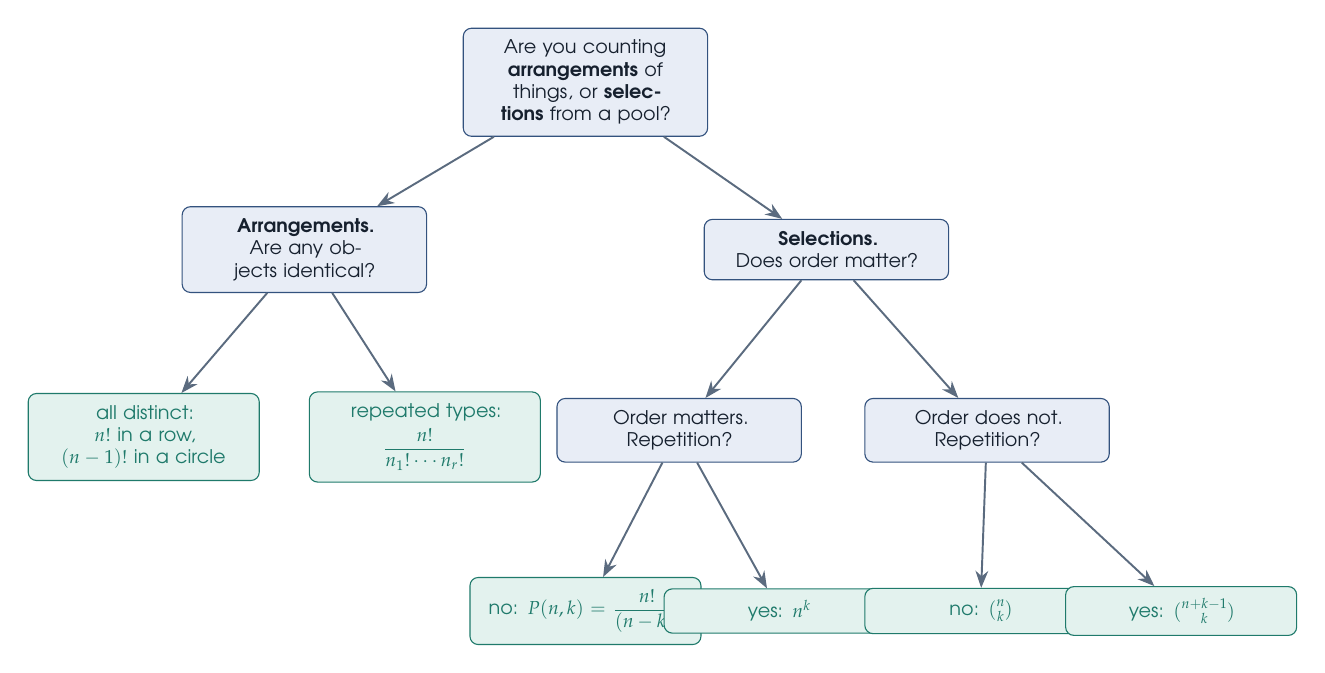
\begin{tikzpicture}[
  scale=0.85, transform shape,
  node distance=6mm,
  q/.style={rectangle, rounded corners=3pt, draw=indigo, fill=indigoLt, inner sep=5pt,
            font=\footnotesize\sffamily, text=ink, align=center, text width=3.3cm},
  a/.style={rectangle, rounded corners=3pt, draw=teal, fill=tealLt, inner sep=5pt,
            font=\footnotesize\sffamily, text=teal, align=center, text width=3.1cm},
  lab/.style={font=\scriptsize\sffamily, color=slate, fill=white, inner sep=1.5pt},
  >=Stealth, arr/.style={->, slate, line width=0.7pt}
]
\node[q] (start) at (0,0) {Are you counting \textbf{arrangements} of things, or
   \textbf{selections} from a pool?};

\node[q] (arr) at (-4.2,-2.5) {\textbf{Arrangements.}\\ Are any objects identical?};
\node[a] (arr1) at (-6.6,-5.3) {all distinct:\\ $n!$ in a row,\\ $(n-1)!$ in a circle};
\node[a] (arr2) at (-2.4,-5.3) {repeated types:\\[2pt]
   $\dfrac{n!}{n_1!\cdots n_r!}$};

\node[q] (sel) at (3.6,-2.5) {\textbf{Selections.}\\ Does order matter?};
\node[q] (selo) at (1.4,-5.2) {Order matters.\\ Repetition?};
\node[q] (selu) at (6.0,-5.2) {Order does not.\\ Repetition?};
\node[a] (s1) at (0.0,-7.9) {no: $\perm{n}{k}=\dfrac{n!}{(n-k)!}$};
\node[a] (s2) at (2.9,-7.9) {yes: $n^{k}$};
\node[a] (s3) at (5.9,-7.9) {no: $\comb{n}{k}$};
\node[a] (s4) at (8.9,-7.9) {yes: $\comb{n+k-1}{k}$};

\draw[arr] (start) -- (arr);
\draw[arr] (start) -- (sel);
\draw[arr] (arr) -- (arr1);
\draw[arr] (arr) -- (arr2);
\draw[arr] (sel) -- (selo);
\draw[arr] (sel) -- (selu);
\draw[arr] (selo) -- (s1);
\draw[arr] (selo) -- (s2);
\draw[arr] (selu) -- (s3);
\draw[arr] (selu) -- (s4);
\end{tikzpicture}
\caption{Four questions, four formulas. If none of the leaves fits, the object is
probably a \emph{partition} rather than a selection: see the panel in Section~6.}
\end{figure}

\begin{panel}[Signal words]
\begin{tabularx}{\textwidth}{@{}lX@{}}
\toprule
\emph{and}, ``then'', stages & multiply (product rule) \\
\emph{or}, ``either'', disjoint cases & add (sum rule) \\
\emph{at least one}, \emph{none} & take the complement, or inclusion--exclusion \\
\emph{at most}, upper bounds on variables & inclusion--exclusion \\
\emph{arrangement}, \emph{sequence}, \emph{ranking}, \emph{password} & order matters \\
\emph{committee}, \emph{subset}, \emph{hand}, \emph{team} & order does not matter \\
\emph{identical}, \emph{indistinguishable} objects into boxes & stars and bars \\
\emph{how many on average}, \emph{expected} & indicators plus linearity \\
\emph{given that}, \emph{knowing that} & conditional probability, Bayes \\
\bottomrule
\end{tabularx}
\end{panel}

\clearpage
\section{Formula spread}

\begin{panel}[Small values worth recognising]
{\footnotesize
\begin{tabularx}{\textwidth}{@{}lX@{}}
\toprule
$n!$ & $1,\ 1,\ 2,\ 6,\ 24,\ 120,\ 720,\ 5040,\ 40320,\ 362880,\ 3628800$ \\
$2^{n}$ & $1,\ 2,\ 4,\ 8,\ 16,\ 32,\ 64,\ 128,\ 256,\ 512,\ 1024,\ 2048,\ 4096$ \\
$\comb{2n}{n}$ & $1,\ 2,\ 6,\ 20,\ 70,\ 252,\ 924,\ 3432,\ 12870$ \\
Catalan $C_n$ & $1,\ 1,\ 2,\ 5,\ 14,\ 42,\ 132,\ 429,\ 1430,\ 4862$ \\
Derangements $D_n$ & $1,\ 0,\ 1,\ 2,\ 9,\ 44,\ 265,\ 1854,\ 14833$ \\
Bell $B_n$ & $1,\ 1,\ 2,\ 5,\ 15,\ 52,\ 203,\ 877,\ 4140$ \\
\bottomrule
\end{tabularx}}
\end{panel}

\vspace{6pt}

\setlength{\jot}{1pt}
\setlength{\abovedisplayskip}{3pt}\setlength{\belowdisplayskip}{3pt}
\setlength{\abovedisplayshortskip}{2pt}\setlength{\belowdisplayshortskip}{2pt}

\noindent
\begin{minipage}[t]{0.47\textwidth}
\subsection*{Counting}
\vspace{-8pt}
{\footnotesize
\begin{align*}
  n! &= n(n-1)\cdots 1, \quad 0!=1 \\
  \perm{n}{k} &= \frac{n!}{(n-k)!} = n(n-1)\cdots(n-k+1) \\
  \comb{n}{k} &= \frac{\perm{n}{k}}{k!} = \frac{n!}{k!(n-k)!} \\
  \binom{n}{n_1,\dots,n_r} &= \frac{n!}{n_1!\cdots n_r!} \\
  \text{strings} &: n^{k} \qquad \text{multisets}: \comb{n+k-1}{k} \\
  \text{circular} &: (n-1)! \qquad \text{necklace}: \tfrac{(n-1)!}{2}
\end{align*}}

\subsection*{Identities}
\vspace{-8pt}
{\footnotesize
\begin{align*}
  \comb{n}{k} &= \comb{n}{n-k} \\
  \comb{n}{k} &= \comb{n-1}{k-1}+\comb{n-1}{k} \\
  k\comb{n}{k} &= n\comb{n-1}{k-1} \\
  \sum_{k}\comb{n}{k} &= 2^{n}, \qquad \sum_k (-1)^k\comb{n}{k}=0 \\
  \sum_{k}k\comb{n}{k} &= n2^{n-1} \\
  \sum_{i=k}^{n}\comb{i}{k} &= \comb{n+1}{k+1} \\
  \sum_{j}\comb{m}{j}\comb{n}{k-j} &= \comb{m+n}{k} \\
  \sum_{k}\comb{n}{k}^{2} &= \comb{2n}{n}
\end{align*}}

\subsection*{Expansions}
\vspace{-8pt}
{\footnotesize
\begin{align*}
  (x+y)^{n} &= \sum_{k=0}^{n}\comb{n}{k}x^{n-k}y^{k} \\
  (1+t)^{\alpha} &= \sum_{k\ge0}\frac{\ffact{\alpha}{k}}{k!}t^{k}, \quad \lvert t\rvert<1 \\
  \frac{1}{(1-t)^{r}} &= \sum_{k\ge0}\comb{k+r-1}{r-1}t^{k} \\
  e^{x} &= \sum_{k\ge0}\frac{x^{k}}{k!}
\end{align*}}
\end{minipage}
\hfill
\begin{minipage}[t]{0.47\textwidth}
\subsection*{Probability}
\vspace{-8pt}
{\footnotesize
\begin{align*}
  \Prob(A) &= \frac{\lvert A\rvert}{\lvert S\rvert} \quad\text{(equally likely)} \\
  \Prob(\overline{A}) &= 1-\Prob(A) \\
  \Prob(A\cup B) &= \Prob(A)+\Prob(B)-\Prob(A\cap B) \\
  \Prob(A\given B) &= \frac{\Prob(A\cap B)}{\Prob(B)} \\
  \Prob(A) &= \sum_j \Prob(B_j)\Prob(A\given B_j) \\
  \Prob(B_i\given A) &= \frac{\Prob(B_i)\Prob(A\given B_i)}{\Prob(A)} \\
  \frac{\Prob(H_1\given E)}{\Prob(H_2\given E)}
    &= \frac{\Prob(H_1)}{\Prob(H_2)}\cdot\frac{\Prob(E\given H_1)}{\Prob(E\given H_2)}
\end{align*}}

\subsection*{Moments}
\vspace{-8pt}
{\footnotesize
\begin{align*}
  \E[X] &= \sum_x x\,\Prob(X=x) = \sum_{k\ge1}\Prob(X\ge k) \\
  \E\Bigl[\sum_i X_i\Bigr] &= \sum_i \E[X_i] \quad\text{(always)} \\
  \E[\one_A] &= \Prob(A) \\
  \Var(X) &= \E[X^{2}]-\E[X]^{2} \\
  \Var(aX+b) &= a^{2}\Var(X) \\
  \Var\Bigl(\sum_i X_i\Bigr) &= \sum_i\Var(X_i)+2\!\!\sum_{i<j}\!\Cov(X_i,X_j) \\
  \E[X] &= \E\bigl[\E[X\given Y]\bigr]
\end{align*}}

\subsection*{Approximations}
\vspace{-8pt}
{\footnotesize
\begin{align*}
  n! &\sim \sqrt{2\pi n}\left(\frac{n}{e}\right)^{n} \\
  \comb{2m}{m} &\sim \frac{4^{m}}{\sqrt{\pi m}} \\
  H_n &= \sum_{j=1}^{n}\tfrac1j \approx \ln n + \gamma, \ \gamma\approx0.5772 \\
  \Bigl(1-\tfrac{\lambda}{n}\Bigr)^{n} &\to e^{-\lambda} \\
  \mathrm{Bin}(n,p) &\approx \mathrm{Poisson}(np) \ \ (p \text{ small}) \\
  \mathrm{Bin}(n,p) &\approx \mathcal{N}\bigl(np,\,np(1-p)\bigr)
\end{align*}}
\end{minipage}

% ---- end ch14-reference.tex ----
% ---- begin ch15-problems.tex ----
\clearpage
\section{Problems}

Answers and full solutions follow in Section~\ref{sec:solutions}. Try them before
looking; the value is entirely in the attempt.

\begin{multicols}{2}
{\small
\subsection*{Counting}
\begin{enumerate}[label=\textbf{P\arabic*.}, leftmargin=2.4em]
\item How many five-letter words can be formed from the $26$ letters if no letter
      repeats?
\item How many distinguishable arrangements does \textsc{bookkeeper} have?
\item A committee of $5$ is chosen from $12$ people, and one member is designated chair.
      In how many ways? Give two derivations.
\item How many monotone lattice paths run from $(0,0)$ to $(7,5)$? How many of them pass
      through $(3,2)$?
\item How many solutions in integers does $a+b+c+d=20$ have with $0 \le a,b,c,d \le 9$?
\item Find the coefficient of $x^{5}$ in $(1+2x)^{9}$.
\item How many subsets of $\{1,\dots,10\}$ contain no two consecutive integers?
\item Eight people sit at a round table. In how many seatings are two particular people
      \emph{not} adjacent?
\item In how many permutations of $\{1,\dots,5\}$ does no element stay in its own place?
\item How many six-digit numbers (no leading zero) have digits summing to $10$?
\item In how many ways can $10$ identical balls go into $4$ distinct boxes with no box
      empty?
\item How many functions from a $5$-set onto a $3$-set are there?
\item Ten points lie in the plane with no three collinear. How many triangles do they
      determine?
\item Prove $\displaystyle\sum_{k=0}^{n}k^{2}\comb{n}{k} = n(n+1)2^{n-2}$.
\item How many binary strings of length $10$ have exactly three $1$s, no two adjacent?
\end{enumerate}

\subsection*{Probability}
\begin{enumerate}[label=\textbf{P\arabic*.}, leftmargin=2.4em, start=16]
\item Two fair dice are rolled. Given that at least one shows a $5$, what is the
      probability the total is $8$?
\item What is the probability that a five-card hand contains exactly two aces?
\item A fair die is rolled five times. What is the probability all five results differ?
\item One of two coins is chosen at random: one fair, one two-headed. It is flipped three
      times and lands heads every time. What is the probability it is the two-headed
      coin?
\item A fair die is rolled six times. What is the expected number of \emph{distinct}
      faces seen?
\item Show that the number of fixed points of a uniformly random permutation of $[n]$
      has variance $1$ for every $n \ge 2$.
\item On average, how many rolls of a fair die are needed to see all six faces?
\item A fair die is rolled ten times. What is the probability of at least two sixes?
\item Five people check hats and receive them back at random. What is the probability
      that exactly two people get their own hat?
\end{enumerate}}
\end{multicols}

\clearpage
\section{Solutions}
\label{sec:solutions}

{\small
\begin{enumerate}[label=\textbf{P\arabic*.}, leftmargin=2.6em, itemsep=6pt]

\item Ordered, no repetition:
      $\perm{26}{5} = 26\cdot25\cdot24\cdot23\cdot22 \ans{7\,893\,600}$.

\item \textsc{bookkeeper} has $10$ letters with \textsc{o} twice, \textsc{k} twice,
      \textsc{e} three times:
      $\dfrac{10!}{2!\,2!\,3!} = \dfrac{3\,628\,800}{24} \ans{151\,200}$.

\item \emph{Chair last:} $\comb{12}{5}\cdot 5 = 792\cdot 5 = 3960$.
      \emph{Chair first:} $12\cdot\comb{11}{4} = 12\cdot 330 = 3960$.
      The agreement is the absorption identity $k\comb{n}{k}=n\comb{n-1}{k-1}$
      with $n=12$, $k=5$. \ans{3960}

\item A path is a word with $7$ \texttt{R}s and $5$ \texttt{U}s:
      $\comb{12}{5} = 792$. Through $(3,2)$: split the path at that vertex,
      $\comb{5}{2}\comb{7}{3} = 10\cdot 35 \ans{350}$.

\item Without the upper bounds: $\comb{23}{3} = 1771$. Subtract, for each variable, the
      solutions where it is $\ge 10$ (shift by $10$, leaving total $10$):
      $4\comb{13}{3} = 4\cdot 286 = 1144$. Two variables can both exceed $9$ only if the
      total is at least $20$, which happens exactly when both equal $10$ and the others
      are $0$: add back $\comb{4}{2}\comb{3}{3} = 6$. Total
      $1771-1144+6 \ans{633}$.

\item $T_{k+1} = \comb{9}{k}(2x)^{k}$, so $k=5$ gives
      $\comb{9}{5}2^{5} = 126\cdot 32 \ans{4032}$.

\item Choose $m$ elements with no two adjacent from $[n]$: $\comb{n-m+1}{m}$ ways
      (a stars-and-bars argument on the gaps). Summing over $m=0,\dots,5$:
      $1+10+36+56+35+6 = 144 = F_{12}$, the Fibonacci number. \ans{144}

\item Total circular seatings $7! = 5040$. Seatings with the pair adjacent: glue them
      into a block, giving $6!$ circular arrangements of $7$ objects, times $2$ for the
      internal order: $2\cdot 720 = 1440$. Answer $5040-1440 \ans{3600}$.

\item $D_5 = 5!\bigl(1-1+\tfrac12-\tfrac16+\tfrac1{24}-\tfrac1{120}\bigr)
      = 120\cdot\tfrac{11}{30} \ans{44}$. (Check: $\lfloor 120/e+\tfrac12\rfloor = 44$.)

\item Let the digits be $d_1\ge 1$ and $d_2,\dots,d_6 \ge 0$, all at most $9$, summing
      to $10$. Substitute $e_1 = d_1-1 \ge 0$, so $e_1+d_2+\dots+d_6 = 9$: unrestricted,
      that is $\comb{14}{5} = 2002$ solutions. Because the total is only $9$, no
      variable can reach $10$, and the single upper-bound violation is
      $e_1 = 9$ (that is $d_1 = 10$). Subtracting it gives $2002-1 \ans{2001}$.

\item Every box non-empty: substitute $y_i = x_i-1$, so $y_1+\dots+y_4 = 6$, giving
      $\comb{9}{3} \ans{84}$.

\item Inclusion--exclusion on which targets are missed:
      $3^{5}-\comb{3}{1}2^{5}+\comb{3}{2}1^{5} = 243-96+3 \ans{150}$.

\item Each triangle is a $3$-subset: $\comb{10}{3} \ans{120}$.

\item Use $k\comb{n}{k} = n\comb{n-1}{k-1}$ twice. Write $k^{2} = k(k-1)+k$. Then
      \[
        \sum_k k(k-1)\comb{n}{k} = n(n-1)\!\sum_k \comb{n-2}{k-2} = n(n-1)2^{n-2},
        \qquad
        \sum_k k\comb{n}{k} = n2^{n-1}.
      \]
      Adding: $n(n-1)2^{n-2}+n2^{n-1} = 2^{n-2}\bigl(n(n-1)+2n\bigr) = n(n+1)2^{n-2}$.
      (Check $n=3$: $24 = 3\cdot4\cdot2$.)

\item Place the seven $0$s, creating eight gaps; choose three gaps for the $1$s:
      $\comb{8}{3} \ans{56}$.

\item The conditioning event ``at least one $5$'' has $11$ outcomes. Of these, the ones
      totalling $8$ are $(5,3)$ and $(3,5)$. So the answer is
      $\ans{\tfrac{2}{11}} \approx 0.1818$.
      Note this is \emph{not} $\Prob(\text{total }8) = 5/36$: conditioning changed the
      universe.

\item $\dfrac{\comb{4}{2}\comb{48}{3}}{\comb{52}{5}}
      = \dfrac{6\cdot 17\,296}{2\,598\,960}
      = \dfrac{103\,776}{2\,598\,960} \ans{\approx 0.0399}$.

\item Ordered with no repetition over ordered with repetition:
      $\dfrac{\perm{6}{5}}{6^{5}} = \dfrac{720}{7776} = \dfrac{5}{54} \ans{\approx 0.0926}$.

\item Odds form: prior odds $1{:}1$, likelihood ratio
      $1 \big/ (\tfrac12)^{3} = 8$. Posterior odds $8{:}1$, so the probability is
      $\ans{\tfrac89} \approx 0.889$.

\item Let $X$ count the faces that appear. Write $X = \sum_{j=1}^{6}\one_{\{j \text{ appears}\}}$.
      Each face fails to appear with probability $(5/6)^{6}$, so
      \[
        \E[X] = 6\left(1-\left(\tfrac56\right)^{6}\right)
              = 6\cdot\frac{31\,031}{46\,656} \ans{\approx 3.99}.
      \]
      The indicators are dependent; linearity does not care.

\item $X=\sum_i \one_{\{\sigma(i)=i\}}$ with $\Prob(\sigma(i)=i)=\tfrac1n$, so
      $\E[X]=1$. For the second factorial moment, for $i\neq j$,
      $\Prob(\sigma(i)=i,\ \sigma(j)=j) = \dfrac{(n-2)!}{n!} = \dfrac{1}{n(n-1)}$, and
      there are $n(n-1)$ ordered pairs, so $\E[X(X-1)] = 1$. Hence
      $\E[X^{2}] = 2$ and $\Var(X) = 2-1^{2} \ans{1}$, independent of $n$.
      (This is another sign that $X$ is close to $\mathrm{Poisson}(1)$, for which mean
      and variance are both $1$.)

\item Coupon collector with $n=6$:
      $\E[T] = 6H_6 = 6\left(1+\tfrac12+\tfrac13+\tfrac14+\tfrac15+\tfrac16\right)
      = 6\cdot\tfrac{49}{20} = \tfrac{147}{10} \ans{14.7}$.

\item $X\sim\mathrm{Bin}(10,\tfrac16)$, and use the complement:
      \[
        \Prob(X\ge2) = 1-\left(\tfrac56\right)^{10}-10\cdot\tfrac16\left(\tfrac56\right)^{9}
        \ans{\approx 0.5155}.
      \]

\item Choose the two matched people, derange the other three:
      $\dfrac{\comb{5}{2}D_3}{5!} = \dfrac{10\cdot 2}{120} = \dfrac{1}{6}
      \ans{\approx 0.1667}$.
      Compare $e^{-1}/2! \approx 0.1839$: the Poisson approximation is already close at
      $n=5$.

\end{enumerate}}

\vspace{10pt}
\begin{panel}[If you want to keep going]
The natural next steps from here, in rough order of distance travelled:

\begin{itemize}
  \item \keyw{Generating functions.} Encode a counting sequence $a_0,a_1,\dots$ as
        $\sum a_n x^n$ and let algebra do the combinatorics. Stars and bars, Catalan
        numbers, Fibonacci, and partitions all collapse into one method. Start with
        Wilf's \emph{generatingfunctionology}.
  \item \keyw{The probabilistic method.} Prove a combinatorial object exists by showing a
        random one works with positive probability. Alon and Spencer is the standard
        reference; Erd\H{o}s's lower bound for Ramsey numbers is the one-paragraph
        entry point.
  \item \keyw{Concentration inequalities.} Chebyshev is the weakest useful bound;
        Chernoff, Hoeffding, and Azuma give exponential tails and are the working tools
        of randomised algorithms and statistics.
  \item \keyw{Continuous probability.} Densities, the exponential and normal
        distributions, the central limit theorem in its general form. Everything in
        Part~II survives with sums replaced by integrals.
  \item \keyw{P\'olya theory.} Counting objects up to symmetry (necklaces, colourings,
        chemical isomers) via Burnside's lemma and the cycle index.
\end{itemize}
\end{panel}

\vspace{14pt}
\begin{center}
{\sffamily\footnotesize\color{slate}
 Typeset in \LaTeX{} with Palatino and Avant Garde. Diagrams in Ti\emph{k}Z and pgfplots.}
\end{center}
% ---- end ch15-problems.tex ----
\end{document}
